\section{Funzioni di due o più variabili}
\subsection{Cenni (di Algebra Lineare) sullo spazio vettoriale \texorpdfstring{$\boldsymbol{\mathbb R^n}$}{Rn}}
In $\mathbb R^n$ sono considerati vettori $\uline x=(x_1,x_2,\hdots,x_n)\in \mathbb R^n$, ovvero $n-$uple di reali.

\begin{property}
    I vettori in $\mathbb R^n$ hanno le seguenti proprietà:
    \begin{itemize}
        \item $\forall c\in\mathbb R,\; \forall\uline x\in\mathbb R^n,\; c\cdot\uline x=(cx_1,cx_2,\hdots,cx_n),$
        \item $\forall\uline x,\uline y\in\mathbb R^n,\; \uline x+\uline y= (x_1+y_1,x_2+y_2,\hdots,x_n+y_n).$
    \end{itemize}
\end{property}

Un'operazione tra vettori che sarà utilizzata è il prodotto scalare.
\begin{definition}[Prodotto scalare]\footnote{Slide 1 PDF 7.}
    Il prodotto scalare è definito come
    \begin{equation*}
        <\uline x,\uline y> = \uline x \bullet \uline y := x_1y_1+\hdots+x_ny_n\in\mathbb R,\quad \forall\mathbb\uline x, \uline y\in\mathbb R^n.
    \end{equation*}
\end{definition}
\begin{remark}
    Il prodotto scalare è definito come funzione
    \begin{align*}
        <,>:\mathbb R^n\times\mathbb R^n &\rightarrow\mathbb R\\
        (\uline x,\uline y) &\mapsto <\uline x,\uline y>
    \end{align*}
\end{remark}

Le seguenti sono proprietà utili del prodotto scalare.
\begin{property}[Proprietà del prodotto scalare]
    \begin{enumerate}
        \item (Linearità)
        \begin{itemize}
            \item $\forall \uline x_1,\uline x_2, \uline y\in\mathbb R^n,\; \forall \alpha,\beta\in\mathbb R$
                \begin{equation*}
                    <\underbrace{\alpha\uline x_1+\beta\uline x_2}_{\footnotemark},\uline y> = \alpha<\uline x_1,\uline y>+\beta <\uline x_2,\uline y>,
                \end{equation*}
                \footnotetext{Combinazione lineare appartenente a $\mathbb R^n$ perché $\alpha\uline x_1,\beta\uline x_2\in\mathbb R^n$ e la loro somma appartiene a $\mathbb R^n$.}
            \item $\forall\uline x, \uline y_1,\uline y_2\in\mathbb R^n,\; \forall \alpha,\beta\in\mathbb R$
                \begin{equation*}
                    <\uline x,\alpha\uline y_1+\beta\uline y_2> = \alpha<\uline x,\uline y_1>+\beta <\uline x,\uline y_2>.
                \end{equation*}
        \end{itemize}
        \item (Simmetria) $\forall \uline x, \uline y\in\mathbb R^n,\quad <\uline x,\uline y>=<\uline y, \uline x>$.
        \item (Positività) $\forall\uline x\in\mathbb R^n,\quad <\uline x,\uline x>\geq 0,\; (<\uline x,\uline x>=0\iff \uline x=\uline 0)$.
    \end{enumerate}
\end{property}

La definizione di prodotto scalare sarà utile per definire la lunghezza (norma) di un vettore in $\mathbb R^n$ e per definire lo spazio vettoriale $\mathbb R^n$ come spazio metrico. Definita una norma è possibile definire la distanza fra due oggetti in $\mathbb R^n$.

\vspace{5px}
\hrule
\vspace{5px}
La definizione generica di norma non data è la seguente:
\begin{definition}[Norma]
    \begin{equation*}
        ||\uline x||_p:=\left(\sum _{i=1}^{n}|x_{i}|^{p}\right)^{\frac {1}{p}},\quad \forall x\in\mathbb R^n.
    \end{equation*}
\end{definition}


\hrule

\paragraph{N.B.:} \textbf{Sarà utilizzata la notazione $\boldsymbol{||\uline x||}$ per denotare la norma euclidea $\boldsymbol{||\uline x||_2}$, anche se tale notazione è per denotare una norma generica. Le definizioni di norma sono equivalenti, quindi formula di Carnot e disuguaglianza di Cauchy-Schwarz sono valide per tutte le norme.}

\paragraph{Domanda: Data l'equivalenza delle definizioni di norma, è possibile affermare che ogni definizione data con la notazione $||\cdot||$ (esempio formula di Carnot e disuguaglianza di Cauchy-Schwarz) è valida per qualsiasi norma?}

\begin{definition}[Norma euclidea]
    \begin{equation}
        \boldsymbol{||\uline x||}=|\uline x|:=\sqrt{<\uline x,\uline x>}=\boldsymbol{\sqrt{\sum_{i=1}^n x_i^2}}\in\mathbb R_0^+,\quad \forall x\in\mathbb R^n.
    \end{equation}
\end{definition}
\begin{remark}
    $\boldsymbol{||\uline x||=0\iff\uline x=\uline 0}$.
\end{remark}

\begin{proposition}[Formula di Carnot]
    \footnote{Slide 3 PDF 7.}
    \begin{equation}\label{eq:formula_carnot}
        ||\uline x+ \uline y||^2=(|\uline x+ \uline y|)^2=||\uline x||^2+||\uline y||^2+2<\uline x,\uline y>,\quad\forall \uline x,\uline y\in\mathbb R^n.
    \end{equation}
\end{proposition}
\begin{proof}
    Dati $\uline x,\uline y\in\mathbb R^n$
    \begin{equation*}
        ||\uline x+\uline y||^2=<\uline x+\uline y,\uline x+\uline y> \overset{\footnotemark}{=} <\uline x,\uline x+\uline y> + <\uline y,\uline x+\uline y> \overset{\footnotemark}{=} \underbrace{<\uline x,\uline x>}_{||x||^2} + \underbrace{<\uline x,\uline y>+<\uline y,\uline x>}_{\underset{\text{linearità}}{2<\uline x,\uline y>}}+\underbrace{<\uline y,\uline y>}_{||\uline y||^2}.
    \end{equation*}
\end{proof}

\addtocounter{footnote}{-1}
\footnotetext{Per la linearità del prodotto scalare.}

\stepcounter{footnote}
\footnotetext{Per la simmetria del prodotto scalare.}

\paragraph{N.B.:} La formula di Cantor è valida per qualsiasi norma.

\begin{remark}
    In particolare
    \begin{equation*}
        <\uline x, \uline y> =0 \iff ||\uline x+\uline y||^2 \overset{\footnotemark}{=}||\uline x||^2+||\uline y||^2.
    \end{equation*}
\end{remark}
\footnotetext{Cioé vale il Teorema di Pitagora se $||\uline x||$ è pensata come distanza di $\uline x$ dall'origine.}

In seguito saranno studiati i limiti e cosa accade con il in alcuni intorni. Per studiare questo è necessario dare un senso a cosa significa che due elementi di $\mathbb R^n$ sono vicini, quindi dare un senso alla distanza ed alla topologia.

\begin{property}[Disuguaglianza di Cauchy-Schwarz]\label{propo:disuguaglianza_cauchy_schwarz}
\footnote{Slide 4 PDF 7.}
    \begin{equation}\label{eq:disuguaglianza_cauchy_schwarz}
        |<\uline x,\uline y>|\leq||\uline x||\cdot||\uline y||.
    \end{equation}
    Inoltre,
    \begin{equation*}
            <\uline x, \uline y>=||x||\cdot||\uline y|| \iff \uline y=\uline 0\quad\text{oppure}\quad \underbrace{\uline x=\lambda \uline y}_{\footnotemark},\, \lambda\geq 0.
    \end{equation*}
\end{property}
\footnotetext{Significa che $\uline x$ e $\uline y$ sono paralleli ($\uline x\parallel\uline y$), ovvero $\uline x$ è un multiplo scalare di $\uline y$. Quindi il modulo di uno è ricavato dal modulo dell'altro e viceversa attraverso la moltiplicazione di un opportuno valore assoluto di uno scalare (la loro direzione sarà la stessa).}

\begin{proof}
    Se $\uline y=\uline 0$ ovvio.\\
    Sia dunque $\uline y\in\mathbb R^n\backslash\{\uline 0\}$ e considerando la funzione (reale di una variabile) definita come
    \begin{equation*}
        t\mapsto\underbrace{||\uline x+t\uline y||^2}_{\geq 0}.
    \end{equation*}
    \begin{equation}\label{eq:trinomio_cauchy_shwarz}
        [0\leq]\; ||\uline x+t\uline y||^2\overset{\footnotemark}{=}||\uline x||^2+||t\uline y||^2+2<\uline x,\uline y>\overset{\footnotemark}{=}||\uline x||^2+|t|^2||y||^2+2t<\uline x,\uline y> = \underbrace{||y||^2}_{\geq 0}t^2+2<\uline x,\uline y>t + ||x||^2.
    \end{equation}
    \footnotemark È necessario che
    \begin{equation*}
        ||y||^2t^2+2<\uline x,\uline y>t + ||x||^2\geq 0,
    \end{equation*}
    quindi
    \begin{equation*}
        \frac{\Delta}{4}=<\uline x,\uline y>^2-||\uline x||^2\cdot||\uline y||^2\leq 0
    \end{equation*}
    ovvero
    \begin{equation*}
        <\uline x,\uline y>^2\leq ||\uline x||^2\cdot||\uline y||^2.
    \end{equation*}
    Estraendo la radice si ha la tesi.\\
    Se $<\uline x,\uline y>=||\uline x||\cdot||\uline y||$, allora $\Delta$ del trinomio associato (\ref{eq:trinomio_cauchy_shwarz}) è 0 e dunque esiste $t$ tale che
    \begin{equation}\label{eq:x=-ty}
        ||\uline x+t\uline y||^2=0 \rightarrow \uline x + t\uline y=0\rightarrow \uline x=-t\uline y.
    \end{equation}
    \footnotemark È necessario mostrare che $x=\lambda\uline y$, con $\lambda=-t\geq 0$ ($\lambda$ soluzione di dell'equazione (\ref{eq:x=-ty})). \footnotemark
    \begin{equation}\label{eq:soluzione_x=-ty}
        t=\frac{-b\pm\sqrt{\Delta}}{2a}\overset{\Delta=0}{=}\frac{-\cancel{2}<\uline x,\uline y>}{\cancel{2}||y||^2}\overset{\footnotemark}{\rightarrow}-t=\frac{<\uline x,\uline y>}{||y||^2}=\frac{||x||\cdot||y||}{||y^2||^2}\geq 0.
    \end{equation}
\end{proof}

\addtocounter{footnote}{-5}
\footnotetext{Utilizzata la formula di Carnot (\ref{eq:formula_carnot}). $t\uline y$ è definito in $\mathbb R^n$ perché prodotto di un vettore per uno scalare.}

\stepcounter{footnote}
\footnotetext{Proprietà del prodotto scalare + proprietà della norma.}

\stepcounter{footnote}
\footnotetext{Il coefficiente di grado più alto in (\ref{eq:trinomio_cauchy_shwarz}) è una norma di un vettore al quadrato. Essendo $\uline y\neq \uline 0$ allora $||\uline y||^2>0$. Vogliamo che $||\uline y||^2t^2+2<\uline x,\uline y>t + ||\uline x||^2\geq 0$, quindi il segno del polinomio deve essere $\leq 0$ (il segno deve essere concorde con il segno del $\Delta$, come enunciato dopo la nota). Ciò significa che se il quoziente $||\uline y||^2$ del termine di grado più alto è strettamente positivo allora $\frac{\Delta}{4}\leq 0$. Se $\frac{\Delta}{4}=0$ allora è un quadrato perfetto (ciò avviene sse la base è 0).}

\stepcounter{footnote}
\footnotetext{Quindi è possibile provare che la relazione tra $\uline x$ e $\uline y$ attraverso la $t$, ovvero $\uline x=-t\uline y$ in (\ref{eq:x=-ty}). In seguito alla nota è necessario mostrare che $\lambda = -t\geq 0$.}

\stepcounter{footnote}
\footnotetext{Il trinomio ha $\Delta=0$, quindi la soluzione è "contata" due volte. Inoltre, data l'equazione di secondo grado (\ref{eq:trinomio_cauchy_shwarz}) è possibile scrivere $t$ come formula risolutiva di una equazione di secondo grado con $\Delta=0$, ovvero come (\ref{eq:soluzione_x=-ty}).}

\stepcounter{footnote}
\footnotetext{Cambio di segno perché necessario mostrare che $-t\geq 0$ (ovvero che il segno di $-t$ sia positivo). La norma $||y||^2$ è sicuramente maggiore di 0.}

\paragraph{N.B.:} La norma nella disuguaglianza di Cauchy-Schwarz è generica, quindi la disuguaglianza vale per ogni norma.

\begin{lemma}[Conseguenza della Disuguaglianza di Cauchy-Schwarz]\label{lemma:conseguenza_disuguaglianza_cauchy_schwarz}
    È noto che
    \begin{equation*}
        <\uline x, \uline y>\leq |<\uline x,\uline y>|\leq ||\uline x||\cdot||\uline y||.
    \end{equation*}
\end{lemma}

$|<\uline x,\uline y>|$ verifica le proprietà viste per la lunghezza definita sui reali (quindi come valore assoluto), ovvero: positività, disuguaglianza triangolare e omogeneità.

Segue la definizione formale di norma, ovvero come applicazione.
\begin{definition}[Norma]\label{def:norma}
    Dato $\uline x\in\mathbb R^n$, la norma di $\uline x$ (ovvero la lunghezza del vettore $\uline x$) è definita come
    \begin{equation}
        \begin{aligned}[t]
            ||\cdot||:\mathbb R^n &\rightarrow\mathbb R^+_0.\\
            \uline x &\mapsto ||\uline x||
        \end{aligned}
    \end{equation}
    e verifica le seguenti proprietà:
    \begin{enumerate}
        \item \textbf{Positività:} $||\uline x||\in\mathbb R^+_0\quad \forall\uline x\in\mathbb R^n$,
        \item \textbf{Positività:} $||\uline x||=0\iff\uline x=\uline 0$,
        \item \textbf{Omogeneità:} $||\lambda \uline x||=|\lambda|\cdot||\uline x||\quad\forall\uline x\in\mathbb R^n,\,\forall\lambda\in\mathbb R$,
        \item \textbf{Disuguaglianza triangolare:} $||\uline x+\uline y||\leq ||\uline x||+||\uline y||\quad \forall\uline x,\uline y\in\mathbb R^n$,
        \item Dal precedente punto: Se $||\uline x+\uline y||=||\uline x||+||\uline y||\Rightarrow\uline y=\uline 0$ oppure $\uline x=\lambda\uline y$ con $\lambda\geq 0$.
    \end{enumerate}
\end{definition}
\begin{proof}[Dimostrazione Proprietà 1., 2. e 3.]
    Le Proprietà 1., 2. e 3. sono dovute alle proprietà della norma.
\end{proof}

\begin{proof}[Dimostrazione Proprietà 4. Disuguaglianza triangolare]
    Siano $\uline x,\uline y\in\mathbb R^n$
    \begin{equation*}
        ||\uline x+\uline y||^2=<\uline x+\uline y, \uline x+\uline y>\overset{\footnotemark}{\leq}||\uline x||^2+||\uline y||^2+2<\uline x,\uline y>\overset{\footnotemark}{\leq}||\uline x||^2+||\uline y||^2+2||\uline x||\cdot||\uline y||.
    \end{equation*}
    \addtocounter{footnote}{-1}
    \footnotetext{Dimostrato nella dimostrazione della Proposizione \ref{propo:disuguaglianza_cauchy_schwarz} (Disugaglianza di Cauchy-Schwarz).}

    \stepcounter{footnote}
    \footnotetext{Tramite la Proposizione \ref{propo:disuguaglianza_cauchy_schwarz} (Disugaglianza di Cauchy-Schwarz) ed il Lemma \ref{lemma:conseguenza_disuguaglianza_cauchy_schwarz} allora $<\uline x, \uline y>\leq ||\uline x||+||\uline y||$.}
    \noindent $||\uline x||^2+||\uline y||^2+2||\uline x||\cdot||\uline y||$ è un \gls{quadrato perfetto}, quindi
    \begin{equation*}
        ||\uline x+\uline y||^2\leq (||\uline x||+||\uline y||)^2=||\uline x||^2+||\uline y||^2+2||\uline x||\cdot||\uline y||.
    \end{equation*}
    Estraendo la radici si ha la tesi
    \begin{equation*}
        ||\uline x+\uline y||\leq ||\uline x+\uline y||.
    \end{equation*}
\end{proof}

\subsection{Elementi di topologia di \texorpdfstring{${\boldsymbol{\mathbb R^n}}$}{Rn}}
\subsubsection{Introduzione}
Tramite il concetto di lunghezza (ovvero di norma) di un vettore è possibile definire la distanza euclidea fra due vettori in $\mathbb R^n$. Definendo la distanza euclidea, lo spazio vettoriale $\mathbb R^n$ diventerà uno \gls{spazio normato} (Definizione \ref{def:spazio_normato}).

Inoltre, la distanza euclidea sarà quella sottintesa quando si parla di distanza in Analisi 2. Le altre definizioni di distanza sono equivalenti. 

\begin{definition}[Distanza indotta dalla norma]\footnote{Slide 8 PDF 7.}
    Sia $||\cdot||\colon\mathbb R^n\rightarrow\mathbb R$. La distanza indotta dalla norma $||\cdot||$ è definita come
    \begin{equation*}
        \begin{aligned}
            d\colon\mathbb R^n\times\mathbb R^n&\rightarrow\mathbb R^+_0\\
            (\uline x,\uline y)&\mapsto d(\uline x,\uline y)=||\uline x - \uline y||
        \end{aligned}
    \end{equation*}
    ed ha le proprietà che definiscono la norma (Definizione \ref{def:norma}):
    \begin{enumerate}
        \item $\mathbb R\ni d(\uline x, \uline y)\geq 0,\quad\forall\uline x,\uline y\in\mathbb R^n$,
        \item $d(\uline x,\uline y)=0\iff \uline x=\uline y,\quad\forall\uline x,\uline y\in\mathbb R^n$,
        \item $d(\uline x,\uline y)\leq d(\uline x,\uline y) +d(\uline y,\uline x),\quad\forall\uline x,\uline y\in\mathbb R^n$.
    \end{enumerate}
\end{definition}

\begin{definition}[Distanza Euclidea]\footnote{Slide 7 PDF 7.}
    \begin{equation}\label{eq:distanza_euclidea}
        d(\uline x,\uline y)=||\uline x,\uline y||=\sqrt{<\uline x-\uline y, \uline x-\uline y>}=\sqrt{\sum_{i=1}^n(x_i-y_i)^2}=\sqrt{(x_1-y_1)^2+\hdots+(x_n-y_n)^2}\geq 0,\quad\forall\uline x,\uline y\in\mathbb R^n.
    \end{equation}
\end{definition}

\begin{remark}
    Data la distanza euclidea definita (\ref{eq:distanza_euclidea}), se $n=1\Rightarrow \forall x,y\in\mathbb R,\; d(x,y)=|x-y|$.
\end{remark}

La distanza $d$ (come la (\ref{eq:distanza_euclidea})) è un'applicazione definita come segue, ovvero una distanza indotta dalla norma. Definita la norma (che può essere di qualsiasi tipo, non solo euclidea), questa induce una distanza.

\paragraph{Domanda:} norma e distanza sono sinonimi se considerato come dominio la differenza tra vettori in $\mathbb R^n$? Domanda senza senso.

\begin{example}
    La distanza euclidea in $\mathbb R^n$ è una distanza perché
    \begin{enumerate}
        \item $\mathbb R\ni d(\uline x, \uline y)\geq 0,\quad\forall\uline x,\uline y\in\mathbb R^n$,
        \item $d(\uline x,\uline y)=0\iff \uline x=\uline y,\quad\forall\uline x,\uline y\in\mathbb R^n$,
        \item $d(\uline x,\uline y)\leq d(\uline x,\uline y) +d(\uline y,\uline x),\quad\forall\uline x,\uline y\in\mathbb R^n$,
        \item $d(\uline x,\uline y) = d(\uline y, \uline x), \quad\forall\uline x,\uline y\in\mathbb R^n$.
    \end{enumerate}
\end{example}

\begin{definition}[Spazio normato]\label{def:spazio_normato}\footnote{Definizione non fatta.}
    Uno spazio lineare $X\subseteq \mathbb R^n$ si dice normato se è definita una norma (un'applicazione) $||\cdot||\colon X\rightarrow\mathbb R$.
\end{definition}

\begin{definition}[Spazio Metrico]
    Uno spazio metrico è un insieme $X$ dotato di un'applicazione $d$ (distanza indotta dalla norma), $(X,d)$, definita come
    \begin{equation*}
        \begin{aligned}
            d\colon X\times X&\rightarrow\mathbb R\\
            (\uline x,\uline y)&\mapsto d(\uline x,\uline y)
        \end{aligned}
    \end{equation*}
\end{definition}

\paragraph{Domanda:} Uno spazio metrico è uno spazio normato?

\paragraph{N.B.:} Nel caso in cui sia considerato uno spazio metrico dotato della distanza euclidea, $X=\mathbb R^n$.

\begin{definition}[Distanza del tassista]
    \begin{equation*}
        d_1(\uline x,\uline y)=|x_1-x_2|+|y_2-y_2|,\quad\uline x,\uline y\in\mathbb R^2.
    \end{equation*}
\end{definition}

\begin{definition}[Distanza *senza nome*]
    \begin{equation*}
        d_2(\uline x,\uline y)=\max\{|x_1-x_2|,|y_1-y_2|\}.
    \end{equation*}
\end{definition}

\paragraph{N.B.:} In base alla definizione di distanza considerata, gli intorni di definizione cambiano.

\subsubsection{Successioni negli spazi metrici \texorpdfstring{$\boldsymbol{(X,d)}$}{(X,d)}}
Ad Analisi 1 una successione in $\mathbb R$ è stata trattata come un sottoinsieme di $\mathbb R$ e definita tramite un'applicazione da $\mathbb N$ in $\mathbb R$. Ad Analisi 2 il caso generale sarà definito su $X$ ($X=\mathbb R^n$ se considerate funzioni a più variabili reali).

\begin{definition}[Successione (in $\mathbb R^n$)]\footnote{Slide 1 PDF 8.}
    Una successione in $\mathbb R^n$ è definita come
    \begin{equation*}
        \begin{aligned}
            \uline x_n\colon\mathbb N&\rightarrow\mathbb R^n\\
            n&\mapsto\{\uline x_n\}
        \end{aligned}
    \end{equation*}
\end{definition}

La successione $\{x_n\}$ è un sottoinsieme di $\mathbb R^n$ ($\{x_n\}\subset \mathbb R^n$) del tipo $\uline x_n=(\uline x_n^1,\hdots,\uline x_n^n)$ (il pedice degli elementi è l'indice del vettore nell'insieme $\uline x_n$) composto da $n$ vettori di $n$ componenti.

\paragraph{Domanda da porre:} Quindi una successione definita in $\mathbb R^n$ può una matrice dato che è un insieme di $n$ vettori di dimensione $n$?

\begin{definition}[Successione convergente]\label{def:successione_convergente_AN2}\footnote{Slide 1 PDF 8.}
    La successione (in $\mathbb R^n$) $\{\uline x_n\}\subset\mathbb R^n$ con $\uline x\overset{\footnotemark}{=}(\uline x_n^1,\hdots,\uline x_n^n)$ converge a $\uline x=(x_1,\hdots,x_n)\in\mathbb R^n$ se
    \begin{equation}\label{eq:limite_successione_convergente_spazio_metrico}
         d(\uline x_n,\uline x)=||\uline x_n,\uline x||\underset{n\rightarrow+\infty}{\longrightarrow}0.
    \end{equation}
    Ovvero, ($\{\uline x_n\}$ conv. a $\uline x$) se
    \begin{equation}\label{eq:limite_successione_convergente_spazio_metrico1}
        \forall\varepsilon>0\;\exists n_\varepsilon \in\mathbb N\colon d(\uline x_n,\uline x) = ||\uline x_n-\uline x||<\varepsilon,\quad \forall n\geq n_\varepsilon.
    \end{equation}
\end{definition}
\footnotetext{$\uline x^1$ non significa che al vettore sarà applicata una potenza, 1 è un indice degli elementi di $\uline x_n$.}

\paragraph{Cosa significa che la successione in $\mathbb R^n$ ha limite convergente (ovvero (\ref{eq:limite_successione_convergente_spazio_metrico}), \ref{eq:limite_successione_convergente_spazio_metrico1}))?} Una successione in $\mathbb R^n$ ha limite convergente a $\uline x$ se comunque scelto un indice $n_\varepsilon$ tale che da $n_\varepsilon$ in poi gli elementi della successione si avvicinano ad $\uline x$. Ovvero la distanza $d$ fra $\uline x_n$ e $\uline x$ con $n>n_\varepsilon$ è minore di $\varepsilon$, cioe':
\begin{equation*}
    \boldsymbol{(\ref{eq:limite_successione_convergente_spazio_metrico}),(\ref{eq:limite_successione_convergente_spazio_metrico1})\equiv\lim_{n\rightarrow+\infty}d(\uline x_n\uline x)=0.}
\end{equation*}

\paragraph{Cosa significa $\boldsymbol{d(\uline x_n,\uline x)=||\uline x-\uline x||\underset{n\rightarrow+\infty}{\longrightarrow}0}$?} Per come è definita la successione convergente significa che
\begin{equation}\label{eq:successione_convergente}
    \underbrace{\{\uline x_k^i\}}_{\footnotemark}\rightarrow x^i\quad\forall i=1,\hdots,n.
\end{equation}
\footnotetext{Successione in $\mathbb R$ rappresentante la componente $i$-esima del vettore $\uline x_k$}Cio' significa che $d(\uline x_k,\uline x)\rightarrow\uline x$, dove $\{\uline x_k\}\subset\mathbb R^n$ con $\uline x\in\mathbb R^n$ ed $\uline x_k=(\uline x_k^1,\hdots,\uline x_k^n)$. Quindi affermare che $\{\uline x_k\}$ converge ad $\uline x$ è lo stesso che affermare (\ref{eq:successione_convergente}), infatti:
\begin{equation*}
    \{\uline x_k\}\underset{n\rightarrow+\infty}{\longrightarrow}\uline x\in\mathbb R^n\iff\{\uline x_k^i\}\underset{n\rightarrow+\infty}{\longrightarrow}x^i
\end{equation*}
Questo ragionamento è estendibile a qualsiasi spazio metrico.

\paragraph{N.B.:} è possibile considerare come spazio metrico l'insieme delle funzioni continue e limitate sull'intervallo con definita un'opportuna distanza nello spazio. è possibile non limitarsi a studiare lo spazio $\mathbb R^n$.

\paragraph{Proprietà delle successioni convergenti:}  Le proprietà delle successioni convergenti in $\mathbb R$ valgono anche per successioni convergenti in uno spazio metrico (in particolare è definito per le successioni convergenti in $\mathbb R^n$).
\begin{proposition}[Proprietà di successioni convergenti in $\mathbb R^n$]\label{prop:successione_convergente_Rn}\footnote{Slide 3 PDF 8.}
    Sia $\{\uline x_n\}\subset\mathbb R^n$ successione convergente (a $\uline x\in\mathbb R^n$) in $\mathbb R^n$, ovvero nello spazio $(\mathbb R^n,d)$. Allora:
    \begin{enumerate}
        \item\textbf{Unicità:} $\{\uline x_n\}$ ha al più un limite (ovvero: se il limite esiste allora è unico),
        \item\textbf{Limitatezza:} $\{\uline x_n\}$ è limitata, ovvero:
        \begin{equation*}
            \text{Se } \lim_{n\rightarrow+\infty}d(\uline x_n\uline x)=0\Longrightarrow \exists\uline x_0\in\mathbb R^n \;\colon\; d(\uline x_n, \uline x_0)<M\quad \forall M\in\mathbb R,
        \end{equation*}
        \item\textbf{Sottosuccessioni:} Ogni \gls{sottosuccessione} $\{\uline x_{n_k}\}_{k\in\mathbb N}$ estratta da $\{\uline x_n\}$ converge allo stesso limite (a $\underline x$).
    \end{enumerate}
\end{proposition}

\subsubsection{Topologia negli spazi metrici}
È possibile definire ora gli intorni sferici e parlare di topologia degli spazi metrici.

\paragraph{N.B.:} \textbf{Ciò che sarà considerato è lo spazio metrico $\boldsymbol{(\mathbb R^n,||\cdot||_2)}$, ma quanto sarà trattato varrà per un generico spazio metrico $\boldsymbol{(X,d)}$.}

Dare un senso ad un intorno sferico nello spazio significa definire quali siano i punti vicini ad un elemento $\uline x$ in $\mathbb R^n$ da considerare.

\begin{definition}[Palla aperta / Intorno sferico]\label{def:intorno_sferico}\footnote{Slide 4 PDF 8.}
    Sia $\uline x_0\in\mathbb R^n$ finito ed $r>0$ un numero positivo. L'insieme
    \begin{equation}
        B(\uline x_0,r)=\{\uline x\in\mathbb R^n \;|\;d(\uline x_0, \uline x)=||\uline x-\uline x_0||<r\}\subset \mathbb R^n
    \end{equation}
    si chiama palla aperta (o intorno sferico o intorno di centro $\uline x_0$ e raggio $r$).
\end{definition}

\paragraph{N.B.:} è possibile far riferimento allo stesso concetto di insieme aperto di Analisi 1, inoltre vedere la Definizione \ref{def:insieme_aperto}.

Utilizzando la Definizione \ref{def:intorno_sferico} di intorno sferico è possibile fornire una definizione alternativa alla Definizione \ref{def:successione_convergente_AN2} di successione convergente. Ovvero: (\ref{eq:limite_successione_convergente_spazio_metrico1}) è equivalente a (\ref{eq:limite_successione_convergente_intorno_sferico}).

\begin{definition}[Successione convergente (alternativa)]\footnote{Slide 1 PDF 9.}
    La successione (in $\mathbb R^n$) $\{\uline x_n\}\subset\mathbb R^n$ con $\uline x=(\uline x_n^1,\hdots,\uline x_n^n)$ converge a $\uline x=(x_1,\hdots,x_n)\in\mathbb R^n$ se
    \begin{equation}\label{eq:limite_successione_convergente_intorno_sferico}
        \forall\varepsilon >0\, \exists n_\varepsilon\in\mathbb N\, ;\, \uline x_n\in \underset{\footnotemark}{B(\uline x_0,\varepsilon)}.
    \end{equation}
\end{definition}
\footnotetext{Disco aperto in $\mathbb R^n$ di centro $x_0$ e raggio $r=\varepsilon$.}

\begin{definition}[Palla chiusa]
    Sia $\uline x_0\in\mathbb R^n$ finito ed $r>0$ un numero positivo. L'insieme
    \begin{equation}
        \bar{B}(\uline x_0,r)=\{\uline x\in\mathbb R^n \;|\; d(\uline x_0, \uline x)=||\uline x-\uline x_0||\leq r\}\subset \mathbb R^n
    \end{equation}
    si chiama palla chiusa.
\end{definition}

\paragraph{Notazioni equivalenti per l'intorno sferico:} $B(\uline x_0, r)\equiv I(\uline x_0, r)\equiv I_r(\uline x_0)$.

\paragraph{N.B.:} La definizione di intorno è già stata data ad Analisi I su $\mathbb R$ (vedere Definizione \ref{def:intorno} e Definizione \ref{def:intorno_simmetrico}). In questo caso $\mathbb R$ è uno spazio simmetrico con distanza indotta dal valore assoluto $d=|\cdot|$, ovvero $(\mathbb R,|\cdot|)$. Inoltre, un qualsiasi spazio metrico, fissato $x_0\in X$, l'intorno sferico è formato dagli elementi appartenenti ad $X$ entro il raggio $r$.

\begin{example}
    Dato $X=\mathbb R.\, d(x,y)=|x-y|\,\forall x,y,\in\mathbb R, x_0\in\mathbb B, r>0$, allora l'intorno sferico di centro $x_0$ e raggio $r$ e'
    \begin{equation*}
        B(x_0,r)=\{x\in\mathbb R\colon\,d(x,x_0)<r\}=\{x\in\mathbb R\colon\,|x-x_0|<r\}=(x_0 - r, x_0 + r)\subset\mathbb R.
    \end{equation*}
\end{example}

\paragraph{N.B.:} Considerando $n=2$ la palla aperta di centro $x_0\in\mathbb R^2$ e raggio $r$ è un disco aperto di centro $x_0$ e raggio $r$. Considerando $n=3$ l'intorno sferico è una palla piena.

\paragraph{Qual è la forma di $\boldsymbol{(\mathbb R^2, d)}$ e $\boldsymbol{(\mathbb R^2, d_1)}$?}
Dati $\uline x_0, \uline x, \uline y\in\mathbb R^2,\, r>0,\, d(\uline x, \uline y)=\sqrt{(\uline x_1-y_1)^2-(x_2-y_2)2}$ e $ d_1(\uline x,\uline y)=|x_1-y_1|+|x_2-y_2|$, allora 
\begin{equation*}
    B(\uline x_0,r)=\{\uline x\in\mathbb R^2\; | \; d(\uline x_0, \uline x)<r\},
\end{equation*}
\begin{equation*}
    B(\uline x_0,r)=\{\uline x\in\mathbb R^2\; |\; d_1(\uline x_0, \uline x)<r\}.
\end{equation*}
Se $\uline x_0=\uline 0$ e $r=1$, allora
\begin{itemize}
    \item $B(\uline 0, 1)=\{\uline x\in\mathbb R^2\; |\;\sqrt{(x_1-0)^2+(x_2-0)^2}<1\}$. Vedere Figura \ref{fig:distanza_euclidea_r_1}.
    \item $B(\uline 0, 1)=\{\uline x\in\mathbb R^2\; |\; |x_1-0|+|x_2-0|<1\}=\{\uline x\in\mathbb R^2\; |\;|x_1|+|x_2|<1\}=\{\uline x\in\mathbb R^2|\,||\uline x_0||_1<1\}$. Vedere Figura \ref{fig:distanza_tassista_r_1}.
\end{itemize}

\begin{figure}
    \centering
    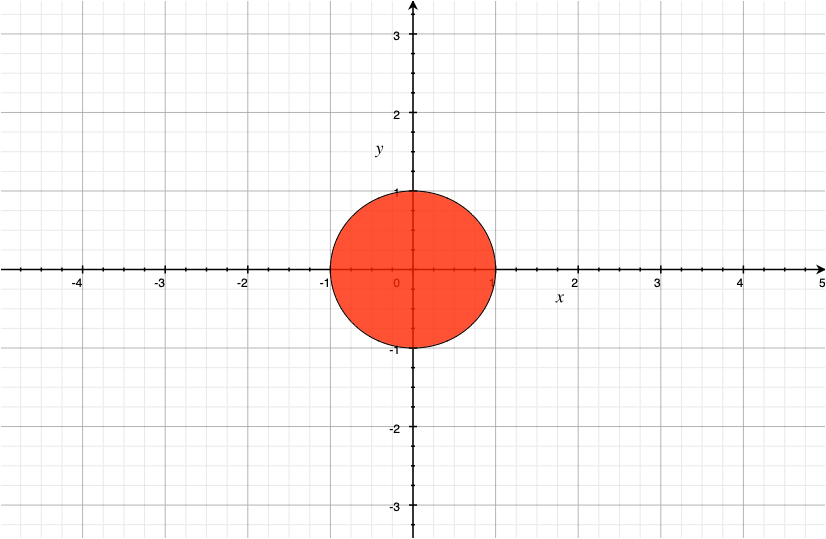
\includegraphics[width=0.7\textwidth]{Analisi2/figures/norma_euclidea.jpg}
    \caption{Grafico di $B(\uline 0, 1)=\{\uline x\in\mathbb R^2\; |\;\sqrt{(x_1-0)^2+(x_2-0)^2}<1\}$.}
    \label{fig:distanza_euclidea_r_1}
\end{figure}

\begin{figure}
    \centering
    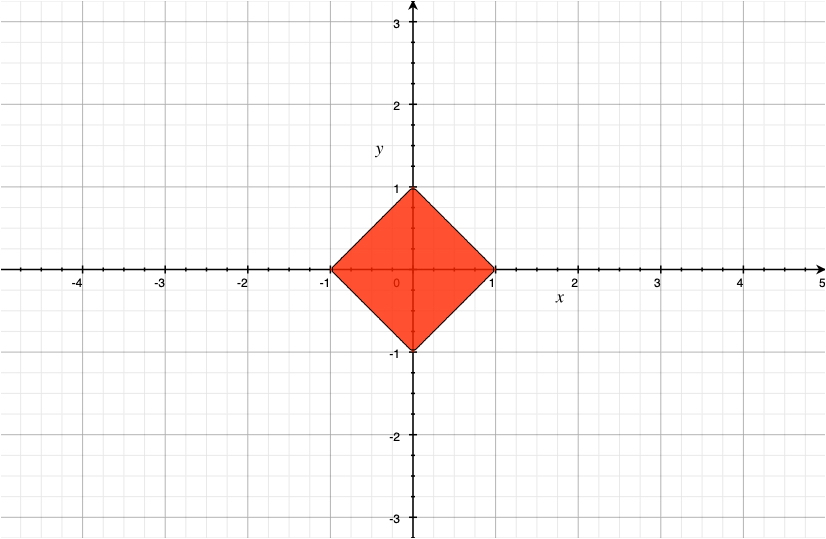
\includegraphics[width=0.7\textwidth]{Analisi2/figures/distanza_tassista.jpg}
    \caption{Grafico di $B(\uline 0, 1)=\{\uline x\in\mathbb R^2\; |\; |x_1-0|+|x_2-0|<1\}$.}
    \label{fig:distanza_tassista_r_1}
\end{figure}

È possibile ora trattare la topologia negli spazi metrici. Le nozioni che saranno date valgono per qualsiasi spazio metrico del tipo $(X,d)$. Per visualizzare i risultati sarà utilizzato $R^n$, con $n=2$ e $d=||\cdot||_2$ (ovvero dove gli intorni sferici sono dischi aperti).

\paragraph{N.B.:} Dato uno spazio metrico $(X,d)$ ed un suo \gls{sottospazio}, allora punto esterno, interno, di frontiera di un sottospazio, spazio aperto e chiuso definiscono la topologia dello spazio.

Vogliamo definire il concetto di limitatezza di un sottospazio metrico. Definendo le Proprietà \ref{prop:successione_convergente_Rn} delle successioni convergenti in $\mathbb R^n$ è stata trattata la limitatezza di una successione continua tramite la distanza. Una successione è un sottoinsieme di $\mathbb R^n$, quindi il concetto può essere generalizzato ad un sottospazio vettoriale $A$ di $X$.

Dati $(X,d)$ e $A\subset X$ (sottospazio di $X$), $x_0\in X,\, r>0$ e $B(\uline x_0, r)=\{x\in X|\, d(x_0,x)<r\}\subset X$, sono date le seguenti definizioni.

\begin{definition} [Sottospazio limitato]\footnote{Slide 7 PDF 8.}
    $A$ è detto limitato se esiste una palla aperta (in $X$) che lo contiene, cioe':
    \begin{equation*}
        \exists r>0,\exists x_0\in X\colon A\subset B(x_0,r).
    \end{equation*}
\end{definition}

Questa definizione riconduce alla limitatezza delle successioni.

\begin{definition}[Punto interno]\footnote{Slide 7 PDF 8.}
    $x_0\in X$ si dice interno ad $A\subset X$ se
    \begin{enumerate}
        \item $x_0\in A$, e
        \item $\exists r>0$ tc $B(x_0, r)\subset A$ \footnote{Ovvero esiste almeno un sottoinsieme sferico di $x_0$ contenuto in $A$.}.
    \end{enumerate}
\end{definition}

\begin{definition}[Punti interni ad $A$]
    I punti interni allo spazio vettoriale $A$ è indicato con $\mathring A$.
\end{definition}

\begin{definition}[Punto esterno]
    $\uline x_0\in X$ si dice punto esterno $A$ se
    \begin{enumerate}
        \item $\uline x_0\notin A$, e
        \item $\exists r>0\; B(\uline x_0, r)\cap A\neq 0$ \footnote{Ovvero: esiste intorno sferico di centro $x_0$ del tutto disgiunto ad $A$.}.
    \end{enumerate}
\end{definition}

\begin{definition}[Punto di frontiera]
    $\uline x_0\in A$ si dice punto di frontiera di $A$ se
    \begin{equation*}
        \exists r>0 \colon B(x_0,r)\cap A \cap A^C \neq 0,
    \end{equation*}
    ovvero se è non è né esterno né interno.
\end{definition}

\paragraph{Notazione punti di frontiera} L'insieme dei punti di frontiera di $A$ è denotato con $\partial A$.

Quindi $x_0$ è un punto di frontiera di $A$ (ovvero $x_0\in\partial A$) se ogni intorno di $x_0$ contiene punti interni ed esterni ad $A$.

\begin{definition}[Insieme aperto]\label{def:insieme_aperto}
    $A$ di dice aperto se $A=\emptyset$, oppure se ogni suo punto è interno ad $A$ (ovvero per ogni punto di $A$ esiste un suo intorno sferico contenuto in $A$).
\end{definition}

\begin{definition}[Insieme chiuso]\footnote{Definizione alternativa libro: $C\subset\mathbb R^n$ si dice chiuso se $A=\mathbb R^n\backslash C$ è aperto.}
    $C$ si dice chiuso se contiene tutti i suoi punti di frontiera, ovvero $\partial C\subset C$.
\end{definition}

\paragraph{N.B.:}\footnote{Slide 2 PDF 9.} Gli insiemi vuoi e $\mathbb R^n$ sono contemporaneamente aperti e chiusi perché entrambi sottoinsiemi di se stessi (inteso come $\emptyset\subseteq\emptyset,\, \mathbb R^n\subseteq\mathbb R^n$). Inoltre, un insieme aperto ha come complementare un insieme chiuso.

\paragraph{N.B.:} Esistono insiemi in $\mathbb R^n$ che non sono né aperti né chiusi.

\begin{definition}[Insieme complementare]\footnote{Definizione non data.}
    Dato $A\subset\mathbb R^n$ insieme aperto, l'insieme complementare di $A$ e'
    \begin{equation*}
        A^C=\{\uline x\in\mathbb R^n\;|\; x\notin A\}.
    \end{equation*}
\end{definition}

\textbf{Considerando lo spazio metrico $(\mathbb R^2, d)$ sono dati esempi in $\mathbb R^2$ di insiemi.}
\begin{example}\footnote{Slide 9 PDF 8.}
    Sia $A_1=\{(x,y)\in\mathbb R^2|x^2+y^2<9\}\subset\mathbb R^2$. $A_1$ è un intorno del cerchio di centro origine e raggio $r=3$. Inoltre $A_1$ è limitato ed aperto e $\partial A_1=\{(x,y)\in\mathbb R^2|x^2+y^2=9\}$. Vedere Figura \ref{fig:A_1_esempio}.
\end{example}

\begin{example}\footnote{Slide 9 PDF 8.}
    Sia $A_2=\{(x, y)\in\mathbb R^2\colon x\neq y^2\}\subset\mathbb R^2$. $A_2$ sono tutti i punti che non sono sulla parabola. $A_2$ non è limitato ed è aperto. $\partial A_2=\{(x,y)\in\mathbb R^2\colon x=y^2\}$. Vedere Figura \ref{fig:A_2_esempio}.
\end{example}

\begin{figure}
    \centering
    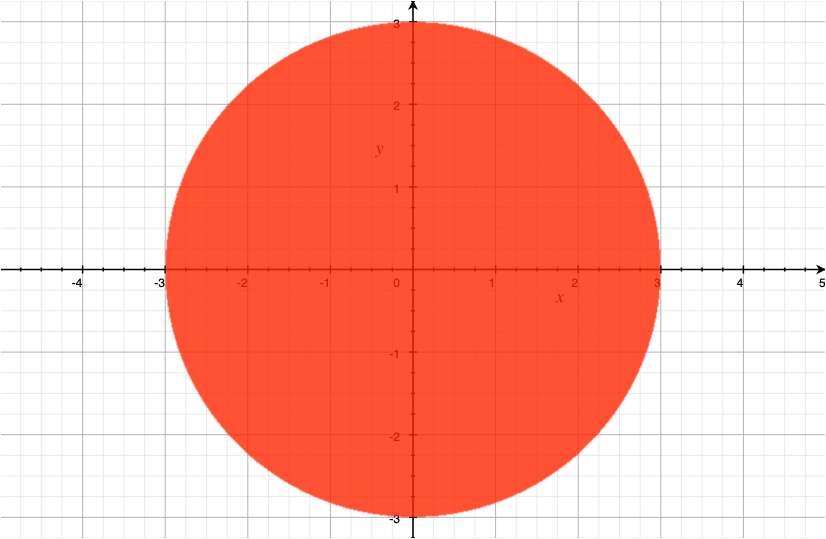
\includegraphics[width=0.7\textwidth]{Analisi2/figures/A1.jpg}
    \caption{Grafico di $A_1=\{(x,y)\in\mathbb R^2|x^2+y^2<9\}$.}
    \label{fig:A_1_esempio}
\end{figure}

\begin{figure}
    \centering
    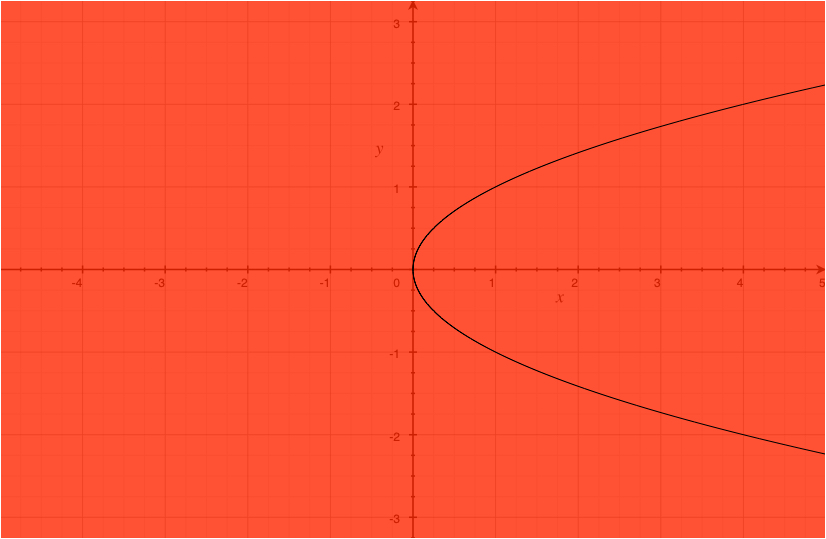
\includegraphics[width=0.7\textwidth]{Analisi2/figures/A2.jpg}
    \caption{Grafico di $A_2=\{(x, y)\in\mathbb R^2\colon x\neq y^2\}$.}
    \label{fig:A_2_esempio}
\end{figure}

\begin{example}\footnote{Slide 10 PDF 8. Questo esempio estende il Teorema \ref{th:esistenza_degli_zeri} degli zeri.}
    Sia $A_3=\{(x,y)\in\mathbb R^2\colon x+y+2\leq 0\}$. L'insieme è formato dai punti che stanno sotto alla funzione $\varphi:y=-x-2$. $A_3$ non è limitato ma chiuso (i punti di frontiera sono la retta). \footnotemark
\end{example}

\footnotetext{Vale il Teorema \ref{th:esistenza_degli_zeri} degli zeri perché gli zeri per la funzione di due variabili. Tale funzione divide in due sottoinsiemi connessi, cioe': il segno delle sottoregioni è costante perché sotto la retta gli elementi hanno segno negativo e sopra positivo. Cosa di dubbia utilità detta dalla prof: Per trovare quale sono i punti in $A_3$ è preso un punto comodo, ad esempio $(-3,0)$ e si sostituisce nella disequazione, determinando così la regione di interesse.}

\begin{definition}[Punto di accumulazione]\footnote{Slide 1 PDF 9.}
    Sia $A\subseteq\mathbb R^n$. $\uline x_0\in\mathbb R^n$ si dice punto di accumulazione per $A$ se \footnote{Comunque mi muovo vicino ad $\uline x_0$ trovo un punto in $A$.}
    \begin{equation*}
        B(\uline x_0, r)\cap (A\backslash\{x_0\})\neq\emptyset.
    \end{equation*}
\end{definition}

\begin{remark}
    Dato $A$ aperto, tutti i punti in $\mathring A$ sono punti di accumulazione.
\end{remark}

\paragraph{N.B.:} I punti di frontiera $\partial A$ possono essere o meno punti di accumulazione di $A$. I punti esterni non sono di accumulazione di $A$.

\begin{definition}[Punto isolato]\footnote{Slide 1 PDF 9.}
    Ogni punto di frontiera in $\partial A$ che non è di accumulazione è detto isolato.
\end{definition}

\paragraph{N.B.:} Non è difficile dimostrare che $\uline x_0$ sia un punto di accumulazione di $A\subseteq\mathbb R^n$ (tramite la definizione stessa di punto di accumulazione). $\uline x_0$ è un punto di accumulazione di $A$ s.se \footnote{Dato l'intorno sferico di centro $\uline x_0$ e raggio qualsiasi si trovano punti in $A$ vicino a $\uline x_0$ nell'intorno sferico. Ovvero: $\uline x_0$ è punto di accumulazione per $A$ s.se diventa quanto scritto dopo la nota.} $\uline x_0$ è il limite di una successione di elementi di $A$ tutti diversi da $x_0$.

\begin{example}\label{ex:norma_in_(1,2)}\footnote{Slide 2 PDF 9.}
    Determinare i punti di accumulazione e quelli di frontiera nel seguente insieme e stabilire se tale insieme è aperto o chiuso.
    \begin{equation*}
        A=\{\uline x\in\mathbb R\;|\; 1<||\uline x||<2\}.
    \end{equation*}
    $\partial A$ è composto dai punti $\uline x$ tc $||\uline x||=1$ e $||\uline x||=2$, ovvero i punti di circonferenza interna ed esterna.\\
    $A$ è un insieme aperto, quindi gli elementi di $\mathring A$ sono punti di accumulazione. Pertanto, $\partial A=\gamma_1\cup\gamma_2$ è l'insieme dei punti di accumulazione.\\
    Vedere Figura \ref{fig:esempio_punti_accumulazione}.
    \begin{figure}
    \centering
    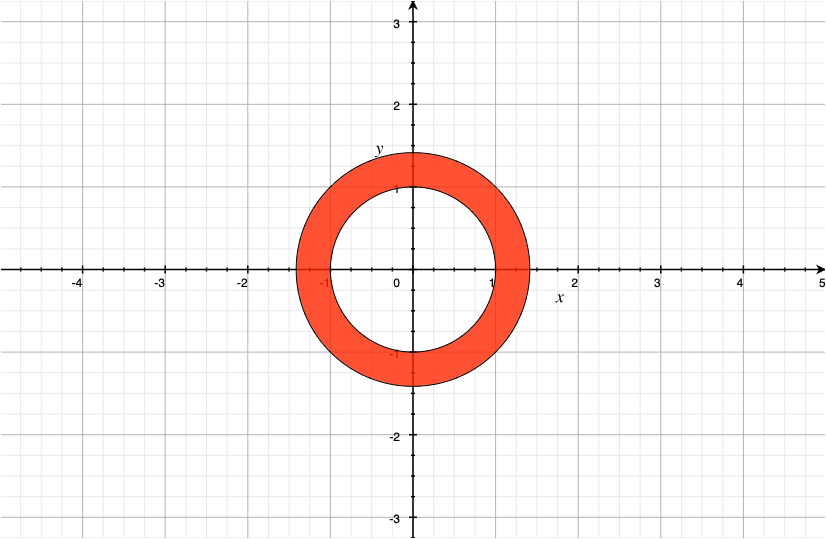
\includegraphics[width=0.5\textwidth]{Analisi2/figures/x2plusy2.jpg}
    \caption{Grafico di $A=\{\uline x\in\mathbb R\;|\; 1<||\uline x||<2\}$.}\label{fig:esempio_punti_accumulazione}
    \end{figure}
\end{example}

\begin{definition}[Chiusura di un insieme]\footnote{Slide 3 PDF 9.}
    La chiusura di $A\subseteq\mathbb R^2$ è denotata da $\bar A\, (\subset\mathbb R^n)$ ed è l'unione di $A$ con i suoi punti di accumulazione.
\end{definition}

\paragraph{N.B.:} $\bar A$ ha le seguenti caratteristiche:
\begin{enumerate}
    \item è un insieme chiuso.
    \item è il più piccolo chiuso che contiene $A$. È possibile dimostrare che $A\in\bar A$ e se $\Bar A=A$ allora $A$ è chiuso.
    \item $\bar A=A\cup\partial A$.
\end{enumerate}

In Analisi 1 una funzione è definita su un dominio (sottoinsieme di $\mathbb R$), ovvero è definita su un intervallo sottoinsiemi di $\mathbb R$. Un intervallo è fatto da un pezzo solo. Anche in Analisi 2 le funzioni sono definite su domini e sono del tipo
\begin{equation*}
    f\colon X\subseteq\mathbb R^n\rightarrow\mathbb R.
\end{equation*}

\begin{definition}[Dominio]\footnote{Slide 3 PDF 9.}
    Un dominio $D$ in $\mathbb R^n$ è la chiusura di un aperto $A\subset\mathbb R^n$, ovvero:
    \begin{equation}\label{eq:dominio_R_n}
        D=A\cup\partial A.
    \end{equation}
\end{definition}

\paragraph{N.B.:} Nell'Esempio \ref{ex:norma_in_(1,2)} il dominio è $D=\{\uline x\in\mathbb R^n\,;\, 1\leq||\uline x||\leq 2$\}, il quale è un insieme chiuso.

\begin{remark}\footnote{Slide 6 PDF 11.}
    Un dominio è un insieme massimale (rispetto all'inclusione su $\mathbb R^n$), ovvero un sottoinsieme di $\mathbb R^n$ massimo nel quale la funzione è ben definita.
\end{remark}

\begin{example}
    Una sfera chiusa contenuta in $\mathbb R^n$ è un dominio. Una sfera chiusa unito ad un punto isolato (esterno) non è un domino.
\end{example}

\subsection{Limite e continuità}
È stato trattato quanto precede sui punti di accumulazione per introdurre il concetto di limite in $\mathbb R^n$, quindi per funzioni di più variabili, con valori in $\mathbb R$. Inoltre, tramite il concetto di limite è possibile introdurre il concetto di continuità di una funzione.

\begin{definition}[Limite di funzione]\label{def:limite_funzione_piu_variabili}\footnote{Slide 4 PDF 9.}
    Data
    \begin{equation*}
        \begin{aligned}
            f\colon A\subseteq\mathbb R^n & \rightarrow \mathbb R\\
            \uline x &\mapsto f(\uline x)
        \end{aligned}
    \end{equation*}
    e sia $\uline x_0=(x_0^1,\hdots,x_0^n)\in\mathbb R^n$ un punto di accumulazione per $A$. Si dice che $f$ tende a $\ell\in$\gls{Rext}$=\mathbb R\cup\{\pm\infty\}$ per $\uline x$ che tende a $\uline x_0$ e si scrive
    \begin{equation}\label{eq:limite_funzione_piu_variabili}
        \lim_{\uline x\rightarrow\uline x_0}f(\uline x)=\ell \quad\text{ovvero}\quad f(\uline x)\overset{\footnotemark}{\underset{\uline x\rightarrow\uline x_0}{\longrightarrow}}\ell
    \end{equation}
    \footnotemark se per ogni intorno $U\subset\overline{\mathbb R}$ di $\ell$ esiste un intorno sferico di $\uline x_0$, ovvero:
    \begin{equation*}
        \exists r>0,\, I(\uline x_0, r)=B(\uline x_0,r)\subset\mathbb R^2 \text{ tc } f(\uline x)\in U\quad \forall\uline x\in I(\uline x_0,r)\cap(A\backslash\{\uline x_0\}).
    \end{equation*}
\end{definition}

\addtocounter{footnote}{-1}
\footnotetext{$f(\uline x)\underset{\uline x\rightarrow\uline x_0}{\longrightarrow}\ell$ significa che $f(\uline x)$ appartiene all'intorno di $\ell$ non appena $\uline x$ è nell'intorno sferico di $\uline x_0$. Stessa definizione di Analisi 1.}

\stepcounter{footnote}
\footnotetext{Dato che $\ell\in\overline{\mathbb R}$, è possibile parlare di intorni di infinito, ovvero semirette finite del tipo $(n,+\infty)$ o $(-\infty, n)$.}

\paragraph{N.B.:} Il limite di funzione appena definito è una operazione definita su $\overline{\mathbb R}$ e quindi $\ell$ può essere un numero reale o $\pm\infty$.\\
La Definizione \ref{def:limite_funzione_piu_variabili} di limite di funzione è la stessa definizione di limite di Analisi 1, si distingue per $\pm\infty$. Quando $\ell=\pm\infty$ significa che esiste $M$ tale che $f$ da un certo punto in poi è maggiore di $M$, quindi $f$ ha valori appartenenti alla semiretta $(M,+\infty)$ (intorno di $+\infty$). Per avere una notazione compatta è utilizzato un certo intorno, come sopra.

La Definizione \ref{def:limite_funzione_piu_variabili} di limite di funzione è equivalente alle Definizioni \ref{def:limite_epsilon_delta_convergente_piu_variabili} e \ref{def:limite_epsilon_delta_divergente_piu_variabili} di limite convergente e divergente $\varepsilon$-$\delta$ seguenti.

\begin{definition}[Limite finito $\varepsilon$-$\delta$]\label{def:limite_epsilon_delta_convergente_piu_variabili}\footnote{Slide 4 PDF 9.}
    \begin{equation*}
        \lim_{\uline x\rightarrow\uline x_0}f(\uline x)=\ell\in\mathbb R
    \end{equation*}
    è finito se
    \begin{equation}
        \forall\varepsilon>0\;\exists\delta>0\quad\text{tc}\quad \underbrace{\overbrace{|f(\uline x)-\ell|}^{d(f(\uline x,\ell))\in\mathbb R}<\varepsilon}_{\footnotemark}\quad \underbrace{\forall\uline x\in(A\backslash\{\uline x_0\}) \text{ con } ||\uline x-\uline x_0||<\delta \text{ e } \uline x\in B(\uline x_0,\delta)}_{\footnotemark}.
    \end{equation}
\end{definition}

\addtocounter{footnote}{-1}
\footnotetext{Equivale a $\underbrace{\ell-\varepsilon<f(\uline x)<\ell +\varepsilon\equiv B(\ell, \varepsilon)}_{\subset\mathbb R}\ni f(\uline x)$.}

\stepcounter{footnote}
\footnotetext{Può essere espresso come segue: $\forall\uline x\in A$ con $0<||\uline x - \uline x_0||<\delta$. La norma deve essere maggiore stretta di 0 perché è necessario che $\uline x\neq \uline x_0$.}

In modo analogo sono definiti i limiti divergenti.
\begin{definition}[Limite divergente $\varepsilon$-$\delta$]\label{def:limite_epsilon_delta_divergente_piu_variabili}\footnote{Libro PG 42.}
    \begin{equation*}
        \lim_{\uline x\rightarrow\uline x_0}f(\uline x)=\pm\infty
    \end{equation*}
    è divergente a $\pm\infty$ se
    \begin{equation}\label{eq:limite_epsilon_delta_divergente_piu_variabili}
        \forall M>0\;\exists\delta>0\quad\text{tc}\quad f(\uline x)>M \quad \forall\uline x\in(A\backslash\{\uline x_0\}) \text{ con } ||\uline x-\uline x_0||<\delta \text{ e } \uline x\in B(\uline x_0,\delta).
    \end{equation}
\end{definition}

Il limite di una funzione segue la stessa algebra e le stesse regole che in Analisi 1.
\begin{property}[Proprietà limite di funzione]\footnote{Slide 5 PDF 9.}
    Il limite di funzione definito come (\ref{eq:limite_funzione_piu_variabili}) ha le seguenti proprietà:
    \begin{enumerate}
        \item se esiste è unico,
        \item il limite di somma e prodotto di funzioni (reali in più variabili) sono uguali alla somma e prodotto di limiti (se esistono),
        \item il limite del rapporto (di quoziente) è uguale al rapporto (quoziente) fra i limiti (se ben definiti, ovvero denominatore diverso da 0 e definita l'operazione di quoziente).
        \item $\lim_{\uline x\rightarrow\uline x_0}c\cdot f(\uline x)=c\cdot\lim_{\uline x\rightarrow \uline x_0}f(\uline x)$
    \end{enumerate}
\end{property}

\paragraph{N.B.:} Somma (la sottrazione è come somma cambiata di segno: $x-y=x+(-1) y$) e prodotto di funzione sono intese come algebriche.

\paragraph{Suggerimento:} prima di calcolare un limite verificare se esiste.

\begin{example}\footnote{Slide 5 PDF 9.}
    Sia
    \begin{equation*}
        f(x,y)=\frac{x^2}{\sqrt{x^2+y^2}}\colon A=\mathbb R^2\backslash\{(0,0)\}\rightarrow\mathbb R.
    \end{equation*}
    $\uline 0\notin A$ è un punto di accumulazione per $A$.
    \footnote{Vogliamo mostrare, tramite la definizione di limite, cosa accade vicino l'origine della funzione.} Mostriamo che
    \begin{equation*}
        \lim_{(x,y)\rightarrow(0,0)}f(x,y)=0.\footnotemark
    \end{equation*}
    \footnotetext{Quindi è necessario dimostrare che comunque preso un intorno in $\mathbb R^2$ di $\uline 0$ esiste un intorno di raggio $\delta$ nell'origine di punti di $A$ diversi da $(0,0)$ per cui $f$ è nell'intorno di $\uline 0$ non appena le coppie $(x,y)\in I_\delta((0,0))$.}
    È necessario dimostrare quindi che
    \begin{equation*}
        \lim_{(x,y)\rightarrow(0,0)}\frac{x^2}{\sqrt{x^2+y^2}}=0
    \end{equation*}
    ovvero (tramite (\ref{eq:limite_epsilon_delta_divergente_piu_variabili}))
    \begin{equation*}
        \forall\varepsilon>0\,\exists\delta=\delta_\varepsilon>0,\, \underbrace{|f(x,y)-0|<\varepsilon}_{d(f(x,y),\uline 0)\in\mathbb R}\quad \forall(x,y)\in A \text{ con } \underbrace{0<\sqrt{x^2+y^2}<\delta}_{\footnotemark}.
    \end{equation*}
    \footnotetext{$B(\uline 0, \delta)=\{\uline x\in\mathbb R^2\,|\, d(\uline x,\uline 0)=||\uline x-\uline 0||<\delta\}$.}
    \footnote{È necessario verificare che $0<\sqrt{x^2+y^2}<\delta$.} È possibile osservare che
    \begin{equation*}
        0\leq\underbrace{\frac{x^2}{\sqrt{x^2+y^2}}\leq\frac{x^2+y^2}{\sqrt{x^2+y^2}}=\sqrt{x^2+y^2}}_{\footnotemark},
    \end{equation*}
    dimostrando che
    \begin{equation}\label{eq:esempio_limite}
        0\leq f(x,y)\leq \sqrt{x^2+y^2}=\delta=\delta_\varepsilon\quad \forall(x,y)\in A
    \end{equation}
    e dunque
    \begin{equation*}
        \forall\varepsilon>0\;\exists\delta = \sqrt{x^2+y^2}\quad \text{ tc }\quad 0\leq f(x,y)\leq\varepsilon\quad\forall(x,y)\neq(0,0)\quad\text{ tc }\quad \sqrt{x^2+y^2}=\delta_\varepsilon<\varepsilon.
    \end{equation*}
    Quindi, da (\ref{eq:esempio_limite}), $|f(x,y)-0|<\varepsilon$.
\end{example}
\footnotetext{Applicata maggiorazione con un'espressione con valore \gls{infinitesimo}, ovvero $\sqrt{x^2+y^2}$. $\sqrt{x^2+y^2}$ è un infinitesimo ed è uguale a $\delta$ (della Definizione \ref{def:limite_epsilon_delta_convergente_piu_variabili} di limite finito $\varepsilon$-$\delta$).}

Il problema principale dei limiti è dimostrare l'esistenza. Le funzioni in più variabili tendono a non avere limite. Ci sono teoremi per dimostrare che il limite di una funzione in più variabili non esiste. Inoltre, per le funzioni in più variabili, può essere utile trasformare le coordinate cartesiane in coordinate polari per semplificare il calcolo dei limiti.

\begin{example}\footnote{Slide 7 PDF 9.}
    Mostrare che 
    \begin{equation*}
        \lim_{(x,y)\rightarrow(0,0)}\frac{x}{\sqrt{x^2+y^2}}
    \end{equation*}
    non esiste. $f=\frac{x}{\sqrt{x^2+y^2}}\colon A=\mathbb R^2\backslash\{\uline 0\}\rightarrow\mathbb R$.\\
    \footnotemark È necessario mostrare cosa accade in un intorno di centro $(0,0)$ e raggio $r=\delta$. È possibile muoversi vicino a $(0,0)$ sull'asse $y$ (quindi con $x=0$). Dunque è considerata $f(0,y)=0$ al variare di $y$ (quindi il candidato dovrebbe essere 0).\\
    Muovendosi sull'asse $x$, con $y=0$, la funzione assume i seguenti valori:
    \begin{equation}\label{eq:esempio_limiti_1}
        f(x,0)=\frac{x}{\sqrt{x^2}}=\frac{x}{|x|}=
        \begin{cases}
            1, & x>0,\\
            -1,& x>0.
        \end{cases}
    \end{equation}
    Quindi il limite non è unico: il valore del limite dipende dalla direzione con la quale $\uline x$ si avvicina a $(0,0)$. Ovvero $\nexists\lim_{(x,y)\rightarrow(0,0)}f(x,y)$.

    \begin{figure}
    \centering
    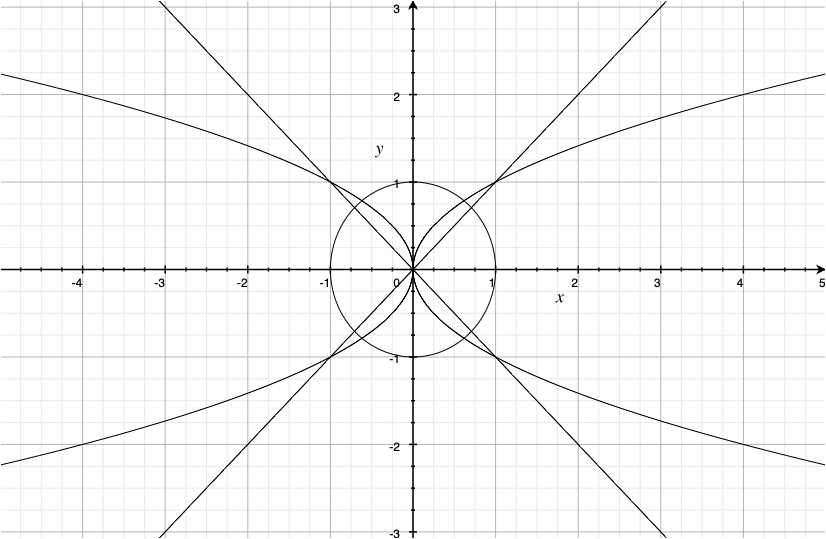
\includegraphics[width=0.5\textwidth]{Analisi2/figures/cammini_0,0.jpg}
    \caption{Grafico di alcuni possibili cammini che "portano" all'origine $(0,0)$.}\label{fig:cammini_0,0}
    \end{figure}
\end{example}

\footnotetext{$f$ è definita su tutto $\mathbb R^2$ tranne nell'origine. Vogliamo vedere cosa accade ad $f$ nell'origine tramite la definizione di limite. Muoversi in $\mathbb R$ (ovvero sul piano) nell'\gls{asse reale} vicino ad $x_0$ significa stare a sinistra o a destra di $x_0$ ma entro $\delta$. In $\mathbb R^2$ le direzioni sono infinite, quindi è possibile muoversi vicino ad $x_0$ in tutte le direzioni. Per semplicità è scelto un cammino semplice. Con cammino semplice si intende percorrere le assi $x,y$, le bisettrici, parabole, come in Figura \ref{fig:cammini_0,0}, o un qualsiasi altro degli infiniti cammini che portano all'origine. Quindi in $\mathbb R^2$ è più complesso che in Analisi 1 calcolare il limite di una funzione.}

\paragraph{Deduzioni dall'esempio:} L'esistenza del limite non può dipendere da come ci si avvicina al punto "problematico", ovvero il limite deve essere lo stesso indipendentemente dalla direzione di avvicinamento di $(x,y)$ al punto $(x_0, y_0)$ e non dipendere dal modo (ovvero dalla direzione di avvicinamento). Una direzione nel piano è un vettore modulo, ovvero $\uline x\in\mathbb R$ tale che $||\uline v||=1$ (in genere ad ogni vettore è associata una direzione sul piano).  In generale si parla di direzione quando un vettore è normalizzato, ovvero quando $||\uline x||=1$. Quindi, quando il limite esiste ed è unico significa che il limite non deve dipendere dalla direzione e/o dal cammino scelto con il quale il punto $P=(x,y)$ si avvicina al punto $P_0=(x_0,y_0)$.  Il cammino può essere inteso come una bisettrice, parabola, o qualsiasi alta curva come in Figura \ref{fig:cammini_0,0}. In altre parole ancora: trovati due cammini percorrendo il quali $P$ si avvicina a $P_0$, è possibile provare che se tendono a $P_0$ e danno limiti diversi allora il limite non esiste.

\paragraph{N.B.:} Potrebbe capitare che due cammini portino a due valori reali distinti (già questo permette di determinare che il limite non esiste).

\paragraph{N.B.:} Il punto "generico" di un limite di funzione in più variabili $\uline x=(x_0,x_1,\hdots, x_n)\in\mathbb R^n$ può essere denotato con $P$ ed il punto di accumulazione $\uline x_0=(x_0^1,x_0^2,\hdots, x_0^n)\in\mathbb R^n$ come $P_0$. Inoltre, data $f:A\subset\mathbb R^2\rightarrow\mathbb R$ con $(x_0,y_0)$ punto di accumulazione per $A$, per descrivere l'operazione di limite di funzione può essere utilizzata la notazione $P,\, P_0$ così risaltare il carattere geometrico della funzione (ad ogni coppia è associata un punto sul piano e viceversa per la corrispondenza biunivoca del piano cartesiano tra coppie ordinata e punti sul piano). Ovvero, dati $P=(x,y), P_0=(x_0,y_0)$,
\begin{equation*}
    \lim_{(x,y)\rightarrow(x_0,y_0)}f(x,y)=l\in\mathbb R \quad\text{equivale a}\quad \lim_{P\rightarrow P_0}f(P)=P_0.
\end{equation*}

La seguente proposizione permette di affermare quando un limite esiste (formalizzando quanto scritto sopra).

\begin{proposition}[Condizione necessaria per l'esistenza del limite]\footnote{Slide 8 PDF 9.}
    Sia $f\colon A\subset\mathbb R^2\rightarrow\mathbb R$ e $(x_0, y_0)$ punto di accumulazione per $A$. Se
    \begin{equation*}
        \lim_{(x,y)\rightarrow(x_0,y_0)} f(x,y)=\ell
    \end{equation*}
    allora $\forall C\subset A$ deve valere
    \begin{equation*}
        \lim_{C\ni(x,y)\rightarrow (x_0,y_0)}f(x, y)=\ell.
    \end{equation*}
\end{proposition}

\paragraph{N.B.:} trovare $n$ cammini che confermano che il limite è valido non significa che il limite esista. La Proposizione è una condizione necessaria ma non sufficiente.

\begin{remark}
    è possibile osservare che come condizione necessaria per l'esistenza del limite è spesso utilizzato il fatto che esistano, e che siano uguali fra loro, i limiti lungo le rette parallele agli assi coordinati di equazione $y=y_0\in\mathbb R$ e $x=x_0\in\mathbb R$ (costanti), ottenendo come condizione necessaria per l'esistenza
    \begin{equation*}
        \lim_{x\rightarrow x_0}f(x,y_0)=\ell=\lim_{y\rightarrow y_0}f(x_0, y).
    \end{equation*}
\end{remark}

\begin{exercise}[Per casa]\label{exercise:limite_non_esiste_casa}
    Mostrare che il seguente limite non esiste
    \begin{equation*}
        \lim_{(x,y)\rightarrow(0,0)}\frac{xy}{x^2+y^2}.
    \end{equation*}
    Consigli su come farlo: Prima provare cosa accade sugli assi coordinati. Seconda cosa provare qualche curva.\\
    \textbf{Svolgimento:}
    \begin{equation*}
        \lim_{\underset{x=y}{(x,y)\rightarrow(0,0)}}f(x,y)=\lim_{y\rightarrow 0}f(y,y)=\lim_{y\rightarrow 0}\frac{y\cdot y}{y^2+y^2}=\lim_{y\rightarrow 0}\frac{\cancel{y^2}}{2\cancel{y^2}}=\frac{1}{2}=\lim_{x\rightarrow 0}\frac{x\cdot x}{x^2+x^2}=\lim_{x\rightarrow 0}f(x,x)=\lim_{\underset{y=x}{(x,y)\rightarrow(0,0)}}f(x,y).
    \end{equation*}
    \begin{equation*}
       \lim_{\underset{y=x^2}{(x,y)\rightarrow(0,0)}}f(x,y)=\lim_{x\rightarrow 0}\frac{x\cdot x^2}{x^2+(x^2)^2}=\lim_{x\rightarrow 0}\frac{x^{\cancel{3}}}{\cancel{x^2}(1+x^2)}=0.
    \end{equation*}
    Dato che $0\neq \frac{1}{2}$, il limite non esiste.
\end{exercise}

\begin{definition}[Continuità di funzione]\footnote{Slide 1 PDF 10.}\label{def:continuita_funzione_n_variabili}
    Sia $f\colon A\subseteq\mathbb R^n\rightarrow\mathbb R$ e (supposto $n=2$) sia $P_0=(x_0,y_0)\in A$. Se $P_0$ è punto di accumulazione per $A$, $f$ si dice continua in $P_0$ se
    \begin{equation}\label{eq:limite_continuita}
        \lim_{(x,y)\rightarrow(x_0,y_0)}f(x,y)=f(x_0,y_0)\quad \left(\text{per } n>2\; \lim_{\uline x\rightarrow\uline x_0}f(\uline x)=f(\uline x_0)\right).
    \end{equation}
    Se $P_0$ è un punto isolato per $A$ per convenzione si pone $f$ continua in tale punto.
\end{definition}

\begin{definition}[Funzione continua]\footnote{Slide 1 PDF 10.}
    Sia $f\colon A\subset\mathbb R^n\rightarrow\mathbb R$. $f$ si dice continua in $A$ se è continua in ogni punto di $A$.
\end{definition}

Per mostrare la continuità di una funzione in un punto è necessario quini mostrare quanto appena scritto.

\begin{example}\footnote{Slide 1 PDF 10.}
    Siano $f(x,y)=x$ e $g(x,y)=y$, quindi $f,g\colon A=\mathbb R^2\rightarrow\mathbb R$ (ovvero $f$ e $g$ sono funzioni continue in $A=\mathbb R^2$).\\
    Mostriamo che $f(x,y)$ è continua in $\forall P_0=(x_0,y_0)\in\mathbb R^2$. È necessario mostrare che
    \begin{equation*}
        \lim_{(x,y)\rightarrow(x_0,y_0)}f(x,y)=f(x_0,y_0)\in\mathbb R\; \text{(reale finito)}.
    \end{equation*}
    \footnote{È necessario che il limite di $f$ esiste ed è finito utilizzando la Definizione \ref{def:limite_epsilon_delta_convergente_piu_variabili} di limite finito.} Quindi è necessario mostrare che
    \begin{equation*}
        \forall\varepsilon>0\;\exists\delta=\delta(\varepsilon)>0 \text{ tc } |f(x,y)-f(x_0,y_0)|<\varepsilon \text{ se } (x,y)\in\mathbb R^2\cap B((x_0,y_0),\delta)\; \forall (x,y)\in\mathbb R^2, \underbrace{\sqrt{(x-x_0)^2+(y-y_0)^2}}_{d(P,P_0)}<\delta.
    \end{equation*}
    (Quindi è necessario mostrare che) $\sqrt{(x-x_0)^2+(y-y_0)^2}<\delta\iff|\equalto{x}{f(x,y)}-x_0|<\varepsilon$.\\
    (È possibile scrivere in modo diverso $|\cdot|$)  $0\leq|x-x_0|\overset{\footnotemark}{=}\sqrt{(x-x_0)^2}\leq\sqrt{(x-x_0)^2+(y-y_0)^2}<\delta$, quindi la definizione vale in $\delta=\varepsilon$.\\
    (Analogo procedimento con $g(x,y)=y^2$.)
\end{example}
\footnotetext{Trasformazione in radice aritmetica di un numero non negativo.}

\paragraph{N.B.:} Per le funzioni in una variabile ci sono opportuni teoremi sulle operazioni algebriche e sulla continuità. Per le funzioni in più variabili valgono gli stessi risultati con opportune considerazioni. Pertanto, è necessario estendere tali teoremi su domini in $\mathbb R^n$. Concetti che non coincidono con fra funzioni in una variabile ed in più variabili sono differenziabilità e derivabilità:
\begin{itemize}
    \item Per le funzioni in una variabile coincidono,
    \item Per le funzioni in più variabili il concetto di derivabilità è generalizzato nel concetto di differenziabilità. La differenziabilità è una proprietà più forte della derivabilità. La derivabilità in $\mathbb R^n$ non ha le stesse proprietà che in $\mathbb R$.
\end{itemize}

Il prossimo Teorema riguarda l'algebra delle funzioni in più variabili.
\begin{theorem}\label{th:algebra_funzioni_piu_variabili}\footnote{Slide 2 PDF 10.}
    Siano $f$ e $g$ funzioni di più variabili a valori reali continue (negli opportuni domini o in un punto), allora
    \begin{enumerate}
        \item $f\pm g$ (somma algebrica) e $f\cdot g$ sono continue (negli opportuni domini),
        \item (quoziente) se $g\neq 0$ allora $\frac{f}{g}$ è continua,
        \item (Legge di esponenziazione) se $g>0$ allora $f^g$ è continua,
        \item la funzione composta $g\circ f$ è continua dove è definita.
    \end{enumerate}
\end{theorem}

\begin{remark}\footnote{Slide 3 PDF 10.}
    Sia $f\colon A\subseteq\mathbb R^n\rightarrow\mathbb R$ e $g:J\subseteq\mathbb R\rightarrow\mathbb R$, allora $g\circ f\colon \mathbb\rightarrow\mathbb R$ segue il seguente processo
    \begin{equation*}
        \uline x\mapsto \underset{\underset{\mathbb R,\, D(g)}{\vertin}}{f(\uline x)}\mapsto g(f(\uline x)).
    \end{equation*}
    Per poter valutare $g\circ f$, $f(x)$ deve appartenere al dominio di $g$, ovvero $Imm(f)=f(A)\subseteq D(g)\subseteq\mathbb R$.
\end{remark}

\paragraph{N.B.:} Utilizzando il precedente Teorema \ref{th:algebra_funzioni_piu_variabili} è possibile affermare che le seguenti funzioni elementari sono continue:
\begin{itemize}
    \item Polinomi in più variabili,
    \item Funzioni razionali (quoziente di polinomi), dove il denominatore è diverso da 0 (ovvero le funzioni sono ben definite),
    \item Esponenziali in più variabili (esempio: $e^{x^2+y^2}$)
    \item Funzioni trigonometriche e loro inverse.
\end{itemize}
Inoltre è possibile affermare che tutte le funzioni elementari combinate con somme algebriche, prodotti ed esponenziazioni sono continue.

\begin{example}
    Data la funzione (razionale in due variabili)
    \begin{equation*}
        f(x,y)=\frac{e^{\frac{x^2-y^3}{x^2+y^2}}}{\cos(y-x)},
    \end{equation*}
    determinare il suo insieme di definizione $A\subseteq\mathbb R^2$, disegnarlo e stabilire la metrica topologica.
    \begin{itemize}
        \item (Dominio)
        \begin{equation*}
            \begin{matrix}
                \boldsymbol A&=&\{(x,y)\in\mathbb R^2;x^2+y^2\neq 0,\; \cos(y-x)\neq 0\}\\
                &=&\{(x,y)\in\mathbb R^2;(x,y)\neq(0,0),\, y-x\neq \frac{\pi}{2}+k\pi,\, \forall k\in\mathbb Z\}\\
                &=&\boldsymbol{\{(x,y)\in\mathbb R^2;(x,y)\neq(0,0),\, y\neq x + \frac{\pi}{2}+k\pi,\, \forall k\in\mathbb Z\}}.
            \end{matrix}
        \end{equation*}
        \item (Disegno) Vedere Figura \ref{fig:esempio_dominio_analisi2}. [Il dominio è la parte in blu che non comprende le rette $y=x+\frac{\pi}{2}+k\pi$.]
        \item (Metrica topologica) Il dominio $A$ è l'unione di aperti e non è limitato.
    \end{itemize}
    \begin{figure}
    \centering
    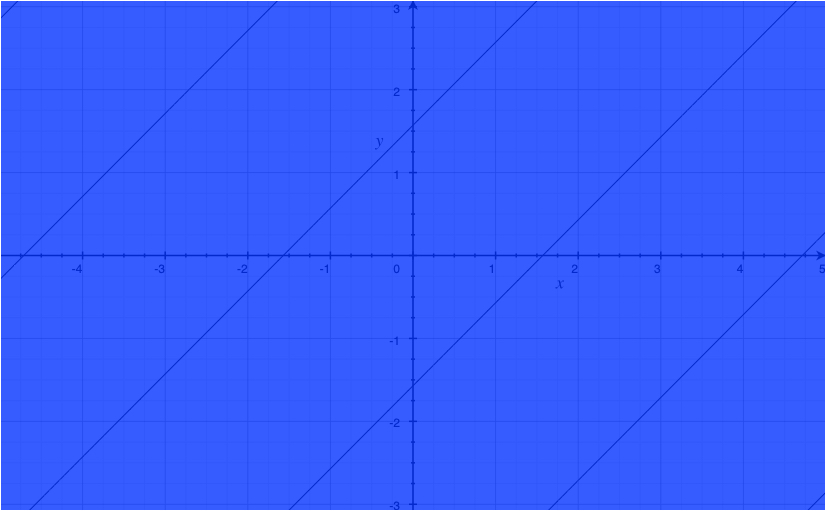
\includegraphics[width=0.5\textwidth]{Analisi2/figures/A_dom.jpg}
    \caption{Grafico di $A=\{(x,y)\in\mathbb R^2;(x,y)\neq(0,0),\, y\neq x + \frac{\pi}{2}+k\pi,\, \forall k\in\mathbb Z\}$.}\label{fig:esempio_dominio_analisi2}
    \end{figure}
\end{example}

\begin{example}\footnote{Slide 5 PDF 10.}
    Data la funzione
    \begin{equation*}
        f(x,y)=
        \begin{cases}
            \frac{e^{(x-1)+(y-1)}-1}{\sqrt{(x-1)^2+(y-1)^2}} &\text{se } (x,y)\neq (1,1),\\
            0 &\text{se } (x,y)=(1,1),
        \end{cases}
    \end{equation*}
    studiarne la continuità sul suo dominio di definizione.\\
    $f$ è definito su $\mathbb R^2$, ovvero: $f\colon\mathbb R^2\rightarrow\mathbb R$.\\
    \footnote{Studiare il problema significa studiare la continuità. Per le conseguenze del Teorema \ref{th:algebra_funzioni_piu_variabili}, $f$ è continua in ogni punto di $\mathbb R^2$ diverso da $(1,1)$ perché funzione quoziente. Per verificare la continuità è necessario che il limite di $f(x,y)$ per $(x,y)\rightarrow (1,1)$ converga a 0, ovvero quanto segue alla nota.} Affinché $f$ risulti continua in tutto $\mathbb R^2$ allora (deve esistere il limite e valere 0, ovvero)
    \begin{equation*}
        \lim_{(x,y)\rightarrow(1,1)} f(x,y)=\lim_{(x,y)\rightarrow(1,1)}\frac{e^{(x-1)+(y-1)}-1}{\sqrt{(x-1)^2+(y-1)^2}}=f(1,1)=0.
    \end{equation*}
    Studiamo dunque $\lim_{(x,y)\rightarrow(1,1)}f(x,y)$. \footnote{Ciò che è richiesto è di provare prima che il limite esista, che sia finito e che coincida con valore della funzione nel punto. In questo caso non può essere $\pm\infty$. Se il limite esiste ed ha un valore diverso da 0 nel punto $(1,1)$ ed è necessario rendere la funzione continua nel punto, allora è possibile ridefinire la funzione in quel punto con il valore del limite, come per Analisi 1.}\footnote{Il limite fa capire cosa accade vicino al punto $(1,1)$. È possibile decidere di muoversi lungo qualsiasi cammino per avvicinarsi al punto. Quindi è possibile muovesi lungo la retta verticale seguendo i punti $(x,y)\in\{1\}\times\mathbb R\backslash\{1\}$ (come in Figura \ref{fig:esempio_f_1_y}, ovvero ciò che segue alla nota.)} Muovendosi lungo i $x=1$ con $y\neq 1$ è considerata
    \begin{equation*}
        f(1, y)=\frac{e^{y-1}-1}{\sqrt{(y-1)^2}}.
    \end{equation*}
    Quindi (con $y$ che tende ad 1 lungo la retta in Figura \ref{fig:esempio_f_1_y} dall'alto o dal basso)
    \begin{equation*}
        \lim_{\underset{x=1}{(x,y)\rightarrow(1,1)}}f(x,y)=\lim_{y\rightarrow 1}f(1,y)=\lim_{y\rightarrow 1}\frac{e^{y-1}-1}{\sqrt{(y-1)^2}}=\lim_{y\rightarrow 1}\frac{e^{y-1}-1}{(y-1)}\overset{\footnotemark}{=}
        \begin{cases}
            1 &\text{se } y>1\\
            -1 &\text{se } y<1
        \end{cases}
    \end{equation*}
    \footnotetext{Utilizzato il limite notevole $\lim_{t\rightarrow 0}\frac{e^t-1}{t}=1$. Tale limite è dovuto allo sviluppo di Taylor: $\lim_{t\rightarrow 0} e^t=1+t+o(t)$.}
    Quindi il limite non esiste e la funzione non è continua nel punto $(1,1)$. Ovvero: non vale la definizione di continuità.
    \begin{figure}
    \centering
    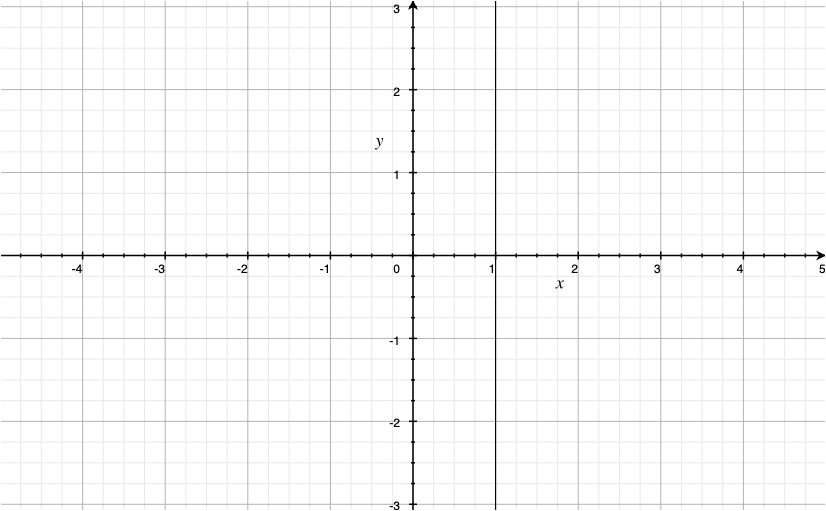
\includegraphics[width=0.5\textwidth]{Analisi2/figures/esempio_f_1_y.jpg}
    \caption{Grafico del cammino utilizzato per avvicinarsi al punto $(1,1)$.}\label{fig:esempio_f_1_y}
    \end{figure}
\end{example}

\paragraph{N.B.:} La definizione di continuità di una funzione stabilisce che la funzione $f(x,y)$, definita come $f\colon A\subset\mathbb R^2\rightarrow\mathbb R$, è continua in $(x_0, y_0)\in A$ se $\lim_{(x, y)\rightarrow (x_0,y_0)}f(x,y)=f(x_0, y_0)$. Questo non vale se il limite non esiste. La continuità vale se il limite esiste, è finito e coincide con il valore della funzione nel punto $(x_0, y_0)$. Può capitare che il limite non esista, sia infinito, oppure che esista finite ma con valore diverso da quello della funzione nel punto $(x_0, y_0)$. Quindi, per studiare la continuità è necessario studiare cosa accade nell'intorno del punto $(x_0, y_0)$.

\paragraph{N.B.:} Ogni esercizio che ha a che fare con i limiti può essere svolto nuovamente utilizzando le coordinate polari.

\begin{example}\footnote{Slide 7 PDF 10.}
    Calcolare l'esistenza del seguente limite:
    \begin{equation*}
        \lim_{(x,y)\rightarrow(0,0)}\frac{\sin^2(x)-\cos(y^2)}{x^2+y^2}.
    \end{equation*}
    Lungo l'asse $x$: ($y=0$ con $x\neq 0$)
    \begin{equation*}
        \lim_{\underset{y=0}{(x,y)\rightarrow(0,0)}}\frac{\sin^2(x)-\cos(y^2)}{x^2+y^2}=\lim_{x\rightarrow 0}\frac{\sin x^2}{x^2}=1.
    \end{equation*}
    Lungo l'asse $y$: ($y=0$ con $x\neq 0$)
    \begin{equation*}
        \lim_{y\rightarrow 0}\frac{-\sin y^2}{y^2}=-1
    \end{equation*}
    $-1\neq 1$, quindi non esiste limite unico.\\
    Nell'esempio sono stati trovati due cammini che danno luogo a limiti diversi. La condizione necessaria è che se la funzione ha limite $\ell$ allora per ogni cammino percorso per avvicinarsi al punto (qualsiasi sia la direzione) allora il limite deve valere $\ell$.
\end{example}

\begin{example}\footnote{Slide 8 PDF 10.}
    Verificare l'esistenza del seguente limite.
    \begin{equation*}
        \lim_{(x,y)\rightarrow(0,0)}\frac{\arctan(x+y)^2}{x^2}.
    \end{equation*}
    Lungo l'asse $x$: ($y=0$ con $x\neq 0$)
    \begin{equation*}
        \lim_{\underset{y=0}{(x,y)\rightarrow(0,0)}}f(x, y)= \lim_{x\rightarrow 0}\frac{\arctan(x^2)}{x^2}\overset{\footnotemark}{=}1.
    \end{equation*}
    \footnotetext{Utilizzato il limite notevole. Tramite la formula di Taylor: $\arctan t=0+\left.\frac{1}{1+t^2}\right|_{t=0}\cdot t +o(t)=t+o(t)$.}
    Lungo l'asse $y$: ($y=x$)
    \begin{equation*}
        \lim_{\underset{y=x}{(x,y)\rightarrow (0,0)}}f(x,y)=\lim_{x\rightarrow 0}f(x,x)=\lim_{x\rightarrow 0}\frac{\arctan(4x^2)}{x^2}=\lim_{x\rightarrow 0}\frac{\arctan(4x^2)}{4x^2}\cdot 4=4.
    \end{equation*}
    $4\neq 1$, quindi il limite non esiste.
\end{example}

\begin{example}\footnote{Slide 9 PDF 10.}
    \begin{equation*}
        \lim_{(x,y)\rightarrow(0,0)}\frac{y^3+x^5}{x^2+y^4}.
    \end{equation*}
    \footnote{Nominatore e denominatore sono polinomi con pesi diversi, quindi è necessario mettersi in una situazione di maggiore equilibrio.} Scegliendo come direzione di avvicinamento la parabola $x=y^2$, escludendo il punto $(0,0)$ perché $f$ non è definita, allora
    \begin{equation*}
        \lim_{\underset{x=y^2}{(x,y)\rightarrow(0,0)}}=\lim_{y\rightarrow 0}f(y^2, y)=\lim_{y\rightarrow 0}\frac{y^3+y^{10}}{y^4+y^4}=\lim_{y\rightarrow 0}\frac{\cancel{y^3}(1+y^7)}{2y^4\cancel{4}}=\pm\infty \text{ a seconda che }y\rightarrow 0^{\pm}.
    \end{equation*}
    Quindi il limite non esiste.
\end{example}

\begin{example}\footnote{Slide 10 PDF 10.}
    \begin{equation*}
        \lim_{(x,y)\rightarrow(0,0)}\frac{\sqrt[3]{x}y^{\frac{5}{3}}}{x^2+y^2}.
    \end{equation*}
    Globalmente il denominatore si comporta come una funzione di secondo grado perché gli esponenti sono razionali ed essendo un prodotto, il grado complessivo è determinato dalla somma dei due esponenti (5/3+1/3=2).\\
    Lungo l'asse $x$: ($y=0$ con $x\neq 0$) $f(x,0)=0$.\\
    Lungo l'asse $y$: ($x=0$ con $y\neq 0$) $f(0, y)=0$.
    Quindi il candidato al limite è 0 ed necessario verificare che lo sia.
    \begin{equation*}
        \lim_{\underset{y=x}{(x,y)\rightarrow(0,0)}}f(x,y)=\lim_{x\rightarrow 0}\frac{\sqrt[3]{x}x^{\frac{5}{3}}}{x^2+x^2}=\lim_{x\rightarrow 0}\frac{x^2}{2x^2}=\frac{1}{2}\neq 0,
    \end{equation*}
    quindi il limite non esiste.
\end{example}

\begin{example}\footnote{Slide 11 PDF 10.}
    \begin{equation*}
        \lim_{(x,y)\rightarrow(0,0)}\frac{e^{\sqrt{x^2+y^2}}-2}{x^2+y^2}=\left[\frac{-1}{0^+}\right]=-\infty.
    \end{equation*}
\end{example}

Se la funzione è continua nel punto allora è sufficiente calcolare la funzione in tale punto.
\begin{example}\footnote{Slide 11 PDF 10.}
    \begin{equation*}
        \lim_{(x,y)\rightarrow(0,0)}\frac{x^2-y^2}{x^2+y^2+77}=0.
    \end{equation*}
\end{example}

\begin{example}\footnote{Slide 11 PDF 10.}
    \begin{equation*}
        \lim_{(x,y)\rightarrow(0,0)}\frac{(x+y)^2}{x^2+y^2}.
    \end{equation*}
    Lungo l'asse $x$: ($y=0$ con $x\neq 0$)
    \begin{equation*}
        \lim_{\underset{y=0}{(x,y)\rightarrow(0,0)}}f(x,y)=\lim_{x\rightarrow 0}\frac{x^2}{x^2}=1, \text{ (candidato limite)}
    \end{equation*}
    Lungo la curva $y=x$:
    \begin{equation*}
        \lim_{\underset{y=x}{(x,y)\rightarrow(0,0)}}f(x,y)=\lim_{x\rightarrow 0}\frac{(x+y)^2}{x^2+x^2} = \frac{4x^2}{2x^2}=2\neq 1\quad\longrightarrow\quad\nexists\lim
    \end{equation*}
\end{example}

\paragraph{N.B.:} Non c'è un modo universale per affrontare i limiti, si cerca di utilizzare i teoremi e di capire se un limite esiste tramite il comportamento della funzione lungo opportuni cammini. Un metodo utile per il calcolo dei limiti è passare in coordinate polari, ovvero cambiare il sistema di coordinate da cartesiane a polari. [Off-topic: le coordinate sul piano dei complessi sono coordinate polari e ciò è utile per Fisica]. Nel piano cartesiano $R^2$ sono utilizzate le coppie ordinate per identificare i punti sul piano. In Figura \ref{fig:piano_coordinate_polari}, $x_P$ e $y_P$ sono le coordinate cartesiano che determinano univocamente $P=(x_P, y_P)$. è possibile determinare il punto $P$ tramite le due coordinate polari $\theta$ (un angolo \footnotemark) e $\rho$ (un raggio). Ciò significa che se sono note le misure $\overrightarrow{\rm OP}=\rho$ e $\theta$ è possibile determinare univocamente il punto $P$. \footnotetext{$\theta$ è l'angolo che il vettore $\overrightarrow{\rm OP}$ orientato positivamente forma con l'asse delle $X$.}

\begin{figure}
    \centering
    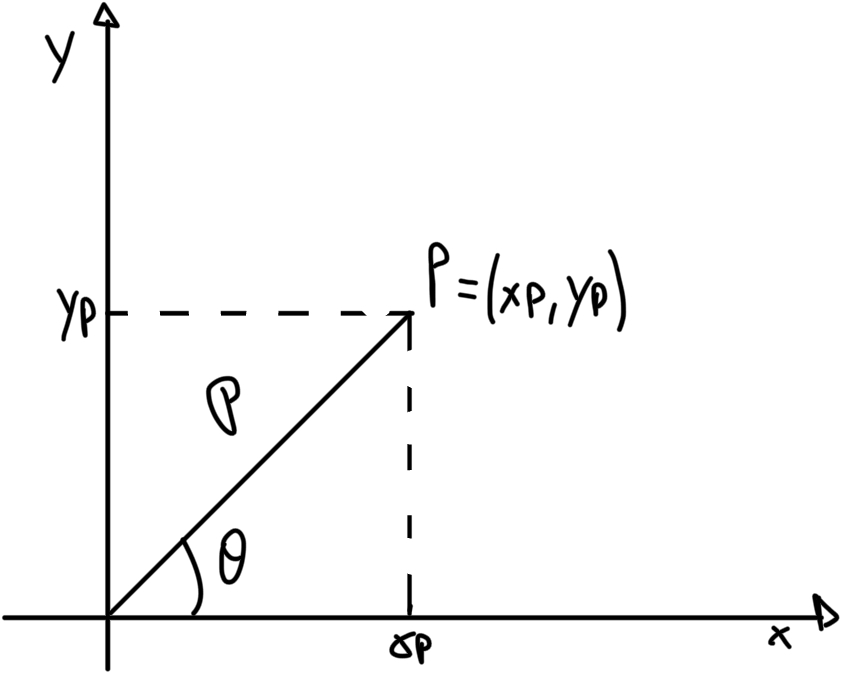
\includegraphics[width=0.5\textwidth]{Analisi2/figures/piano_coordinate_polari.jpeg}
    \caption{Grafico determinazione del punto $P=(x_P,y_P)$.}\label{fig:piano_coordinate_polari}
\end{figure}

\subsubsection{Coordinate polari}
\begin{definition}[Coordinate polari in $\mathbb R^2$ (non ufficiale)]\footnote{Slide 12, PDF 10.}\label{def:coordinate_polari}
    Siano $P=(x_P,y_P)\in\mathbb R^2$, $\rho=d(P,\uline 0)\in\mathbb R$ e $\theta$ l'angolo che $\overrightarrow{\rm OP}$ (orientato positivamente) forma con l'asse delle ascisse $x$. Data la circonferenza centrata nell'origine di raggio $\rho$, le coordinate polari di un punto $P$ nel piano $\mathbb R^2$ sono $(\rho, \theta)$, dove le coordinate polari sono determinate come
    \begin{equation}\label{eq:coordinate_polari_piano}
        \begin{cases}
            x_P=\rho\cos\theta\\
            y_P=\rho\sin\theta
        \end{cases}
    \end{equation}
\end{definition}

\begin{remark}\footnote{Slide 12 PDF 10.}
    Se $\rho\geq 0\Rightarrow \rho=\sqrt{x_P^2+y_P^2}$.
\end{remark}

\begin{remark}\footnote{Slide 12 PDF 10.}
    È possibile considerare la circonferenza trigonometrica centrata nell'origine di raggio $\rho$ come $\cos^2\theta+\sin^2\theta=\rho^2$. Quindi, l'ascissa è il coseno e l'ordinata il seno.
\end{remark}

\paragraph{N.B.:} Da (\ref{eq:coordinate_polari_piano}) è possibile dedurre che le coordinate cartesiane possono essere espresse in funzione delle coordinate polari. Quindi è necessario trovare $\theta$. Geometricamente $\theta$ è legata alla pendenza della retta $\overline{\rm OP}$ e la tangente di $\theta$ è il coefficiente angolare di $\overline{\rm OP}$. La pendenza può essere visualizzata come di quanto ci siamo alzati rispetto quanto ci siamo mossi, quindi $\frac{x}{y}$ (infatti $\tan x=\frac{\sin x}{\cos x}$). Quindi, se $\tan\theta$ è la pendenza di $\overline{\rm OP}$, 
\begin{equation*}
    \theta=\arctan\left(\frac{y_P}{x_P}\right).
\end{equation*}
Quindi la retta $\overline{\rm OP}$ può essere rappresentata come $y=mx$, con $m=\tan\theta$, dato che $\overline{\rm OP}$ passa per l'origine.

\begin{remark}[Non ufficiale]\footnote{Slide 13 PDF 10.}
    Le coordinate polari definite come nella Definizione \ref{def:coordinate_polari} sono centrate centrate in $(0,0)$. Le coordinate polari potrebbero essere traslate e centrate nel punto $(x_0,y_0)\neq(0,0)$ come in Figura \ref{fig:piano_coordinate_polari_centrate_x0_y0}, quindi è possibile generalizzare il caso (\ref{eq:coordinate_polari_piano}), ovvero: Nel caso in cui le coordinate siano centrate in $(x_0,y_0)$ allora $x$ e $y$ in coordinate cartesiano sono ottenute dalle coordinate polari seguendo le formule
    \begin{equation*}
        \begin{cases}
            x=x_0+\rho\cos\theta,\\
            y=y_0+\rho\sin\theta.
        \end{cases}
    \end{equation*}
\end{remark}
\begin{figure}
    \centering
    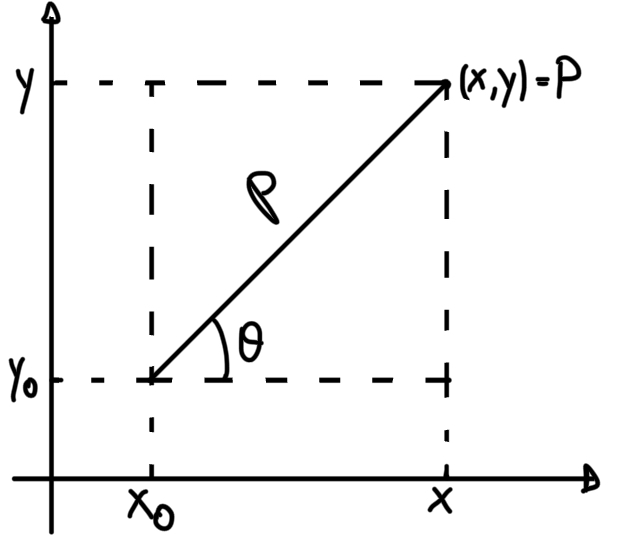
\includegraphics[width=0.5\textwidth]{Analisi2/figures/piano_coordinate_polari_centrate_x0_y0.jpg}
    \caption{Grafico determinazione del punto $P=(x,y)$.}\label{fig:piano_coordinate_polari_centrate_x0_y0}
\end{figure}

Il calcolo del limite di $f(P)$ quando $P\rightarrow P_0$ è possibile utilizzando le coordinate polari. Vale il seguente teorema.
\begin{theorem}\label{th:limite_funzione_due_variabili_coordinate_polari}\footnote{Slide 14 PDF 10.}
    Sia $f\colon D\subset\mathbb R^2\rightarrow\mathbb R$ e $P_0=(x_0,y_0)\in D$, allora
    \begin{equation}\label{eq:limite_tende_l_uniformemente_theta}
        \lim_{(x,y)\rightarrow(x_0,y_0)}f(x,y)=\ell\quad\iff\quad\lim_{\rho\rightarrow 0^+}\underbrace{f(x_0+\rho\cos\theta,y_0+\rho\sin\theta)}_{\footnotemark}=\ell\quad\text{$\underset{\footnotemark}{\text{uniformemente}}$ rispetto a $\theta$}.
    \end{equation}
\end{theorem}
\addtocounter{footnote}{-1}
\footnotetext{Dipende da $\rho$ e non da $\theta$ perché il limite deve valere uniformemente rispetto a $\theta$. È controllato quando $\rho\rightarrow0^+$ perché $\rho$ è una distanza, quindi $\rho\geq 0$.}

\stepcounter{footnote}
\footnotetext{Uniformemente rispetto a $\theta$ significa che il valore del limite cale comunque scelto $\theta$. È necessario ricordarsi che $\theta$ è un angolo, quindi di periodo $[0,2\pi]$ ed è sufficiente verificare cosa accade in tale intervallo e non su tutto $\mathbb R$.}

\paragraph{N.B.:} Nel caso del cambiamento di coordinate di una funzione, questa deve essere invertibile, quindi biettiva e per questo è necessario che il dominio della funzione sia un aperto (così ogni punto del dominio è associato ad un punto del codominio).

\paragraph{Conseguenze del Teorema \ref{th:limite_funzione_due_variabili_coordinate_polari}:} È valutato cosa accade quando $P=(x,y)\rightarrow P_0=(x_0,y_0)$. Con trasformazioni in coordinati polari del tipo
\begin{equation*}
    \begin{cases}
        x=x_0+\rho\cos\theta,\\
        y=y_0+\rho\sin\theta.
    \end{cases}
\end{equation*}
se $(x,y)\rightarrow(x_0,y_0)$ allora $\rho\cos\theta\rightarrow 0$ e $\rho\sin\theta\rightarrow 0$. Ciò vale per $\rho\rightarrow 0$ indipendentemente dal valore di $\theta\in(0,2\pi)$ ed è per questo che il limite (\ref{eq:limite_tende_l_uniformemente_theta}) vale uniformemente rispetto a $\theta$.\\
È utile passare in coordinate polari quando questo semplifica il calcolo dei limiti di funzioni radiali.

\paragraph{Cosa significa che $\boldsymbol{\lim_{\rho\rightarrow0^+}f(x_0+\rho\cos\theta, y_0+\rho\cos\theta)=\ell}$ (ovvero che vale (\ref{eq:limite_tende_l_uniformemente_theta}))?}

\begin{remark}[Non ufficiale]\footnote{Slide 1 PDF 11.}
    Affermare che vale il limite (\ref{eq:limite_tende_l_uniformemente_theta}) significa, tramite la Definizione \ref{def:limite_epsilon_delta} di limite $\varepsilon$-$\delta$, che
    \begin{equation}\label{eq:limite_coordinate_polari}
        \forall\varepsilon>0\; \exists\delta=\delta(\varepsilon)>0\quad\text{tc}\quad \underbrace{|f(x_0+\rho\cos\theta,y_0+\sin\theta)-\ell|}_{d(f(x_0, y_0),\ell)}<\varepsilon\quad\forall\rho\,(\rho\rightarrow0^+)\;0<\rho<\delta,\forall\theta\in(0,2\pi).
    \end{equation}
\end{remark}

\paragraph{N.B.:} Data l'Osservazione precedente, per mostrare che vale il limite della funzione $f$ per $(x,y)\rightarrow (x_0,y_0)$ è utilizzata un condizione semplice, ovvero è applicato il Teorema \ref{th:dei_carabinieri_2} dei Carabinieri: si cerca di maggiorare la quantità $|f(x_0+\rho\cos\theta,y_0+\sin\theta)-\ell|<\varepsilon$ in (\ref{eq:limite_coordinate_polari}) con una funzione che dipende solo dal raggio radiale, dove la funzione radiale è una maggiore uguale a 0 ed infinitesima (ovvero tende a 0 quando $\rho\rightarrow 0$).\\
Quindi, per mostrare che vale (\ref{eq:limite_tende_l_uniformemente_theta}) è sufficiente mostrare che (esiste) una funzione (radiale) $g=g(\rho)$ che dipende soltanto da $\rho$ con $g(\rho)\geq 0$ \footnote{Tale che $g$ sia maggiore di $|f(x_0+\rho\cos\theta,y_0+\sin\theta)-\ell|$ ed infinitesima quando $\rho\rightarrow 0^+$. Quindi è sufficiente far vedere che $g$ esiste, che sia maggiore uguale a 0 ed infinitesima quando $\rho\rightarrow 0^+$.} tale che
\begin{equation}\label{eq:maggiorazione_f_coordinate_polari}
    d(f,l)=|f(x_0+\rho\cos\theta,y_0+\sin\theta)-\ell|\leq g(\rho)\quad\text{e}\quad\lim_{\rho\rightarrow 0^+}g(\rho)=0.
\end{equation}
Quindi, (\ref{eq:maggiorazione_f_coordinate_polari}) significa che $d(f,\ell)$ è infinitesima non appena $0<\rho<\delta$, comunque scelta $\delta$.\\
Quindi, la tesi (\ref{eq:limite_tende_l_uniformemente_theta}) segue dal Teorema \ref{th:dei_carabinieri_2} dei Carabinieri (anche detto del confronto).

\paragraph{N.B.:} Potrebbe capitare che passando in coordinate polari il limite dipenda esplicitamente da $\theta$, ciò significa che il limite non esiste perché non vale uniformemente rispetto a $\theta$. Inoltre, se non riusciamo a dimostrare che esiste una $g\geq 0$ infinitesima per la quale vale la maggiorazione (\ref{eq:maggiorazione_f_coordinate_polari}), è necessario cercare un'altra strada.

\begin{example}\footnote{Slide 2 PDF 11.}
    È già stato visto per l'Esercizio \ref{exercise:limite_non_esiste_casa} che il seguente limite non esiste:
    \begin{equation*}
        \lim_{(x,y)\rightarrow(0,0)}\frac{xy}{x^2+y^2}.
    \end{equation*}
    Passando in coordinate polari (quando $(x,y)\rightarrow(0,0)$ e $\rho\rightarrow 0^+$)
    \begin{equation*}
        \begin{cases}
            x=\rho\cos\theta\\
            y=\rho\sin\theta
        \end{cases}
    \end{equation*}
    allora 
    \begin{equation*}
        \lim_{\rho\rightarrow 0^+}\frac{\rho\cos\theta\;\rho\sin\theta}{\underbrace{\rho^2\cos^2\theta+\rho^2\sin^2\theta}_{\rho^2\underbrace{(\cos^2\theta+\sin^2\theta)}_{1}}}\overset{\footnotemark}{=}\lim_{\rho\rightarrow 0^+}\frac{\rho^2\cos\theta\sin\theta}{\rho^2}=\cos\theta\sin\theta=\frac{1}{2}\sin(2\theta).
    \end{equation*}
    Quindi, il limite non esiste perché non uniforme al variare di $\theta$ (ovvero il limite dipende da $\theta$).
\end{example}
\footnotetext{Prima regola fondamentale della trigonometria.}

\begin{example}\footnote{Slide 2 PDF 11.}
    Risolvere
    \begin{equation*}
        \lim_{(x,y)\rightarrow(0,0)}\frac{xy}{\sqrt{x^2+y^2}}.
    \end{equation*}
    Passando in coordinate polari, allora
    \begin{equation*}
        \lim_{\rho\rightarrow 0^+}\frac{\rho^2\cos\theta\;\rho\sin\theta}{\sqrt{\rho^2\cos^2\theta+\rho^2\sin^2\theta}}\overset{\footnotemark}{=}\lim_{\rho\rightarrow 0^+}\frac{\rho^2\cos\theta\sin\theta}{\sqrt{\rho^2}}=\lim_{\rho\rightarrow 0^+}\frac{\rho^{\cancel{2}}\cos\theta\sin\theta}{\cancel{\rho}}=\lim_{\rho\rightarrow 0^+}\rho\cos\theta\sin\theta=0(=l).
    \end{equation*}
    $\rho\cos\theta\sin\theta\overset{\rho\rightarrow0^+}{=}0$ perché, utilizzando il teorema del confronto, $\rho\cos\theta\sin\theta$ è maggiorata da una \gls{funzione infinitesima}, ovvero:
    \begin{equation*}
        \rho\cos\theta\sin\theta\leq\underbrace{|\rho\cos\theta\sin\theta|}_{\rho\cos\theta\sin\theta-0=d(f,l)}=\left|\rho\frac{1}{2}\sin\theta\right|<\frac{1}{2}\rho,
    \end{equation*}
    dove $\frac{1}{2}\rho$ è una funzione infinitesima perché tende a 0 quando $\rho\rightarrow 0^+$.
\end{example}
\footnotetext{Come nell'esempio precedente $\rho^2\cos^2\theta+\rho^2\sin^2\theta=\rho^2(\cos^2\theta+\sin^2\theta)=\rho^2\cdot 1$ per la prima regola fondamentale della trigonometria.}

\paragraph{Quando è utile passare in coordinate polari?} Quando la funzione è radiale, quando sono presenti $x^2$ e $y^2$, prodotti tra incognite ed è possibile sfruttare al meglio le proprietà di tali coordinate (ad esempio le regole fondamentali della trigonometria).

\begin{example}\footnote{Slide 4 PDF 11.}
    Calcolare, se esiste
    \begin{equation*}
        \lim_{(x,y)\rightarrow(0,0)}\frac{(x+y)^2}{x^2+y^2}.
    \end{equation*}
    Passando in coordinate polari,
    \begin{equation*}
        \begin{matrix}
            \lim_{\rho\rightarrow 0^+}\frac{(\rho\cos\theta+\rho\sin\theta)^2}{\rho^2}&=&\lim_{\rho\rightarrow 0^+}\frac{\rho^2\cos^2\rho+\rho^2\sin^2\theta+2\rho^2\cos\theta\sin\theta}{\rho^2}&=& 1^a\text{ relazione fond. aritmetica}\\
            &=&\lim_{\rho\rightarrow0^+}\frac{\rho^2+2\rho^2\cos\theta\sin\theta}{\rho^2}&=&\lim_{\rho\rightarrow0^+}\frac{\cancel{\rho}^2(1+2\cos\theta\sin\theta)}{\cancel{\rho^2}},
        \end{matrix}
    \end{equation*}
    dipende da $\theta$, quindi il limite non esiste.
\end{example}

\begin{example}\footnote{Slide 4 PDF 11.}
    Studiare al variare del parametro $\alpha>0$ l'esistenza del seguente limite (il quale è una forma indeterminata)
    \begin{equation*}
        \lim_{(x,y)\rightarrow(1,0)}\frac{(x^2-2x+1)y}{(x^2-2x+1+y^2)^\alpha}=\lim_{(x,y)\rightarrow(1,0)}\frac{(x-1)^2y}{[(x-1)^2+y^2]^\alpha}.
    \end{equation*}
    Passando in coordinate polari
    \begin{equation*}
        \begin{cases}
            x=1+\rho\cos\theta\\
            y=\rho\sin\theta
        \end{cases}\Longrightarrow 
        \begin{cases}
            x-1=\rho\cos\theta\\
            y=\rho\sin\theta
        \end{cases}
    \end{equation*}
    allora
    \begin{equation*}
        \lim_{\rho\rightarrow0^+}\frac{\rho^2\cos^2\theta\rho\sin\theta}{[\rho^2\cos^2\theta+\rho^2\sin^2\theta]^\alpha}\overset{\footnotemark}{=}\lim_{\rho\rightarrow 0^+}\frac{\rho^3\cos^2\theta\sin\theta}{\rho^{2\alpha}}\overset{\text{prop. potenze}}{=}\lim_{\rho\rightarrow 0^+}\rho^{3-2\alpha}\cos^2\theta\sin\theta=0
    \end{equation*}
    in quanto $\rho^b\underset{\rho\rightarrow0^+}{\longrightarrow}0\;\forall b>0$.\\
    Poiché ($\cos^2\theta\sin\theta$ uniformemente limitata e minore di 0, è considerato l'estremo superiore di $\theta$)
    \begin{equation*}
        |\cos^2\theta\sin\theta|\leq 1\quad\text{se}\quad 3-2\alpha>0\equiv3>2\alpha\quad\text{ovvero}\quad 0\underset{\text{HP}\, \alpha>0}{<}\alpha<\frac{3}{2}\quad\text{allora}\quad 0<|\rho\cos^2\theta\sin\theta|<\rho^{3-2\alpha},
    \end{equation*}
    il limite vale 0 (per il Teorema \ref{th:dei_carabinieri_2} dei Carabinieri).\\
    Se $\alpha=\frac{3}{2}$ il limite dipende da $\theta$ (perché è il limite di $\cos^3\theta\sin\theta$), quindi non esiste.\\
    Se $3-2\alpha<0$, allora
    \begin{equation*}
        \lim_{\rho\rightarrow0^+}\rho^{3-2\alpha}\cos^2\theta\sin\theta=\lim_{\rho\rightarrow0^+}\frac{\cos^2\theta\sin\theta}{\rho^{2\alpha-3}}=\lim_{\rho\rightarrow0^+}\underbrace{\frac{1}{\rho^{2\alpha-3}}}_{+\infty}\cos^2\theta\sin\theta.
    \end{equation*}
    Quindi non esiste perché il segno dipende da $\theta$.
\end{example}
\footnotetext{Prima relazione fondamentale della trigonometria: $\rho^2\cos^2\theta+\rho^2\sin^2\theta=\rho^2(\cos^2\theta+\sin^2\theta)=\rho^2\cdot 1$.}

\subsection{Grafico di una funzione di più variabili}\label{ssec:grafico_funzione_n_variabili}
Per comodità (legata al grafico delle funzioni) sono considerate funzioni di due variabili, quindi del tipo
\begin{equation*}
	f : D\subseteq\mathbb R^2\rightarrow\mathbb R.
\end{equation*}
È possibile generalizzare su $\mathbb R^n$.

\begin{definition}[(Non ufficiale) Campo di esistenza in $\mathbb R^2$]\footnote{Slide 6 PDF 11.}
    Il campo di esistenza per le funzioni in 2 variabili è un sottoinsieme del piano ($\mathbb R^2$), per il quale l'espressione della funzione ha senso (ovvero assume valore reali).
\end{definition}

Il campo di esistenza può essere chiamato anche insieme di esistenza o insieme di definizione. Campo di esistenza e dominio possono coincidere, il dominio è un sottoinsieme del campo di esistenza.

\begin{remark}[Non ufficiale]
    Trovare il campo di esistenza di una funzione significa trovare l'insieme massimale rispetto all'inclusione su $\mathbb R^2$.
\end{remark}

\paragraph{N.B.:} Una funzione è un oggetto costituito da 3 elementi: dominio, codominio ed una legge. Ovvero:
\begin{equation*}
    \forall(x,y)\in D\;\exists!f(x,y)\in\mathbb R,
\end{equation*}
dove ad ogni punto di $D$ è associato un unico reale $f(x,y)$ appartenente al codominio.

Ricercare il dominio significa che è necessario trovare i punti del piano per cui l'espressione con la quale la funzione è descritta ha un significa. Per determinare il campo di esistenza in due variabili è spesso necessario risolvere equazioni (esempio rette) oppure disequazioni nelle due variabili.

\begin{definition}[Immagine di $f$]\footnote{Slide 6 PDF 11.}
    Sia $\forall(x,y)\in D\subseteq\mathbb R^2\;\exists!f(x,y)\in\mathbb R$. L'immagine di $f$ è
    \begin{equation*}
        Im(f)=graf\, f=\{z\in\mathbb R| f(x,y)=z,\,\forall(x,y)\in D\}\subseteq\mathbb R.
    \end{equation*}
\end{definition}

\paragraph{Cosa significa trovare insiemi di definizione?} Seguono alcuni esempi.
\begin{example}
    Sia $f(x,y)=5x+7y+11$. $f$ è ben definita $\forall(x,y)\in\mathbb R^2$, quindi $f\colon D=\mathbb R^2\rightarrow \mathbb R$.
\end{example}

\begin{example}\footnote{Slide 7 PDF 11.}
    Sia $f(x,y)=\frac{\log(x+y)}{x-4}$. $D=\{(x,y)\in\mathbb R^2\;;\; x+y>0,\, x\neq 4\}=\{(x,y)\in\mathbb R^2\;;\; x>-y,\, x\neq 4\}.$ $x+y=0$ è una retta che divide il piano in due.
    Vedere Figura \ref{fig:dominio_log(x+y)_x-4}.
    \begin{figure}
    \centering
        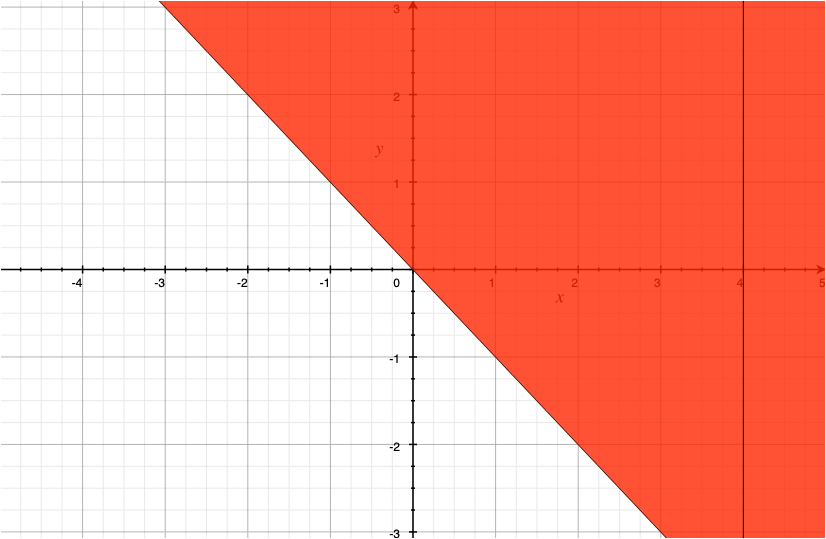
\includegraphics[width=0.5\textwidth]{Analisi2/figures/dominio_log(x+y)_x-4.jpg}
        \caption{Grafico di $D=\{(x,y)\in\mathbb R^2\;;\; x+y>0,\, x\neq 4\}$.}\label{fig:dominio_log(x+y)_x-4}
    \end{figure}
\end{example}

\begin{remark}[Non ufficiale]\footnote{Slide 8 PDF 11.}
    Per le funzioni di una o di più variabili il grafico è un sottoinsieme dello spazio in $n+1$ dimensioni. Quindi, per le funzioni in due variabili il grafico è l'insieme di terne $(x,y,z)$ tale per cui $z=f(x,y)$ con $(x,y)\in D$, ovvero: data $f\colon I\subseteq\mathbb R^2\rightarrow\mathbb R,\quad graf\;f =\{(x,y,z)\in\mathbb R^3\;;\;(x,y)\in D,\, z=f(x,y)\}\subseteq\mathbb R^3$. Per una funzione di una variabile $f\colon I\subseteq\mathbb R\rightarrow\mathbb R,\; graf\;f =\{(x,y)\in\mathbb R^2\;;\; y=f(x),\, \forall x\in I\}\subseteq\mathbb R^2$.
\end{remark}

\paragraph{N.B.:} \textbf{Sarà trattato solo il grafico di funzioni in due variabili perché oltre non $\boldsymbol n$ dimensioni è possibile rappresentarlo. Non è possibile rappresentare un grafico di una funzione in tre variabili perché sarebbe in 4 dimensioni, e così via.}

\paragraph{N.B.:} Per rappresentare il grafico di una funzione in 2 variabili, ovvero un sottoinsieme di $\mathbb R^3$, sono utilizzate le sezioni. Le sezioni tagliano il grafico con dei piano paralleli agli assi coordinati. Ad esempio: fissato $z=k$, il grafico è affettato ad altezza $k$ ed è intersecato con il piano $(x,y)$. Se $x=k$ il grafico è intersecato con il piano $(y,z)$. Se $y=k$, il grafico è intersecato con il piano $(x,z)$. Quindi, utilizzando le sezioni, il grafico non è più in $\mathbb R^3$ ma in $\mathbb R^2$.

\paragraph{N.B.:} Sarà trattato il grafico delle funzioni in due variabili utilizzando il concetto geometrico di sezione di insieme. Ovvero, è affettato il grafico in $\mathbb R^3$ in un piano $z$ costante diminuendo la dimensione del problema ad $\mathbb R^2$ tracciando delle sezioni del grafico in $\mathbb R^3$ nei piani
\begin{equation}\label{eq:piani}
    \begin{matrix}
        x=k\\
        y=k\\
        z=k
    \end{matrix}
\end{equation}

%slide 8 PDF 11
\begin{figure}
\centering
    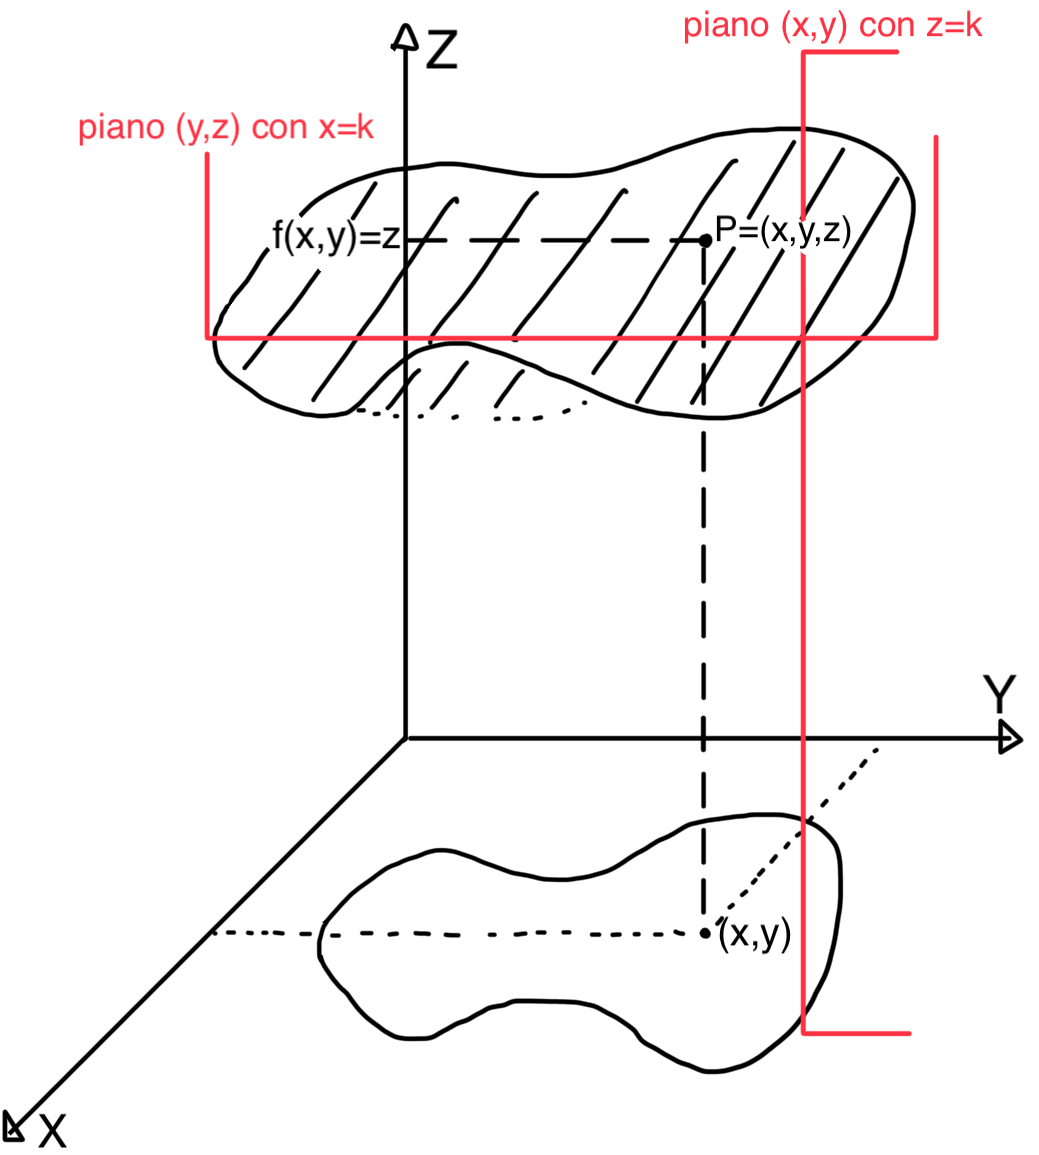
\includegraphics[width=0.75\textwidth]{Analisi2/figures/grafico_f_generica_R3.jpg}
    \caption{Grafico di $f$ funzione in due variabili.}\label{fig:grafico_f_generica_R3}
\end{figure}

Se intersecato il grafico con i piani (\ref{eq:piani}) (vedere Figura \ref{fig:grafico_f_generica_R3}) sono ottenute le sezioni trasversali del grafico. è utile utilizzare le sezioni per abbassare la dimensione del problema.

Considerato il grafico di $f$ definita in $\mathbb R^2$, questo è l'insieme di terne $(x,y,z)$. Considerate le sezioni è come se il grafico fosse tagliato con i piani $x=k,\, y=k,\, z=k$, dove $k\in\mathbb R$ è una costante. Ad esempio, con il seguente sistema è ottenuta l'intersezione del piano $y=k$ con il grafico di $f$ (sulle $y$)
\begin{equation*}
    \begin{cases}
        y=k\\
        z=f(x,y)
    \end{cases}\equiv
    \begin{cases}
        graf\,f\\
        y=k
    \end{cases}
\end{equation*}

\begin{example}\footnote{Slide 9 PDF 11.}\label{example:disegnare_tracce_x^2-y}
    Sia $f(x,y)=x^2-y$, dove $f\colon\mathbb R^2\rightarrow\mathbb R$. Disegnarne le tracce.\\
    $graf\,f=\{(x,y,z)\in\mathbb R^3,\, (x,y)\in\mathbb R^2,\, z=x^2-y\}$.\\
    Considerando la regione $x=k$ (ovvero l'intersezione del grafico con il piano $(y,z)$)
    \begin{equation}\label{eq:esempio_intersezione_piano_y_z}
        \begin{cases}
            graf\, f\\
            x=k
        \end{cases}\rightarrow
        \begin{cases}
            z=f(x,y)=f(k,y)\\
            x=k
        \end{cases}
    \end{equation}
    \footnotemark e dunque è ottenuto un insieme nel piano $(y,z)$
    \begin{equation}\label{eq:fascio_rette_nel_piano}
        \begin{cases}
            z=x^2-y\\
            x=k
        \end{cases}\longrightarrow z=-y+k^2\quad \forall k\in\mathbb R.
    \end{equation}
    Quindi $z$ è un fascio di rette parallele con coefficiente -1, vedere Figura \ref{fig:esempio_z=-y+k2}. \footnotemark\\
    Cambiando le regioni con $y=k$,
    \begin{equation}\label{eq:esempio_intersezione_piano_x_z}
        \begin{cases}
            graf\, f\\
            y=k
        \end{cases}\rightarrow
        \begin{cases}
            z=f(x,y)=f(x,k)\\
            y=k
        \end{cases}
    \end{equation}
    Tale regione (sezione) è un insieme nel piano $(x,z)$ che è dato dal grafico della funzione $z=f(x,k)$ nel piano $(x,z)$. (Ciò cosa significa? \footnotemark).\\
    (Quindi, se il grafico di $f$ è tagliato facendolo intersecare con il piano $(x,z)$ sono ottenute parabole, vedere Figura \ref{fig:esempio_z=x^2-k}, oppure se intersecato con il piano $(y,z)$ sono ottenute rette, vedere Figura \ref{fig:esempio_z=-y+k2}).\\
    Considerando la regione $z=k$,
    \begin{equation}\label{eq:esempio_intersezione_piano_x_y}
        \begin{cases}
            graf\, f\\
            z=k
        \end{cases}\rightarrow
        \begin{cases}
            z=f(x,y)=f(x,y)\\
            z=k
        \end{cases}
    \end{equation}
    il grafico è un oggetto è nel piano $(x,y)$ ed è formato dalle coppie $(x,y)\in D$ tali che $f(x,y)=k$, al variare di $k$ (Vedere Figura \ref{fig:esempio_z=k=x^2-y}).
\end{example}
\addtocounter{footnote}{-2}
\footnotetext{(\ref{eq:esempio_intersezione_piano_y_z}) rappresenta il grafico della funzione nel piano $(y,z)$, dove $z$ è in funzione di $y$ (ovvero $f$ è una funzione di una variabile). Osservando la Figura \ref{fig:grafico_f_generica_R3}, quando $y=k$, dove $k$ è una costante, significa che è tagliato il piano $(y,z)$ nel grafico di $f$ ed $f$ diventa in funzione di $y$. In modo analogo, se $x=k$, il piano del grafico è $(x,z)$. Inoltre, se $z=k$ allora il piano è $(x,y)$.}

\stepcounter{footnote}
\footnotetext{Nel piano $(x,y)$, quello disegnato in Figura \ref{fig:esempio_z=-y+k2}, è sezionato il grafico (in 3 dim.) della funzione con il piano $y=k$, trovando tutte le rette di pendenza $-1$ e parallele alla retta $z=-y$ (ovveo del tipo $z=-y+k^2$ in (\ref{eq:fascio_rette_nel_piano}).}

\stepcounter{footnote}
\footnotetext{(\ref{eq:esempio_intersezione_piano_x_z})$\equiv z=f(x,k)=x^2-k$, ovvero fasci di rette. Quindi, le sezioni del grafico di $f$ sono date da parabole, come descritto in Figura \ref{fig:esempio_z=x^2-k}. Il grafico di $f$ è in 3 dimensioni, ma se tagliato con $y=k$ è intersecato con il piano $(y,z)$.}

%slide 10 PDF 11
\begin{figure}
\centering
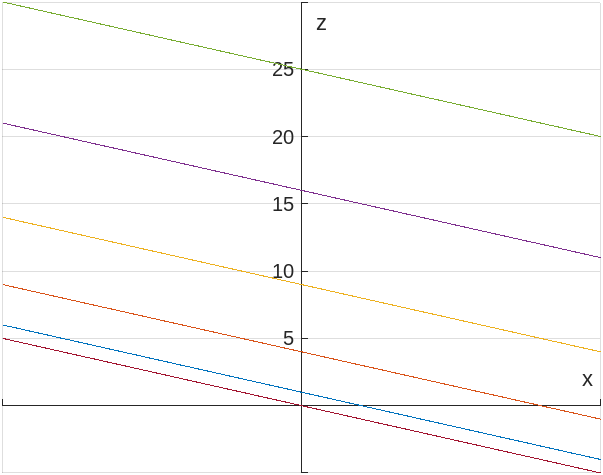
\includegraphics[width=0.5\textwidth]{Analisi2/figures/esempio_z=-y+k2.png}
    \caption{Grafico di $z=-y+k^2$, con $k\in[-5,5]\subset\mathbb N$ (nella realtà è $\forall k\in\mathbb R$).}\label{fig:esempio_z=-y+k2}
\end{figure}

\begin{figure}
\centering
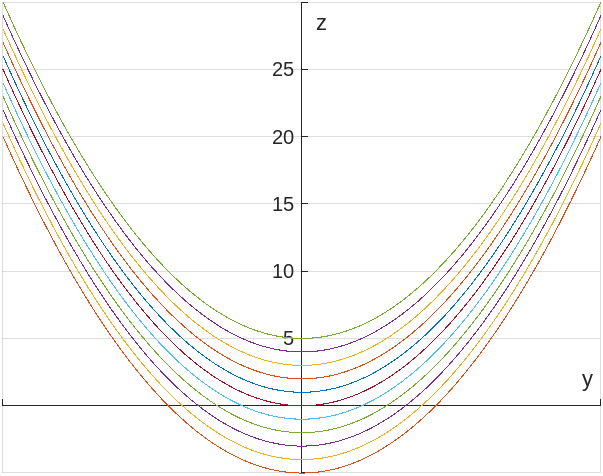
\includegraphics[width=0.5\textwidth]{Analisi2/figures/esempio_z=x^2-k.png}
    \caption{Grafico di $z=x^2-k$, con $k\in[-5,5]\subset\mathbb N$ (nella realtà è $\forall k\in\mathbb R$).}\label{fig:esempio_z=x^2-k}
\end{figure}

\begin{figure}
\centering
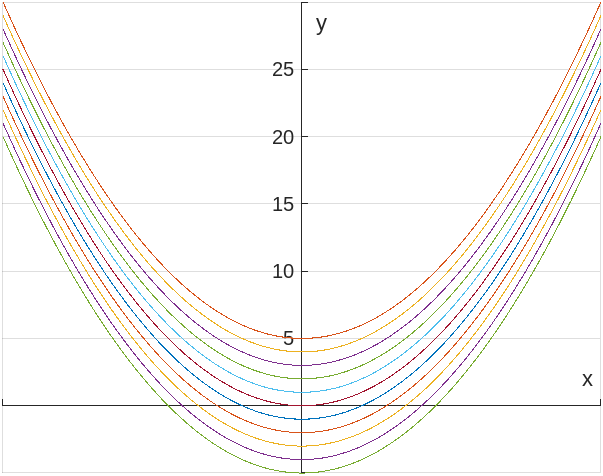
\includegraphics[width=0.5\textwidth]{Analisi2/figures/esempio_z=x^2-y.png}
    \caption{Grafico di $z=k=x^2-y$, con $k\in[-5,5]\subset\mathbb N$ (nella realtà è $\forall k\in\mathbb R$).}\label{fig:esempio_z=k=x^2-y}
\end{figure}

\paragraph{N.B.:} In Figura \ref{fig:esempio_z=k=x^2-y}, il paraboloide sezionato nel piano $(x,y)$ per $k\in\mathbb R$ avrà un oggetto nel dominio.

\begin{definition}[Insieme (o curve) di livello $k$]\footnote{Slide 12 PDF 11.}
    Data $f:D\subseteq\mathbb R^n\rightarrow\mathbb R$, l'insieme di livello $k$ è definito come
    \begin{equation}\label{eq:insime_livello_k_Rn}
        E_k=\{\uline x\in D\,|\, f(\uline x)=k,\, k\in\mathbb R\}\subset\mathbb R.
    \end{equation}
\end{definition}

\begin{remark}[Non ufficiale]
    Nel caso di funzioni di due variabili, l'insieme di livello $k$ è dato dagli elementi del dominio $(x,y)\in D$ tali che è risolto $f(x,y)=k$. Ciò si ha quando è considerata la regione $z=k$, quindi l'intersezione del grafico di $f$ con il piano $(x,y)$.
\end{remark}

\begin{remark}\footnote{Slide 8 PDF 14.}
    Se un insieme di livello $E_k$ ha livello $k$ non raggiungibile da $f$ allora $E_k=\emptyset$. Ad esempio, se $k<0$ e $f(x,y)=x^2+y^2$ allora $\nexists(x,y)\in\mathbb R^2$ tali che $f(x,y)=x^2+y^2=k$, quindi $E_k=\emptyset$.
\end{remark}

\paragraph{N.B.:} Gli insiemi (o curve) di livello sono chiamati così perché a volte rappresentano delle curve nel piano (esempio: carte topologiche).

\paragraph{N.B.:} Un insieme è detto di livello $k$ perché quando sono considerate le curve di livello sul piano $(x,y)$, per ottenere un grafico in $\mathbb R^3$ è sufficiente "tirare su" i punti attraverso la funzione. Questo perché il grafico di $f$ è dato da $z=f(x,y)$. In altre parole: preso un punto in $E_k$, è assegnata la quota $z$ e così è assegnato il punto nel grafico.

\begin{example}
    Sia l'Esempio \ref{example:disegnare_tracce_x^2-y}. Considerando $z=f(x,y)$ intersecato con $z=k$, l'insieme di livello $k$ è $E_k=\{(x,y)\in\mathbb R^2\,|\, x^2-y=k\}$.
\end{example}

\begin{exercise}\footnote{Slide 1 PDF 12.}
    Determinare l'insieme di definizione $E\subseteq\mathbb R^2$ della funzione
    \begin{equation*}
        f(x,y)=\frac{\log(x^3-y)}{\sqrt{1-xy}}.
    \end{equation*}
    \begin{equation*}
        \begin{matrix}
            E &=& \{(x,y)\in\mathbb R^2\,|\, x^3-y>0,\,\sqrt{1-xy}\neq 0,\, 1-xy> 0\} &=& \{(x,y)\in\mathbb R^2\,|\, y<x^3,\, 1-xy>0\}\\
            &=& \{(x,y)\in\mathbb R^2\,|\, y<x^3,\, xy-1<0\} &=&\{(x,y)\in\mathbb R^2\,|\, y<x^3,\, xy<1\}.
        \end{matrix}
    \end{equation*}
    $E$ è un illimitato e aperto.
    Vedere Figura \ref{fig:esempio_dominio_analisi2_1}.
    \begin{figure}
    \centering
    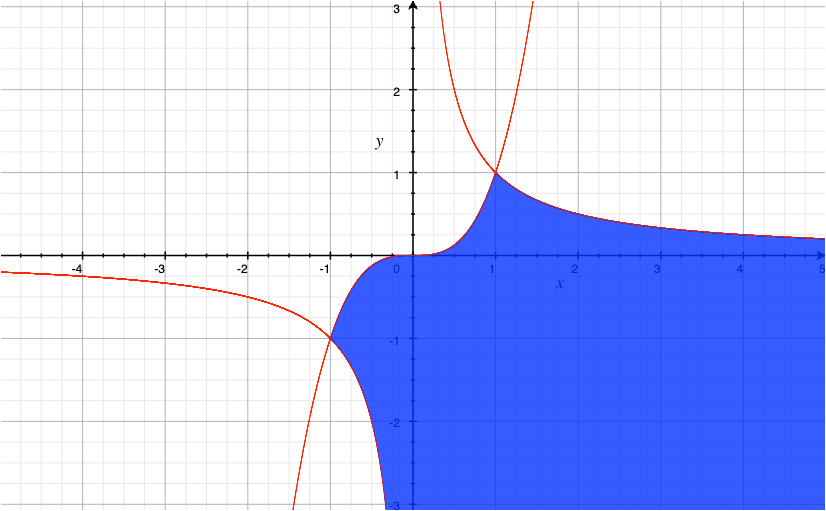
\includegraphics[width=0.65\textwidth]{Analisi2/figures/esempio_dominio_analisi2_1.jpg}
        \caption{Grafico di $E=\{(x,y)\in\mathbb R^2\,|\, x^3-y>0,\,\sqrt{1-xy}\neq 0,\, 1-xy\geq 0\}=\{(x,y)\in\mathbb R^2\,|\, y<x^3,\, 1-xy>0\}$.}\label{fig:esempio_dominio_analisi2_1}
    \end{figure}
\end{exercise}

\begin{example}\footnote{Slide 8 PDF 12.}
    I punti $(x,y)\in\mathbb R^2$ che sono nell'insieme di livello $k=1$ della funzione $f(x,y)=x^2+y^2$ sono i punti che verificano $x^2+y^2=1$, ovvero:
    \begin{equation*}
        E_1=\{(x,y)\in\mathbb R^2\,|\, f(x,y)=1\}=B(\uline 0, 1).
    \end{equation*}
    Vedere Figura \ref{fig:E_1}.
    \begin{equation*}
        E_k=\{(x,y)\in\mathbb R^2\,|\, x^2+y^2=k\}.
    \end{equation*}
    \begin{enumerate}
        \item Se $k<0$ allora $E_k=\{(x,y)\in\mathbb R^2\,|\, x^2+y^2<k\}=\emptyset$,
        \item Se $k=0$ allora $E_0=\{(x,y)\in\mathbb R^2\,|\, x^2+y^2=0\}=\{(0,0)\}$,
        \item Se $k>0$ allora $E_k=\{(x,y)\in\mathbb R^2\,|\, x^2+y^2>k\}=B(\uline 0,\sqrt{k})$.
    \end{enumerate}
    Vedere Figura \ref{fig:E_k_2D} e Figura \ref{fig:E_k_3D}. La Figura \ref{fig:E_k_3D_1} fa vedere come le sezione "tirate su" disegnino il grafico di $f(x,y)=x^2+y^2$.
    
    \begin{figure}
    \centering
    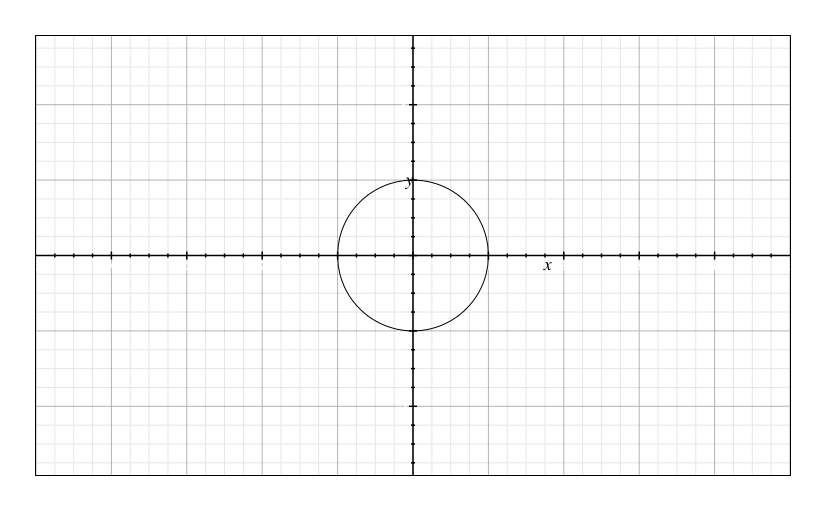
\includegraphics[width=0.65\textwidth]{Analisi2/figures/E_1.jpg}
        \caption{Grafico di $E_1=\{(x,y)\in\mathbb R^2\,|\, f(x,y)=1\}=B(\uline 0, 1)$.}\label{fig:E_1}
    \end{figure}
    
    \begin{figure}
    \centering
    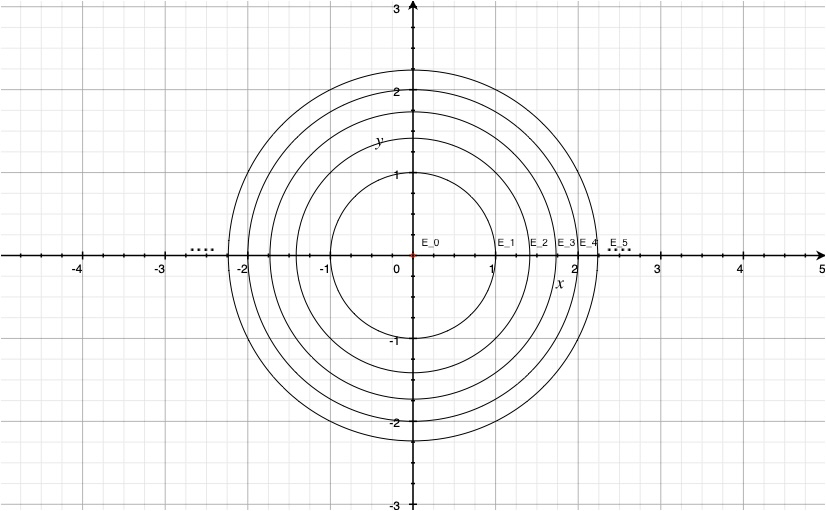
\includegraphics[width=0.65\textwidth]{Analisi2/figures/E_k_2D.jpg}
        \caption{Grafico di $E_k=\{(x,y)\in\mathbb R^2\,|\, x^2+y^2=k\}=B(\uline 0, \sqrt{k})$.}\label{fig:E_k_2D}
    \end{figure}
    
    \begin{figure}
    \centering
    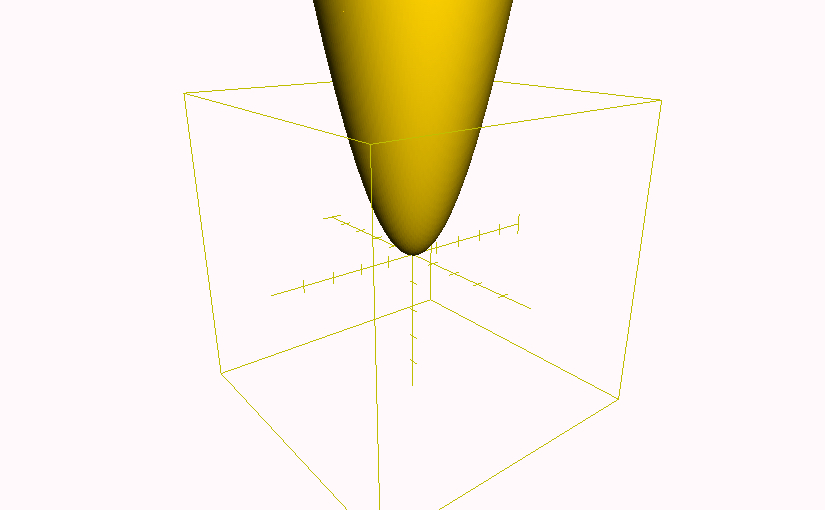
\includegraphics[width=0.65\textwidth]{Analisi2/figures/E_k_3D.jpg}
        \caption{Grafico di $z=f(x,y)=x^2+y^2$.}\label{fig:E_k_3D}
    \end{figure}
    
    \begin{figure}
    \centering
    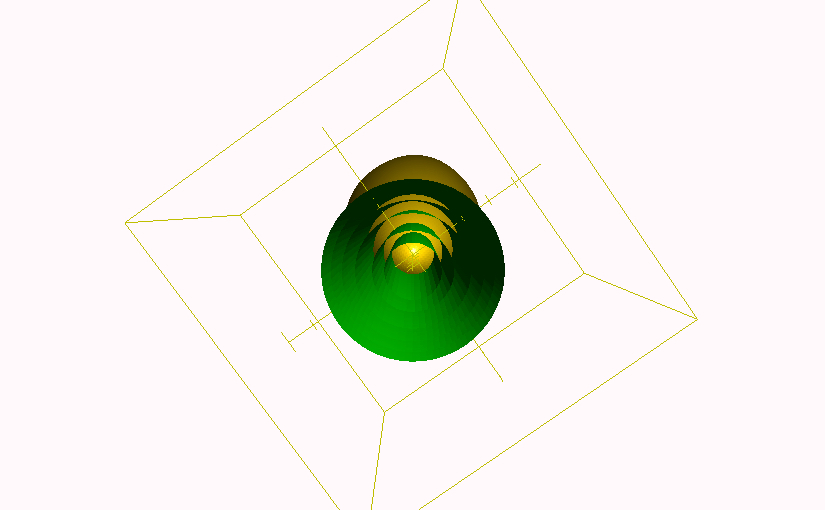
\includegraphics[width=0.65\textwidth]{Analisi2/figures/E_k_3D_1.jpg}
        \caption{Grafico di $z=f(x,y)=x^2+y^2$ intersecato con $E_k$.}\label{fig:E_k_3D_1}
    \end{figure}
\end{example}

\begin{example}\footnote{Slide 13-15 PDF 12.}
    Disegnare l'insieme di livello $E_k$ delle seguenti funzioni $f\colon E\subseteq\mathbb R^2\rightarrow\mathbb R$:
    \begin{enumerate}
        \item (per casa) $z=x+2y$.
        \item $z=x^2+9y^2$.
        \begin{equation*}
            E_k=\{(x,y)\in\mathbb R^2\,|\,x^2+9y^2=k\}.
        \end{equation*}
        \begin{itemize}
            \item $k<0\Longrightarrow E_k=\emptyset$,
            \item $k=0 \Longrightarrow E_k=\{(0,0)\}$,
            \item $k>0$ \footnote{Quando $k>0$ allora $x^2+9y^2=k$ rappresenta un'ellissi negli assi $(x,y)$. Un ellisse di semiassi $a$ e $b$ ha la forma in Figura \ref{fig:esempio_ellisse} ed è espresso come (\ref{eq:ellisse_assi_a,b}). È necessario portare l'ellisse in una forma conosciuta, ovvero in forma (\ref{eq:ellisse_assi_x,y}) (dai semiassi $(a,b)$ a $(x,y)$). La trasformazione da asse $(a,b)$ in asse $(x,y)$ è fatta  dividendo per $(\sqrt{x})^2=k$, il quale rappresenta $a^2$, e $\left(\sqrt{\frac{k}{2}}\right)^2$, il quale rappresenta $b^2$.} 
            \begin{equation}\label{eq:ellisse_assi_a,b}
                \frac{x^2}{a^2}+\frac{y^2}{b^2}=1
            \end{equation}
            allora
            \begin{equation}\label{eq:ellisse_assi_x,y}
                \frac{x^2}{\left(\sqrt{k}\right)^2}+\frac{y^2}{\left(\frac{\sqrt{k}}{3}\right)^2}=1.
            \end{equation}
            \begin{figure}
            \centering
            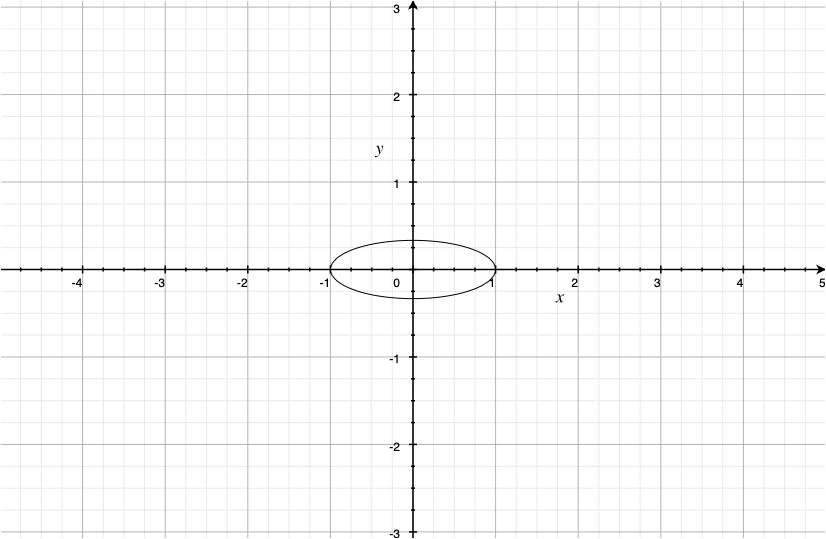
\includegraphics[width=0.5\textwidth]{Analisi2/figures/esempio_ellisse.jpg}
                \caption{Grafico di $f(x,y)=x^2+9y^2$.}\label{fig:esempio_ellisse}
            \end{figure}
        \end{itemize}
        \item $z=\frac{2x}{x^2+y^2}.\, f:E=\mathbb R^2\backslash\{(0,0)\}\rightarrow\mathbb R.$
        \begin{equation*}
            E_k=\left\{(x,y)\in E\,|\, \frac{2x}{x^2+y^2}=k\right\}.
        \end{equation*}
        \begin{itemize}
            \item Se $k=0\Rightarrow E_0=\left\{(x,y)\in E\,|\, \frac{2x}{x^2+y^2}=0\right\}=\{x=0, \text{ con } y\neq 0\},$
            \item Se $k\neq 0\Rightarrow E_k=\left\{(x,y)\in E\,|\, \frac{2x}{x^2+y^2}=k\right\}\Rightarrow\frac{2x}{x^2+y^2}=k\Rightarrow 2x=kx^2+ky^2\Rightarrow kx^2+ky^2-2x=0\Rightarrow$ con $\left(x-\frac{1}{k}\right)^2+y^2=\frac{1}{k^2 },\, \underbrace{x^2+y^2-\frac{2}{k}x=0}_{B\left(\left(\frac{1}{k},\, 0\right),\frac{1}{k}\right)}.$
        \end{itemize}
        \item $z=\frac{y}{x^2}.\, E=\left\{(x,y)\in\mathbb R^2\,|\, x\neq 0\right\}$ (unione di due semipiani).
        \begin{equation*}
            E_k=\left\{(x,y)\in E\,|\, \frac{y}{x^2}=k\right\}.
        \end{equation*}
        \begin{itemize}
            \item Se $k=0\Rightarrow E_0=\{y=0,\text{ con } x\neq 0\}$ (asse $x$ privata di $(0,0)$),
            \item $k>0 \Rightarrow E_k=\left\{(x,y)\in E\,|\, \frac{y}{x^2}=k\right\}=\{(x,y)\in E\,|\, y\overset{\footnotemark}{=}kx^2\}$ (parabola con vertice $V=(0,0)$ escluso e concavità verso l'alto),
            \item $k<0\Rightarrow E_k=\{(x,y)\in E\,|\, y=kx^2\}$ (parabola con vertice $V=(0,0)$ escluso e concavità verso il basso).
        \end{itemize}
        \begin{figure}
        \centering
        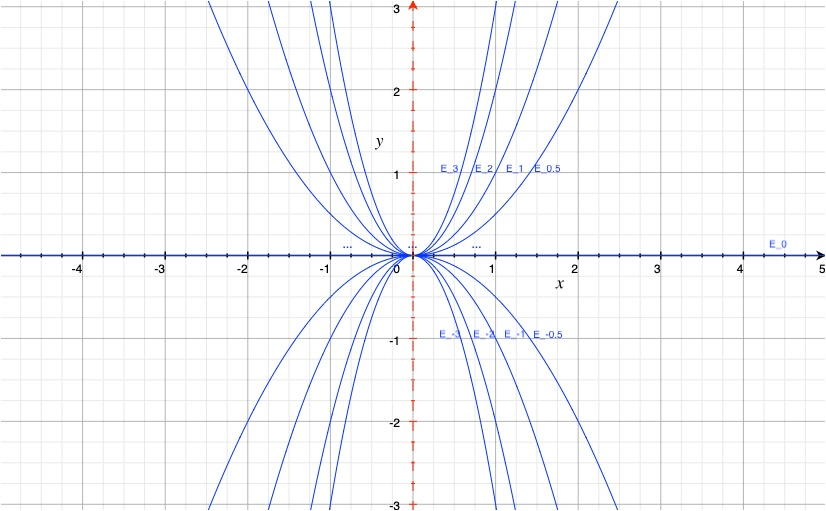
\includegraphics[width=0.65\textwidth]{Analisi2/figures/esempio_E_k.jpg}
            \caption{Grafico di $E_k=\left\{(x,y)\in E\,|\, \frac{y}{x^2}=k\right\}$ (asse $y$ escluso).}\label{fig:esempio_E_k}
        \end{figure}
    \end{enumerate}
\end{example}

\paragraph{Insiemi del piano determinati da equazioni o disequazioni (in due variabili)} La questione è legata alle proprietà di continuità delle funzioni in due variabili e alle funzioni in una variabile.\\
Sia $f\colon I=[a,b]\subseteq\mathbb R\rightarrow\mathbb R$ continua, dove grafico $graf\, f=\{(x,y)\in\mathbb R^2\,|\, y=f(x),\; x\in I\}\subseteq\mathbb R^2$ descrive una curva \footnotemark continua come in Figura \ref{fig:grafico_f_R2}. Sono date le definizioni di sotto/sopra/semigrafico (e sono valide anche con $<$ al posto di $\leq$).
\footnotetext{In matematica le curve sono operazioni definite da un intervallo ad un insieme, a seconda che le curve siano piane o nello spazio $\mathbb R^n$. Nel caso di Figura \ref{fig:grafico_f_R2} la curva è piana, dove è possibile pensarla come arco di curva continua.}

\begin{figure}
    \centering
    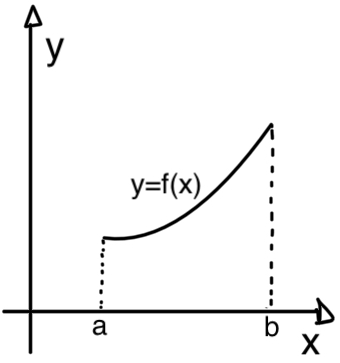
\includegraphics[width=0.5\textwidth]{Analisi2/figures/grafico_f_R2}
        \caption{Grafico di $y=f(x)$.}\label{fig:grafico_f_R2}
\end{figure}

\begin{definition}[Sottografico]\footnote{Slide 2 PDF 12.}
    Il sottografico di $f$ è definito come
    \begin{equation*}
        \{(x,y)\in\mathbb R^2\,|\, y\leq f(x),\, x\in I\}\subseteq\mathbb R^2.
    \end{equation*}
    Vedere Figura \ref{fig:sottografico_f_R2}.
\end{definition}
\begin{definition}[Sopragrafico]\footnote{Slide 3 PDF 12.}
    Il sopragrafico di $f$ è definito come
    \begin{equation*}
        \{(x,y)\in\mathbb R^2\,|\, y\geq f(x),\, x\in I\}\subseteq\mathbb R^2.
    \end{equation*}
    Vedere Figura \ref{fig:sopragrafico_f_R2}.
\end{definition}

\begin{definition}[Semipiano]\footnote{Slide 3 PDF 12.}
    Un semipiano è determinato da una equazione di grado 1.
\end{definition}

\begin{figure}
    \centering
    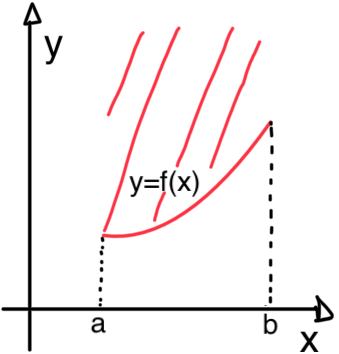
\includegraphics[width=0.5\textwidth]{Analisi2/figures/sopragrafico_f_R2.jpg}
        \caption{Sopragrafico di $y=f(x)$.}\label{fig:sopragrafico_f_R2}
\end{figure}

\begin{figure}
    \centering
    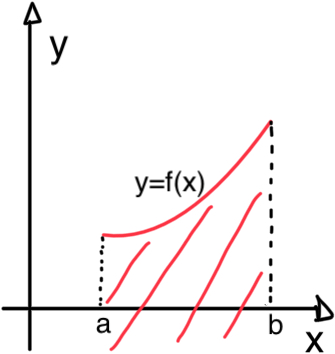
\includegraphics[width=0.5\textwidth]{Analisi2/figures/sottografico_f_R2.jpg}
        \caption{Sottografico di $y=f(x)$.}\label{fig:sottografico_f_R2}
\end{figure}

\begin{example}\footnote{Slide 4 PDF 12.}
    Sia $2x-3y+1\geq 0$. $2x-3y+1=0$ è una retta ed un semipiano, in quanto $3y=2x+1$, ovvero $y=\frac{2x+1}{3}$. Quindi, la disequazione è il sottografico della retta (per $-3y$). Vedere Figura \ref{fig:esempio_sottografico}.
    \begin{figure}
    \centering
    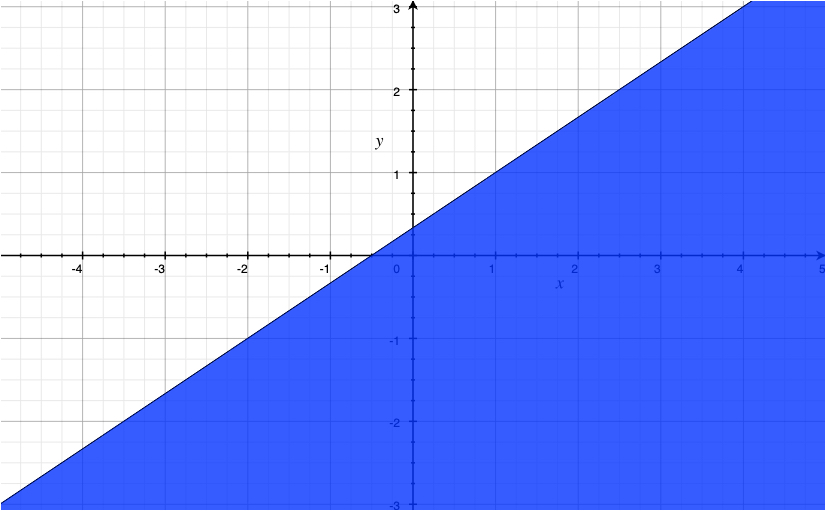
\includegraphics[width=0.5\textwidth]{Analisi2/figures/esempio_sottografico.jpg}
        \caption{Sottografico di $2x-3y+1=0$.}\label{fig:esempio_sottografico}
    \end{figure}
\end{example}

\begin{example}\footnote{Slide 4 PDF 12.}
    Trovare i punti del piano per i quali  è verificata la disequazione
    \begin{equation}\label{eq:esempio_disequazione}
        x^2-y^2\geq 1.
    \end{equation}
    Definita $f(x,y)=x^2-y^2-1$, una funzione continua $\forall(x,y)\in\mathbb R^2$, allora la disequazione (\ref{eq:esempio_disequazione}) è equivalente a $f(x,y)\geq 0$.
    
    Consideriamo cosa accade quando $f(x,y)=0$, ovvero consideriamo l'insieme di punti sottoinsieme di $\mathbb R^2$ tali che $x^2-y^2-1=0$ (ovvero, l'iperbole traslata passante in $\pm 1$ sia uguale a 0).
    Vedere Figura \ref{fig:grafico_x^2-y^2-1}. $f(x,y)$ divide il piano in 3 zone illimitate, ovvero 3 insiemi aperti e connessi: $A_1,\, A_2,\, A_3$ nei quali $f(x,y)\neq 0$ ed è continua. In ciascuna delle 3 regioni il segno non cambia \footnote{Il segno non cambia perché in ognuna di esse $f\neq 0$ ed è continua. Ciò significa che per mostrare quanto vale il segno di $f$ in ogni zona è sufficiente calcolarla in un punto comodo. I punti comodi interessanti nell'esempio sono l'origine perché in $A_2$, $(2,0)$ perché in $A_3$ e $(-2,0)$ perché in $A_1$.}
    \begin{itemize}
        \item $f(0,0)=-1<0,\quad f(x,y)<0\;\forall (x,y)\in A_2$,
        \item $f(2,0)=4-1=3>0\quad f(x,y)>0\; \forall (x,y)\in A_3$,
        \item $f(-2,0)=4-1=3>0\quad f(x,y)>0\; \forall (x,y)\in A_1$.
    \end{itemize}
    
    Nelle tre regioni $f$ ha segno costante ed è continua, quindi dove è diversa da 0 $f$ ha l'insieme immagine formata da un aperto (in questo caso l'unione di aperti) connesso.

    Essendo il segno 0 nelle due parabole, questo cambia passando fra $A_1,\, A_2$ e $A_3$. Ovvero: in $A_1$ e $A_3$ il segno è positivo ed in $A_2$ il segno è negativo, quindi \uline{vale il Teorema \ref{th:esistenza_degli_zeri} degli zeri in più dimensioni}.
    
    \begin{figure}
    \centering
    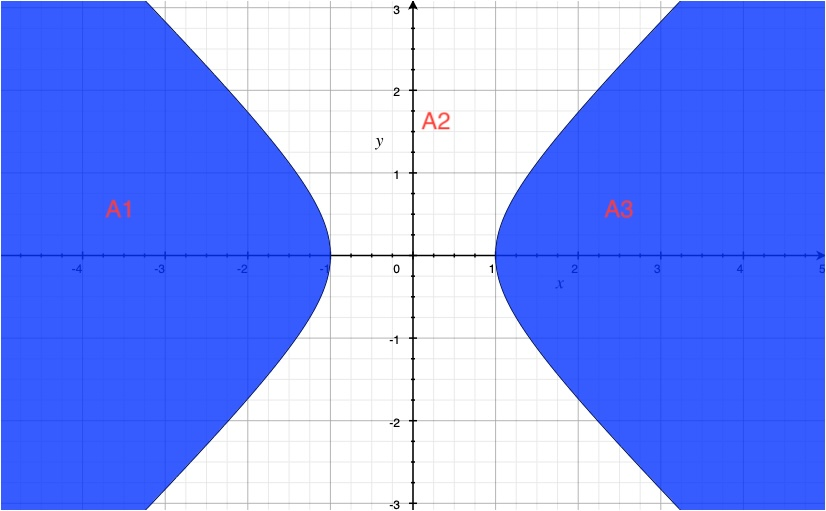
\includegraphics[width=0.65\textwidth]{Analisi2/figures/grafico_x^2-y^2-1.jpg}
        \caption{Sottografico di $2x-3y+1=0$.}\label{fig:grafico_x^2-y^2-1}
    \end{figure}
\end{example}

Dall'esempio è possibile affermare che se $f(x,y)$ è continua in $\mathbb R^2$, allora quando $f(x,y)\neq 0$ (è importante che sia diverso da 0) definisce un aperto del piano dato dall'unione di un certo numero di aperti connessi sul quale $f$ è definita ed è diversa da 0. Nell'esempio $f(x,y)\neq 0$ su $A_1\cup A_2\cup A_3$.

Supponendo gli aperti siano in un numero finito, ovvero: $A_1,\, A_2,\, \hdots, A_n$. È utile studiare il segno di $f(x,y)$ in ogni $A_i$ (quindi dove $f(x,y)\neq 0$).

\paragraph{Osservazioni sullo studio di $\boldsymbol{A_1}$ dell'esempio precedente:} In $A_1$ $f(x,y)\neq 0$, dunque $f(x,y)>0$ oppure $f(x,y)<0$. Dal momento che $f$ è continua ed il suo segno non può cambiare (per ipotesi) e $A_1$ è aperto e connesso, il segno di $f$ non cambia in $A_1$. Se così non fosse, esisterebbero in $A_1$ due punti distinti in cui $f(x,y)$ ha segno opposto e quindi, per il Teorema \ref{th:esistenza_degli_zeri} degli zeri, esisterebbe un punto $(x,y)\in A_1$ tale che $f(x,y)=0$. Quindi, $f(x,y)$ ha segno costante in $A_1$. Pertanto, per valutare il segno di $f$ in $A_1$ è sufficiente valutare il segno di $f$ in un punto qualsiasi di $A_1$ (come fatto nell'elenco dell'esempio).\\
Lo stesso ragionamento si ripete su ogni regione (piano) $A_i$ (quindi in ogni regione $A_i$ la funzione ha lo stesso segno).

\begin{example}\footnote{Slide 10-12 PDF 12.}
    Trovare il campo di esistenza $E$ delle seguenti funzioni
    \begin{equation*}
        \begin{aligned}
            f\colon E\subseteq\mathbb R^2 &\rightarrow \mathbb R.\\
            (x,y)&\mapsto z=f(x,y)
        \end{aligned}
    \end{equation*}
    \begin{enumerate}
        \item Sia $z=\sqrt{1-x^2-y^2}$, allora
        \begin{equation*}
            E=\{(x,y)\in\mathbb R^2\,|\, 1-x^2-y^2\geq 0\}=\{(x,y)\in\mathbb R^2\,|\, x^2+y^2\leq 1\}.
        \end{equation*}
        $E$ è chiuso e (quindi) limitato. Vedere Figura \ref{fig:dominio_rad_1-x^2-y^2}.
        \item Sia $z=\sqrt{1-x^2}+\sqrt{1-y^2}$, allora
        \begin{equation*}
            \begin{matrix}
                E&=&\{(x,y)\in\mathbb R^2\,|\, 1-x^2\geq 0,\, 1-y^2\geq 0\}&=&\\
                &=&\{(x,y)\in\mathbb R^2\,|\, x^2\leq 1,\, y^2\leq 1\}&=&\{(x,y)\in\mathbb R^2\,|\, -1\leq x\leq 1,\, -1\leq y\leq 1\}.
            \end{matrix}
        \end{equation*}
        $E$ è chiuso. Vedere Figura \ref{fig:dominio_rad_1-x^2+rad_1-y^2}.
        \item Sia $z=\frac{1}{\sqrt{y-\sqrt{x}}}$ funzione razionale, allora
        \begin{equation*}
            E=\{(x,y)\in\mathbb R^2\,|\, y-\sqrt{x}>0,\, x\geq 0\}=\{(x,y)\in\mathbb R^2\,|\, y>\sqrt{x},\, x\geq 0\}.
        \end{equation*}
        $E$ è un sopragrafico. Inoltre, non è aperto, non è chiuso, è illimitato. Vedere Figura \ref{fig:domino_frac_1_rad_y-radx}.
    \end{enumerate}
    \begin{figure}
    \centering
    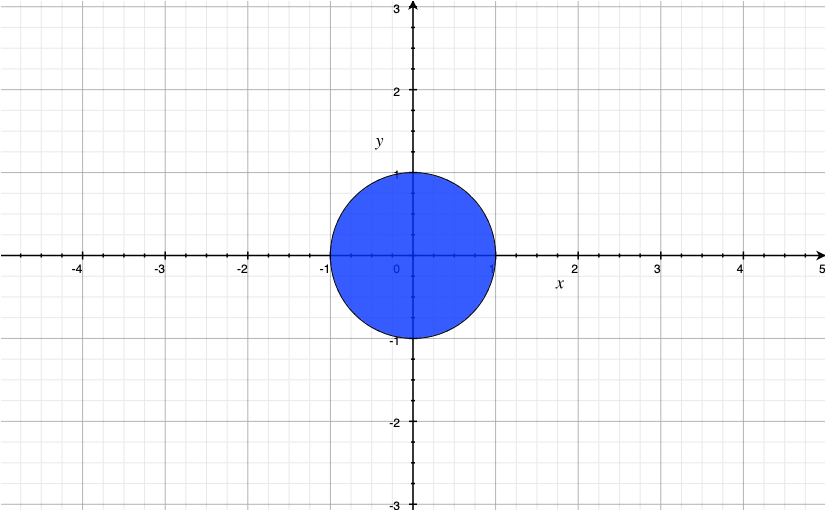
\includegraphics[width=0.65\textwidth]{Analisi2/figures/dominio_rad_1-x^2-y^2.jpg}
        \caption{Dominio $E=\{(x,y)\in\mathbb R^2\,|\, x^2+y^2\leq 1\}$ di $z=\sqrt{1-x^2-y^2}$.}\label{fig:dominio_rad_1-x^2-y^2}
    \end{figure}
    
    \begin{figure}
    \centering
    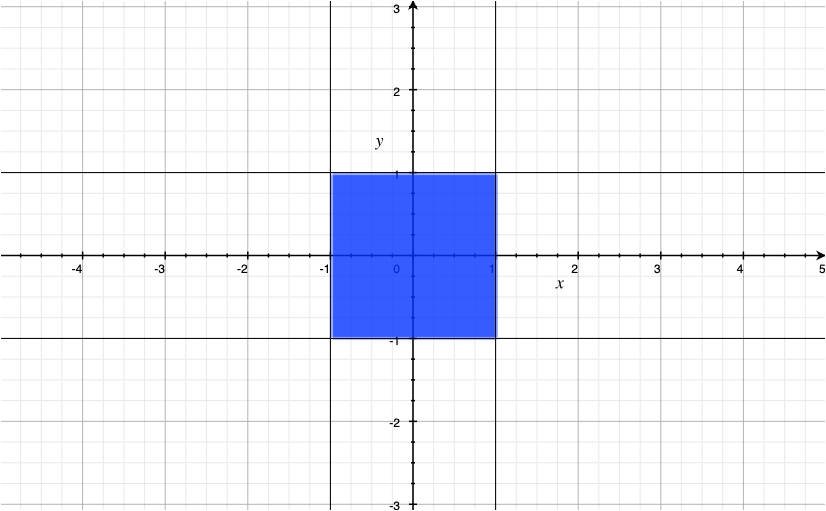
\includegraphics[width=0.65\textwidth]{Analisi2/figures/dominio_rad_1-x^2+rad_1-y^2.jpg}
        \caption{Dominio $E=\{(x,y)\in\mathbb R^2\,|\, 1-x^2\geq 0,\, 1-y^2\geq 0\}$ di $z=\sqrt{1-x^2}+\sqrt{1-y^2}$.}\label{fig:dominio_rad_1-x^2+rad_1-y^2}
    \end{figure}

    \begin{figure}
    \centering
    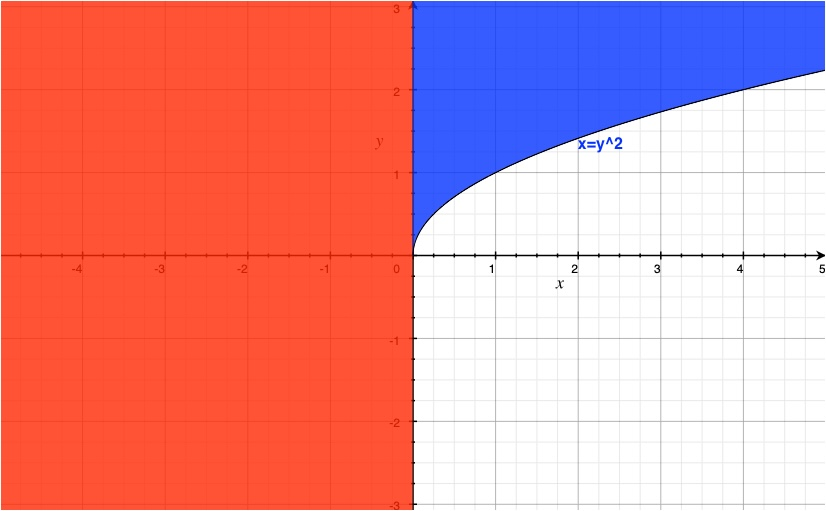
\includegraphics[width=0.65\textwidth]{Analisi2/figures/domino_frac_1_rad_y-radx.jpg}
        \caption{Dominio (in blu) $E=\{(x,y)\in\mathbb R^2\,|\, y>\sqrt{x},\, x\geq 0\}$ di $z=\frac{1}{\sqrt{y-\sqrt{x}}}$.}\label{fig:domino_frac_1_rad_y-radx}
    \end{figure}
\end{example}

\subsubsection{Esempi sulla continuità e limiti}

\begin{example}\footnote{Slide 2 PDF 13.}
	\paragraph{Testo:} Stabilire se la
	\begin{equation*}
		f(x,y)=
		\begin{cases}
			\frac{x}{\log(x^2+y^2)}&\text{ per } (x,y)\neq(0,0)\\
			0 &\text{ altrimenti}
		\end{cases}
	\end{equation*}
	funzione è continua sul suo campo di esistenza.
	\paragraph{Svolgimento:} $f:\mathbb{R}^2\rightarrow\mathbb{R}$ e affinché risulti continua deve esistere il limite della funzione, per $(x,y)\rightarrow(0,0)$ e tale limite deve valere 0, ovvero
	\begin{equation*}
		\lim_{(x,y)\rightarrow(0,0)}f(x,y)=0.
	\end{equation*}
	Valutiamo dunque
	\begin{equation*}
		\left|\frac{x}{\log(x^2+y^2)}\right|\overset{\footnotemark}{=} \left|\frac{\rho \cos\theta}{\log(\rho^2)}\right| = \frac{\rho\,|\cos\theta|}{\underbrace{2\,|\log\rho|}_{\footnotemark}}\overset{\footnotemark}{\leq} \frac{\rho}{2|\log\rho|}\underset{\rho\rightarrow0^+}{\longrightarrow}0 .
	\end{equation*}
	\addtocounter{footnote}{-2}
	\footnotetext{Passaggio in cordinate polari. Inoltre, per la relazione fondamentale dell'aritmetica $\rho^2(\cos^2\theta+\sin^2\theta) = \rho^2\cdot 1$.}
	
	\stepcounter{footnote}
	\footnotetext{Proprietà dei logaritmi.}
	
	\stepcounter{footnote}
	\footnotetext{Le funzioni trigonometriche sono comprese fra $-1$ e $1$, quindi è possibile maggiorare.}
	
	\paragraph{Nota:} È stato utilizzato il Teorema \ref{th:dei_carabinieri_2} del confronto (detto dei carabinieri) sul valore assoluto di $f(x,y)$ trasformato in coordinate polari e maggiorato da una funzione rafiale maggiore uguale a 0. Pertanto, vale quanto segue. (Non è stato considerato il caso $\rho=0$, solo quello in cui $\rho\rightarrow 0^+$.) $\qed$
	
	\noindent Dunque,
	\begin{equation*}
		\lim_{(x,y)\rightarrow(0,0)} f(x,y) = 0 = f(0,0),
	\end{equation*}
	quindi $f$ è continua in tutto $\mathbb{R}^2$.
	
\end{example}

\paragraph{Nota:} Come in Analisi 1, prolungare la continuità signidica che nel punto incriminato $f$ è posto uguale al valore al quale tende la funzione quando $(x, y)$ tendono al punto incriminato.

\begin{example}\footnote{Slide 3 PDF 13}
	\paragraph{Testo:} Stabilire se la funzione
	\begin{equation*}
		f(x,y) \overset{\footnotemark}{=} \frac{\sin(\sqrt{x^2+y^2})}{\sqrt{x^2+y^2}}\quad \forall(x,y)\in\mathbb{R}^2\backslash\{(0,0)\}
	\end{equation*}
	\footnotetext{Il quoziente sono funzioni continue in $\mathbb{R}^2$, quindi è continuo in $\mathbb{R}^2\backslash\{(0,0)\}$.}
	
	\noindent è prolungabile con continuità in $(0,0)$ e stabilire quale valore deve assumere il prolungamento di $f$ in $(0,0)$.
	\paragraph{Cosa è necessario far vedere?} È necessario definire cosa accade in $(0,0)$ e per dimostrare che il prolungamento sia continuio, che il limite di $f(x,y)$, per $(x,y)\rightarrow(0,0)$, sia il valore della funzione in tale punto.\\
	È necessario ricordare che prolungare la continuità significa che l'immagine di $f$ in $(x_0,y_0)$ deve essere uguale al limite di $f$ per $(x,y)\rightarrow(x_0,y_0)$.
	\paragraph{Svolgimento:} È possibile osservare che $\forall (x,y)\in\mathbb R^2\backslash\{(0,0)\}$, $f$ è una funzione radiale (ovvero dipende solo da $\rho$) ed è
	\begin{equation*}
		f(x,y)=f(\rho)=\frac{\sin\rho}{\rho},
	\end{equation*}
	dove $\rho = d(\rho , \underline{0})$, con $\rho=(x,y)$.\\
	Quindi,
	\begin{equation*}
		\lim_{\rho\rightarrow0^+} f(\rho)=\lim_{\rho\rightarrow 0^+} \frac{\sin\rho}{\rho}=1.
	\end{equation*}
	\paragraph{Nota:} Quindi, se la funzione prolungata in $(0,0)$ vale 1, come il limite, allora la funzione è continua nel suo dominio e nel prolungamento (che non fa parte del dominio e vale 1).$\qed$\\
	Dunque 
	\begin{equation*}
		\tilde f(x,y)=
		\begin{cases}
			\frac{\sin(\sqrt{x^2+y^2})}{\sqrt{x^2+y^2}} &\text{ se } (x,y)\neq(0,0)\\
			1 & \text{ se } (x,y)=(0,0)
		\end{cases}
	\end{equation*}
	ovvero $\tilde f$ è continua su tutto il piano.
\end{example}

\begin{example}\footnote{Slide 5 PDF 13.}
	\paragraph{Testo:} Valutare il limite
	\begin{equation*}
		\lim_{(x,y)\rightarrow(0,0)} \frac{xy(2y^2 + 2 x^3)}{x^4+y^2}.
	\end{equation*}
	\paragraph{Svolgimento:} È calcolato lungo la retta $y=mx$ (dove se $y=0$ è necessario escludere $(0,0)$):
	\begin{equation*}
		\underset{y=mx}{\lim_{(x,y)\rightarrow (0,0)}} f(x,y)=\lim_{x\rightarrow 0}f(x,mx)=\lim_{x\rightarrow 0} \frac{x\,m\,x\,(2m^2x^2+x^3)}{x^4+m^2x^2}=\lim_{x\rightarrow 0}\frac{\cancel{x^2}\,m\, [x^2(2m^2-x)]}{\cancel{x^2}(x^2+m^2)} = \lim_{x\rightarrow 0}\frac{mx^2(2m^2-x)}{x^2+m^2}=0.
	\end{equation*}
	Quindi, il limite, se esiste, è 0. È necessario mostrare che è 0. Passando in coordinate polari
	\begin{equation*}
		\begin{cases}
			x=\rho\cos\theta\\
			y=\rho\sin\theta
		\end{cases}
	\end{equation*}
	è ottenuto
	\begin{equation*}
		\begin{matrix}
			\left|\frac{\rho^2\cos\theta \sin\theta (2\rho^2\sin^2(\theta)+\rho^3\cos^3(\theta))}{\rho^4\cos^4\theta + \rho^2 \sin^2\theta}\right| &=& \left|\frac{\cancel{\rho^2}cos\theta \sin\theta (2\rho^2\sin^2(\theta)+\rho^3\cos^3(\theta))}{\cancel{\rho^2}(\rho^2\cos^4\theta + \sin^2\theta)}\right|&=& \left|\frac{2\rho^2\cos\theta\sin^3\theta + \rho^3 \cos^4\theta\sin\theta}{\rho^2 \cos^4\theta + \sin^2\theta}\right|\\\\
			&=& \left|\frac{2\rho^2\cos\theta\sin^3\theta}{\rho^2 \cos^4\theta + \sin^2\theta} + \frac{\rho^3 \cos^4\theta\sin\theta}{\rho^2 \cos^4\theta + \sin^2\theta}\right| &\overset{|x+y|\leq|x|+|y|}{\underset{\text{disug. triang.}}{\leq}}& \left|\frac{2\rho^2\cos\theta\sin^3\theta}{\rho^2 \cos^4\theta + \sin^2\theta}\right| + \left| \frac{\rho^3 \cos^4\theta\sin\theta}{\rho^2 \cos^4\theta + \sin^2\theta}\right|\\\\
			&&(\text{portate fuori cose $\geq0$})&=& \frac{2\rho^2|\cos\theta\sin^3\theta|}{\rho^2 \cos^4\theta + \sin^2\theta} + \frac{\rho^3 \cos^4\theta|\sin\theta|}{\rho^2 \cos^4\theta + \sin^2\theta}.
		\end{matrix}
	\end{equation*}
	Dunque
	\begin{equation*}
		\begin{matrix}
			|f(\rho, \theta)| &\leq& \frac{2\rho^2|\cos\theta\sin^3\theta|}{\rho^2 \cos^4\theta + \sin^2\theta} + \frac{\rho^3 \cos^4\theta|\sin\theta|}{\rho^2 \cos^4\theta + \sin^2\theta} &\overset{\footnotemark}{\leq}& \frac{2\rho^2 |\cos\theta + \sin^2\theta|}{\sin^2\theta} + \frac{\rho^3\cos^4\theta|\sin\theta|}{\rho^2 \cos^4\theta}\\\\
			&\leq& 2\rho^2 |\cos\theta\sin\theta|+\rho|\sin\theta| &=& g(\rho, \theta),
		\end{matrix}
	\end{equation*}
	
	\footnotetext{$\rho^2 \cos^4\theta + \sin^2\theta>0$ (può essere uguale a 0 ma è al denominatore). È necessario cercare di semplificare tale espressione, quindi è possibile maggiorarla con una funzione radiale (funzione dipendente solo dal raggio $\rho$) $g(\rho)$ infinitesima quando $\rho\rightarrow 0$ (cosicché anche $f$ tenda a 0).\\
	Quindi sono ricercate maggiorazioni convenienti per ogni addendo (ovvero $\frac{2\rho^2|\cos\theta\sin^3\theta|}{\rho^2 \cos^4\theta + \sin^2\theta}$ e $\frac{\rho^3 \cos^4\theta|\sin\theta|}{\rho^2 \cos^4\theta + \sin^2\theta}$). Nel precedente esempio è stata utilizzata la disuguaglianza triangolare ($|x+y|<|x|+|y|$), in questo è possibile maggiorare il denominatore considerando quanto segue:
	\begin{equation*}
		\text{Se } a,b,c \geq 0 \quad\Rightarrow\quad \frac{a}{b+c}\leq \frac{a}{b} \text{ o } \frac{a}{c}.
	\end{equation*}
	Ricercare maggiorazioni convenienti significa eliminare ciò che da fastidio per maggiorare $|f(\rho, \theta)|$ con una funzione che dopende da $\rho$. Per questo è necessario trovare una funzione radiale da moltiplicare ai due addendi $\frac{2\rho^2|\cos\theta\sin^3\theta|}{\rho^2 \cos^4\theta + \sin^2\theta}$ e $\frac{\rho^3 \cos^4\theta|\sin\theta|}{\rho^2 \cos^4\theta + \sin^2\theta}$ e che possa essere maggiorata da una costante (perché le funzioni trigonometriche sono limitate).}
	
	\noindent quindi
	\begin{equation*}
		|f(\rho, \theta)|\leq 2\rho^2\underbrace{|\cos\theta\sin\theta|}_{<\frac{1}{2}} + \rho \underbrace{|\sin\theta|}_{\leq 1}\overset{\footnotemark}{\leq} \rho^2+\rho = \rho(\rho+1) = g(\rho)\underset{\rho\rightarrow0^+}{\longrightarrow}0
	\end{equation*}
	
	\footnotetext{È necessario far vedere che esiste una funzione radiale. Per ipotesi $|\cos\theta\sin\theta|=\left|\frac{1}{2}\sin\theta\right|\leq\frac{1}{2}$ e $|\sin\theta|\leq 1$, quindi è trovata la funzione radiale infinitesima $g(\rho)=\rho^2+\rho$ che permette di applicare il teorema del confronto e che il limite sia uniforme rispetto a $\theta$.}
	\paragraph{Osservazioni:} Arrivati a $2\rho^2|\cos\theta\sin\theta|$, il processo di maggiorazione non è ancora terminato perché tale funzione è del tipo $g(\rho,\theta)$, quindi dipende anche da $\theta$. Quindi è necessario un ulteriore passo per eliminare (tramite una maggiorazione) la dipendenza da $\theta$. Inoltre, è possibile non utilizzare le coordinate polari per applicare il teorema del confronto maggiorando con una funzionen $f(x,y)$ che tende a 0 in modo uniforme rispetto alle variabili, ovvero quanto segue. $\qed$
	
	\paragraph{Svolgimento 2:} È possibile rifare l'esercizio con un metodo alternativo.
	\begin{equation*}
		\begin{matrix}
			|f(x,y)| &=& \left| \frac{xy(2y^2 + 2 x^3)}{x^4+y^2}\right| &=& \left| \frac{2xy^3 + x^4y}{x^4+y^2}\right| &=& \left|\frac{2xy^3}{x^4+y^2} + \frac{x^4y}{x^4+y^2}\right|\\\\ &\overset{|a+b|\leq|a|+|b|}{\leq}& \left|\frac{2xy^3}{x^4+y^2}\right| + \left| \frac{x^4y}{x^4+y^2}\right| &=& \frac{2|xy^3|}{x^4+y^2} + \frac{x^4|y|}{x^4+y^2} &\leq& \frac{2\cancel{y^2}|xy|}{\cancel{y^2}} +  \frac{\cancel{x^4}|y|}{\cancel{x^4}} &=&\\\\
			&&&&&=& 2|xy|+|y| &=& g(x,y) \geq 0
		\end{matrix}
	\end{equation*}
	Quindi
	\begin{equation*}
		|f(x,y)| \leq  2|xy|+|y| = g(x,y)\underset{(x,y)\rightarrow(0,0)}{\longrightarrow} 0.
	\end{equation*}
	$g$ non è una funzione radiale, è positiva e continua $\forall(x,y)\in\mathbb{R}^2$. Essere continua significa che
	\begin{equation*}
		\lim_{(x,y)\rightarrow(0,0)} g(x,y)=g(0,0)=0
	\end{equation*}
	ed è possibile applicare il teorema del confronto.
\end{example}

\begin{example}\footnote{Slide 8 PDF 13}
	\paragraph{Testo:}
	\begin{equation*}
		\lim_{(x,y)\rightarrow(0,0)} \frac{x\sin^2y+3xy^4}{x^2+2y^4}=\left[\frac{0}{0}\right]
	\end{equation*}
	\paragraph{Svolgimento:} È possibile considerare la funzione come somma di funzioni:
	\begin{equation*}
		f(x,y)=f_1(x,y)+f_2(x,y) = \frac{x\sin^2y}{x^2+2y^4} + \frac{3xy^4}{x^2+2y^4} = 
		\begin{matrix}
			x\sin^2y\rightarrow 0 \text{ come } \rho^3\\
			3xy^4\rightarrow 0 \text{ come } 3\rho^5
		\end{matrix}
	\end{equation*}
	
	\paragraph{Intermezzo:} $f_1$ ed $f_2$ hanno limite? Una delle due non ha limite. Se avessero entrambe limite allora il risultato è la somma dei due. È possibile osservare che $f_2$ sembra andare a 0 perché sopra ha una potenza superiore rispetto a sotto. $\qed$
	
	\begin{equation*}
		\lim_{(x,y)\rightarrow(0,0)} f_2(x,y) = 0,
	\end{equation*}
	infatti
	\begin{equation*}
		|f_2(x,y)|=\left|\frac{3xy^4}{x^2+2y^4}\right| = \frac{3|x|y^4}{x^2+2y^4} \leq \frac{3|x|y^4}{2y^4}=\frac{3}{2}|x|\underset{(x,y)\rightarrow(0,0)}{\longrightarrow} 0.
	\end{equation*}
	
	\paragraph{Osservazioni su $\boldsymbol{f_1}$:} L'idea è che $	\lim_{(x,y)\rightarrow(0,0)} f_1(x,y)$ non esiste perché il grado di $y^4$ è maggiore del grado di $\sin^2y$. Quindi conviene calcolare il limite lungo percorsi in cui le $x$ e $y$ pesano in modo diverso.\\
	Il numeratore e denominatore tendono a 0 rispettivamente come $\rho^3$ e come $\rho^4$. Quindi, conviene calcolare il limite lungo dei percorsi in cui $x$ e $y$ pesano in modo diverso così da mostrare comportamenti distinti, come segue. $\qed$

	\noindent \textbf{Lungo} $\boldsymbol{y=x}$ ($x$ ed $y$ pesano uguale)
	\begin{equation}\label{eq:esempio_limite_notevole}
			\underset{y=x}{\lim_{(x,y)\rightarrow(0,0)}} f_1(x,y) = \lim_{x\rightarrow 0} f_1(x,x) = \lim_{x\rightarrow 0}\frac{x\sin^2x}{x^2+2x^4} = \lim_{x\rightarrow 0}\boxed{\frac{\sin^2x}{x^2}}_{=1}\cdot\frac{x}{1+2x^2}=0
	\end{equation}
	
	\noindent \textbf{Lungo} $\boldsymbol{y=x^2}$ (così $x^2$ è paragonabile a $y^4$)
	\begin{equation*}
		\underset{y=x^2}{\lim_{(x,y)\rightarrow(0,0)}} f_1(x,y) = \lim_{y\rightarrow 0}\frac{y^2\sin^2y}{y^4+2y^4} = \lim_{y\rightarrow 0} \frac{\sin^2y}{3y^2} =\frac{1}{3} \neq 0,
	\end{equation*}
	quindi il limite di $f_1$ non esiste.\\
	Dunque
	\begin{equation*}
		\nexists \lim_{(x,y)\rightarrow(0,0)} f(x,y) = f_1 + f_2.
	\end{equation*}
	(Il limite non esiste dal momento che $f$ è la somma di $f_1$ e $f_2$ ed il limite di $f_1$ non esiste.)
\end{example}

\paragraph{Nota sui limiti:} I limiti non si fanno a pezzi, è necessario utilizzare l'algebra dei limiti: il limite di prodotti è il pordotto dei limiti quando esistono i limiti dei fattori (come in (\ref{eq:esempio_limite_notevole})). Inoltre, se è presente l'infinito, è possibile trattarlo come se fosse un numero, tranne nelle forme di indecisione ($0\cdot\infty,\, \hdots$).

\begin{example}\footnote{Slide 11 PDF 13.}
	\paragraph{Testo:}
	\begin{equation*}
		\lim_{(x,y)\rightarrow(0,0)}\left(\frac{xy^2+2y^{\frac{1}{3}}\sin^2x}{x^2+y^2}\right)e^{\left(\frac{x^2-y^2}{x^2+y^2}\right)}.
	\end{equation*}
	(Partiamo dalla prima funzione,)
	\begin{equation*}
		f_1(x,y) = \frac{xy^2+2y^{\frac{1}{3}}\sin^2x}{x^2+y^2},\quad \footnotemark
	\end{equation*}
	per la quale l'idea è che tenda a 0. \footnotetext{Pensando in coordinate polari, il denominatore va a 0 come $\rho^3$, ma il grado del nominatore è maggiore del grado del denominatore.}
	
	\noindent Passando in coordinate polari
	\begin{equation*}
		\begin{cases}
			x = \rho \cos\theta\\
			y = \rho \sin\theta
		\end{cases}
	\end{equation*}
	è verificato se è possibile maggiorare $f_1$ ed utilizzare il Teorema del confronto come segue:
	\begin{equation*}
		\begin{matrix}
				\left|\frac{\rho\cos\theta\rho^2\sin^2\theta + 2\rho^{\frac{1}{3}}(\sin\theta)^{\frac{1}{3}}\sin^2(\rho\cos\theta)}{\rho^2(\cos^2\theta+\sin^2\theta)}\right| &=& \left|\frac{\rho^{\cancel 3}\cos\theta\sin^2\theta}{\cancel{\rho^2}} + \frac{ 2\rho^{\frac{1}{3}}(\sin\theta)^{\frac{1}{3}}\sin^2(\rho\cos\theta)}{\rho^2}\right|\\\\
				&\overset{\text{disug. triang.}}{\leq}& |\rho \cos\theta\sin^2\theta| + 2 \left| \frac{ \rho^{\frac{1}{3}}(\sin\theta)^{\frac{1}{3}}\sin^2(\rho\cos\theta)}{\rho^2}\right|\\\\
				[\rho\cos\theta\leq|\rho\cos\theta|\leq\rho\rightarrow 0] &\leq& \rho |\cos\theta\sin^2\theta| + 2  \frac{ \rho^{\frac{1}{3}} |\sin\theta|^{\frac{1}{3}}|\rho\cos\theta|^2}{\rho^2}\\\\
				&=&  \rho |\cos\theta\sin^2\theta| + 2 \rho^{\frac{1}{3}} |\sin\theta|^{\frac{1}{3}}|\rho\cos\theta|^2\\\\
				&\overset{\footnotemark}{\leq}& \rho + 2\rho^{\frac{1}{3}} &=& g(\rho) \underset{\rho\rightarrow 0^+}{\longrightarrow} 0.
		\end{matrix}
	\end{equation*}
	\footnotetext{Le funzioni trigonometriche sono maggiorabili perché limitate e tramite la maggiorazione è ottenuta la funzione radiale $g$.}
	
	\noindent Data
	\begin{equation*}
		f_2(x,y) = e^{\frac{x^2-y^2}{x^2+y^2}},
	\end{equation*}
	l'esponente $\frac{x^2-y^2}{x^2+y^2}$ non ha limite per $(x,y)\rightarrow(0,0)$. Passando in coordinate polar è ottenuto
	\begin{equation*}
		\lim_{\rho\rightarrow 0^+} \frac{\cancel{\rho^2} \cos^2\theta - \rho\sin^2\theta}{\rho^2} = \lim_{\rho \rightarrow 0^+}\cos\theta-\sin\theta =\nexists.
	\end{equation*}
	È possibile dimostrare che $e^{\frac{x^2-y^2}{x^2+y^2}}$ è limitato uniformemente da una costante.
	\begin{equation*}
		\begin{matrix}
			\frac{x^2-y^2}{x^2+y^2} &\leq& \left|\frac{x^2-y^2}{x^2+y^2}\right| &=&  \frac{|x^2-y^2|}{x^2+y^2} &\leq& [|a-b| = |a+(-b)| \leq |a| + |-b|]\\
			&&&\leq& \frac{|x^2|+|-y^2|}{x^2+y^2} &=& \frac{x^2+y^2}{x^2+y^2} &=& 1
		\end{matrix}
	\end{equation*}
	Utilizzando le proprietà dell'esponenziale (in particolare che è una funzione crescente), è ottenuto che
	\begin{equation*}
		0 < e^{\frac{x^2-y^2}{x^2+y^2}} \leq e^1,
	\end{equation*}
	e dunque
	\begin{equation*}
		\left|\frac{xy^2+2y^{\frac{1}{3}}\sin^2x}{x^2+y^2}e^{\frac{x^2-y^2}{x^2+y^2}}\right| \leq e \left|\frac{xy^2+2y^{\frac{1}{3}}\sin^2x}{x^2+y^2}\right|\underset{(x,y)\rightarrow (0,0)}{\longrightarrow} 0.
	\end{equation*}
	Quindi, per il teorema del confronto, il limite di $f$ esiste ed è uguale a 0.
\end{example}

\subsection{Calcolo differenziale}\footnote{PDF 14.}
Per una funzione di una variabile $f:I\subseteq\mathbb R\rightarrow\mathbb R$ la derivata in un punto $x_0\in I$ è rappresentata da $f'(x_0)$ e definisce il tasso di variazione di $f$ nell'istante (punto) $x_0$, ovvero dal limite del rapporto incrementale (\ref{eq:limite_rapporto_incrementale}). Da $x_0$ ad $x_0+h$ c'è un solo cammino. Per le funzioni in più variabili è possibile seguire infiniti cammini, quindi è necessario chiarire cos'è una derivata in più variabili.
\subsubsection{Derivate parziali}
Il concetto di derivata di una funzione di una variabile si estende per una funzione di due variabili con la definizione di derivata parziale. Una derivata parziale rispetto ad una variabile di una funzione di $n$ variabili è, come in Analisi 1, il limite del rapporto incrementale sulla variabile interessata (mentre le altre rimangono congelate). Una funzione di $n$ variabili ha una derivata parziale per ogni variabile (quindi $f(x_1,\hdots,x_n)$ ha $n$ derivate parziali).

\begin{definition}[Derivate parziali (caso $n=2$)]\footnote{Slide 2 PDF 14.}
    Sia $f:A\subseteq\mathbb R^2\rightarrow\mathbb R$, dove $A$ aperto e $P_0=(x_0,y_0)\in A$. Le derivate parziali di $f$ rispetto alle variabili $x$ e $y$ nel punto $P_0$ sono date dai seguenti limiti purché esistano e siano finiti
    \begin{equation}\label{eq:derivata_parziale_x}
        \lim_{h\rightarrow 0}\frac{\overbrace{f(x_0+h, y_0)}^{\footnotemark}-f(x_0, y_0)}{h}:=\frac{\partial f}{\partial x}(x_0,y_0),
    \end{equation}
    \begin{equation}\label{eq:derivata_parziale_y}
        \lim_{h\rightarrow 0}\frac{f(x_0, y_0+h)-f(x_0, y_0)}{h}:=\frac{\partial f}{\partial y}(x_0,y_0).
    \end{equation}
    \footnotetext{Funzione di una variabile, $y$ è congelata.}
\end{definition}

Nel caso in cui $n>2$ è seguito lo stesso ragionamento: è fatto l'incremento sulla variabile per la quale è fatta la derivata e sono congelate le variabili non interessate (vedere Definizione \ref{def:derivata_parziale_Rn}).

Una derivata parziale è una derivata direzionale perché calcolata rispetto ad una direzione. Ad esempio: in $\mathbb R^2$ la derivata parziale rispetto ad $x$ è una derivata direzionale secondo la direzione $x$ (determinata dal versore $e_1$).

\paragraph{Perché per la derivabilità, per il gradiente e per i Teoremi è utilizzato un aperto $\boldsymbol{A}$?} Un insieme aperto ha la caratteristica topologicache ogni suo punto è interno. Nel corso sono considerati i domini, i quali sono della forma $D= A\cup\partial A$. Queste proprietà sono utili perché se una data proprietà è dimostrata per un punto dell'aperto, allora è valida nell'intorno centrato nel punto.

\paragraph{Notazione derivate parziali per $\boldsymbol{n=2}$:}
\begin{equation*}
	\begin{matrix}
		\frac{\partial f}{\partial x}(P_0)&=&f_x(x_0,y_0)&=& D_x(x_0,y_0),\\\\
		\frac{\partial f}{\partial y}(P_0) &=& f_y(x_0,y_0) &=& Dy(x_0,y_0)\\\\
		&&\text{NO } f'_x(x,y).&&
	\end{matrix}
\end{equation*}

\begin{definition}[Direzione]\footnote{Slide 2 PDF 14.}
    In $\mathbb R^n$ una direzione è un qualsiasi vettore di modulo 1.
\end{definition}
I vettori della base canonica $e_1,e_2,e_3\in\mathbb R^3$ sono le direzioni associate agli assi coordinati $x,y,z$. $e_1,e_2,e_3$ sono direzioni associate agli assi perché hanno norma uguale ad 1. Inoltre, la combinazione lineare di una direzione parallela agli assi con un qualsiasi vettore in $\mathbb R^3$ è un valore parallelo alla rispettiva asse.\\
Le direzioni sono combinate linearmente con un vettore per dare a questo una direzione nello spazio $\mathbb R^n$.

Per indicare una direzione ed un verso può essere utilizzato un versore:
\begin{definition}[Versore]
    Un versore è un vettore $\overset{\rightarrow}{v}\in\mathbb R^n$ tale che $||\overset{\rightarrow}{v}||=1$.
\end{definition}

\paragraph{N.B.:} Un versore è utilizzato per indicare una particolare direzione e verso. Inoltre, è possibile ottenere un versore da un qualsiasi vettore $v$ moltiplicandolo per il suo reciproco, ovvero: $\hat {\mathbf{v}}=\frac{\mathbf{v}}{||\mathbf {v}||}.$

Il caso delle derivate parziali di funzioni di due variabili è un caso particolare del caso generale (ovvero delle derivate direzionali, vedere Definizione \ref{def:derivate_direzionali_Rn}), dao che nel piano ci sono 2 direzioni (quelle dell'asse $x$ e dell'asse $y$). Quindi, quando si deriva in due variabili è necessario chiarire la direzione dello spostamento nel piano, ovvero: la derivata rispetto ad $x$ è quella che si muove sull'asse orizzontale. Per avere una rappresentazione grafica del concetto di derivata direzionale nelle direzioni $x$ e $y$ vedere Figura \ref{fig:rappresentazione_direzione_R2}.

\begin{figure}
    \centering
    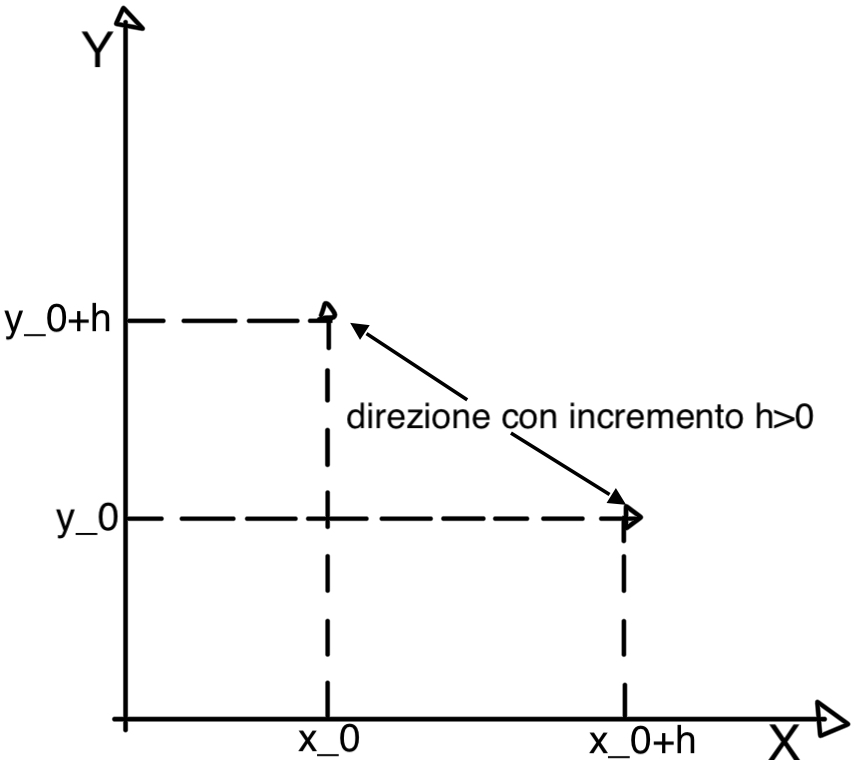
\includegraphics[width=0.65\textwidth]{Analisi2/figures/rappresentazione_direzione_R2.jpeg}
    \caption{Rappresentazione delle direzioni con incremento $h>0$.}\label{fig:rappresentazione_direzione_R2}
\end{figure}

\paragraph{N.B.:} \textbf{La Definizione \ref{def:derivata_parziale_Rn} di derivata parziale e la Definizione \ref{def:derivata_direzionale_Rn} di derivata direzionale sono equivalenti.}

\begin{definition}[Derivata parziale in $\mathbb R^n$]\label{def:derivata_parziale_Rn}\footnote{Slide 2 PDF 14.}
    Sia $f:A\subseteq\mathbb R^n\rightarrow\mathbb R$, con $A$ aperto e sia $P_0\overset{\footnotemark}{=}(x_1,x_2,\hdots, x_n)\in A$. La derivata parziale di $f$ rispetto alla variabile $x_i$ (dove $i=1,\hdots, n$) nel punto $P_0$ è data da
    \begin{equation}\label{eq:derivata_parziale_Rn}
        \lim_{h\rightarrow 0}\frac{f(x_1,\hdots,x_{i-1},x_i+h,x_{i+1},\hdots,  x_n)-f(x_1,\hdots, x_n)}{h}:=\frac{\partial f}{\partial x_i}(P_0)
    \end{equation}
    purché questo limite esista e sia finito.
\end{definition}
\footnotetext{Non è utilizzata la notazione $P_0=(x^0_1,x^0_2,\hdots, x^0_n)$ per appesantire la notazione della definizione.}

\paragraph{Quante sono le derivate parziali di una funzione di $n$ variabili?} Una funzione di $n$ variabili derivabile in un punto ha $n$ derivate parziali.

\paragraph{Notazione per le derivate parziali per $\boldsymbol{n>2}$:}
\begin{equation*}
    \frac{\partial f}{\partial x_i}(P_0)=f_{x_i}(P_0)=\frac{\partial f}{\partial x_i}(x_1,\hdots,x_n)=f_{x_i}(x_1,\hdots,x_n)=  D_{x_i}(P_0)=D_{x_i}(x_1,\hdots,x_n).
\end{equation*}

\begin{definition}[Derivabilità in $A$]\footnote{Slide 10 PDF 14.}
   Considerata $f:A\subseteq\mathbb R^n\rightarrow\mathbb R$. Se $f$ è derivabile in ogni punto $\uline x=(x_1,\hdots,x_n)\in A$, $f$ si dice derivabile in $A$ (ovvero esistono finite tutte le $n$ derivate parziali per ogni punto di $A$).
\end{definition}

In modo analogo al caso in due variabili, quando è calcolata la derivata parziale rispetto alla variabile $i$-esima, dove $i=1,\hdots,n$, sono tenute fisse tutte le variabili tranne la $i$-esima, la quale subisce un incremento. Considerando la $f$ in (\ref{eq:derivata_parziale_Rn}), sono tenute fisse tutte le variabili escluse la $i$-esima, sulla quale è applicato l'incremento. Quindi, il calcolo delle derivate parziali diventa un problema di Analisi 1 perché $f$ è come se fosse a una variabile, per il congelamento delle variabili.

Tornando alle funzioni in due variabili, le due derivate parziali sono (\ref{eq:derivata_parziale_x}) e (\ref{eq:derivata_parziale_y}), dove la funzione che subisce l'incremento in entrambi i limiti è ad una sola variabile (rispettivamente la $y$ e la $x$ sono fisse). Inoltre, quando sono state introdotte le sezioni (tracce) delle funzioni (vedere (\ref{eq:piani}) in Sezione \ref{ssec:grafico_funzione_n_variabili}) è stato spiegato che tenendo fissa una variabile è come se fosse fatta l'intersezione della funzione con il piano e quindi ottenendo il grafico di una funzione di una variabile. Quindi, quando sono date le derivate parziali (\ref{eq:derivata_parziale_x}) e (\ref{eq:derivata_parziale_y}) sono considerate le tracce della funzione lungo i piani $x=x_0$ o $y=y_0$, ovvero

\begin{equation}\label{eq:sezione_derivate_parziali}
    \begin{cases}
        z=graf\, f=f(x,y)\\
        x=x_0
    \end{cases}\rightarrow z=f(x_0,y)
    \quad\text{oppure}\quad
    \begin{cases}
        z=f(x,y)\\
        y=y_0
    \end{cases}\rightarrow z=f(x,y_0)
\end{equation}
dove $x_0$ o $y_0$ sono fissati e quindi $f$ diventa una funzione di una variabile.

Ad esempio: in (\ref{eq:derivata_parziale_x}) (ovvero $f_x(\uline x)$) è fissato $y=y_0$, quindi è come fare la traccia considerando l'intersezione della sezione con il piano $y=y_0$. Analogo fissato $x=x_0$ (ovvero con $f_y(\uline x)$).

Quindi con le sezioni del grafico ottenute tramite (\ref{eq:sezione_derivate_parziali}) sono ottenuti i grafici di curve di funzioni di una variabile nei rispettivi piani $(y,z)$ e $(x,z)$. Ciò significa che le derivate parziali delle funzioni di due variabili non sono altro che le derivate parziali, rispetto $x$ ed $y$, delle funzioni di una variabile, dove queste ultime sono le tracce della funzione in due variabili.

Infatti, se è considerata la traccia di $f(x,y)$ lungo il piano $y=y_0$ (è ottenuto)
\begin{equation*}
    f(x,y_0):=g_1(x). \footnotemark
\end{equation*}
\footnotetext{$y$ è fissa perché $y=y_0$. Quindi, come in Analisi 1, se $g_1$ è derivabile nel punto allora $g'(x)$ è la derivata parziale di $f$ rispetto ad $x$.}

Se $g_1$ è derivabile in $x_0$ significa che esiste ed è finito (il limite del rapporto incrementale di $g_1$ nel punto $x_0$, ovvero)
\begin{equation*}
    \lim_{h\rightarrow 0}\frac{g_1(x_0+h)+g_1(x_0)}{h}:=g'_1(x_0)=\frac{\partial f}{\partial x}(x_0,y_0).
\end{equation*}

Infatti
\begin{equation*}
    \lim_{h\rightarrow 0}\frac{g_1(x_0+h)+g_1(x_0)}{h}=\lim_{h\rightarrow 0}\frac{f(x_0+h,y_0)-f(x_0,y_0)}{h}.
\end{equation*}

Analogo risultato considerata la traccia di $f$ lungo il piano $x=x_0$, con
\begin{equation*}
    f(x_0,y):=g_2(y).
\end{equation*}

Se $g_2$ è derivabile in $y_0$ significa che esiste ed è finito (il limite del rapporto incrementale di $g_2$ nel punto $y_0$, ovvero)
\begin{equation*}
    \lim_{h\rightarrow 0}\frac{g_2(y_0+h)+g_2(y_0)}{h}:=g'_2(y_0)=\frac{\partial f}{\partial y}(x_0,y_0).
\end{equation*}

\paragraph{Quindi come sono calcolate le derivate?} Fissate tutte le variabili tranne l'$i$-esima è calcolato il limite del rapporto incrementale, oppure sono considerate le tracce (i due procedimenti sono simili).

\begin{example}[Calcolo di derivate parziali]\footnote{Slide 6 PDF 14.}
    Sia $f(x,y)=x\cos(x^2y^3)+x^6y^2+e^x$.
    \begin{equation}\label{eq:derivate_parziali_metodo_normale}
        \begin{matrix}
            \frac{\partial f}{\partial x}(x,y)&=& \cos(x^2y^3)-x\sin(x^2y^3)(2xy^3)+6x^5y^2+e^x&=&\cos(x^2y^3)-2x^2y^3\sin(x^2y^3)+6x^5y^2+e^x,\\\\
            \frac{\partial f}{\partial y}(P_0)&=& -x\sin(x^2y^3)(3x^2y^2)+2x^6y&=&-3x^3y^2\sin(x^2y^3)+2x^6y.
        \end{matrix}
    \end{equation}
    Calcoliamo tali derivate in $P_0=(1,2)$:
    \begin{equation*}
        \begin{matrix}
            \frac{\partial f}{\partial x}(P_0)&=& \cos(1\cdot 2^3)-2\cdot 1\cdot 2^3\sin(1\cdot 2^3)+6\cdot 1\cdot 2^2+e^1&=&\cos8 -16\sin8+24+ e,\\\\
            \frac{\partial f}{\partial y}(x,y)&=&-3\cdot 1^3\cdot 2^2\sin(1^2\,2^3)+2\cdot1^6\cdot2 &=&-12\sin8+4.
        \end{matrix}
    \end{equation*}
    \footnote{Tramite le tracce è possibile calcolare le derivate parziali nel punto $P_0$ ottenendo lo stesso risultato.}
    Utilizzando le tracce (sono fissate $x$ e $y$) $x=1$ e $y=2$, le  derivate sono calcolate come segue:\\
    (Lungo il piano $y=2$)
    \begin{equation*}
        \begin{matrix}
            f(x,2)&=&g_1(x)&\overset{\footnotemark}{=}&x\cos(8x^2)+4x^6+e^x,\\
            g'_1(x)&=&\cos(8x^2)&=&-x\sin(8x^2)16x+24x^5+e^x,\\
            g'_1(1)&=& f_x(1,2)&=& \cos(8)-16\sin8+24+e.
        \end{matrix}
    \end{equation*}
    \footnotetext{Traccia lungo il piano $y=2$. Quindi è calcolata la derivata della funzione di una variabile nel punto $x=1$ così da avere la derivata parziale rispetto ad $x$ calcolata nel punto $(1,2)$.} (Lungo il piano  $x=1$)
    \begin{equation*}
        \begin{matrix}
            f(1,y) &=& g_2(y) &=& \cos(x^2+y^2)+y^2+e\\
            g_2'(y) &=& -3y^2\sin(y^3)+2y\\
            g'_2(2) &=& -3\cdot 2^2\sin 8+ 4 &=& -12\sin 8+4.
        \end{matrix}
    \end{equation*}
    È possibile notare che le derivate parziali ottenute con i due procedimenti sono uguali.
\end{example}
\paragraph{N.B.:} Dall'esempio è possibile notare che il metodo delle tracce è più lungo del metodo utilizzando in (\ref{eq:derivate_parziali_metodo_normale}). La differenza tra i due metodi è che il (\ref{eq:derivate_parziali_metodo_normale}) presuppone che la derivata esista e se esiste è possibile calcolarla (é presupposto quindi che esista il limite del rapporto incrementale); il metodo delle tracce considera le funzioni secondo le due tracce e poi verifica che le funzioni di una variabile siano derivabili. Tuttavia, essendo $\sin,\, \cos$ e la seconda parte delle derivate funzioni regolari e appartenenti a $C^\infty$,  è naturale utilizzare il metodo (\ref{eq:derivate_parziali_metodo_normale}).

\begin{example}[Funzione derivabile ma non continua in un punto]\footnote{Slide 8 PDF 14.}
    Calcolare e esistono le derivate parziali nell'origine (ovvero in $P_0=(0,0)$) della seguente funzione:
    \begin{equation*}
        f(x,y)=
        \begin{cases}
            \frac{xy^2}{x^2+y^4} & \text{se } (x,y)\neq (0,0),\\
            0 & \text{se } (x,y)=(0,0).
        \end{cases}
    \end{equation*}
    $f:\mathbb R^2\rightarrow\mathbb R$.\\
    (Consideriamo le) tracce della funzione:
    \begin{equation*}
        \begin{matrix}
            f(x,0)=0=g_1(x),\\
            f(0,y)=0=g_2(y),
        \end{matrix}
    \end{equation*}
    e dunque (dato che $g_1$ e $g_2$ sono identicamente nulle, le derivate parziali sono)
    \begin{equation*}
        \frac{\partial f}{\partial x}(0,0)=\frac{\partial f}{\partial y}(0,0)=0.
    \end{equation*}
    Quindi $f$ è derivabile in $(0,0)$. \footnote{Dimostriamo che la funzione non è continua tramite la definizione di continuità nel punto, in particolare è mostrato (dopo la nota) che il limite di $f$ quando $(x,y)\rightarrow (0,0)$ non esiste. Per dimostrare la continuità è verificato il limite (\ref{eq:limite_continuita}) della Definizione \ref{def:continuita_funzione_n_variabili} di continuità.} Mostriamo che il limite $\lim_{(x,y)\rightarrow(0,0)}f(x,y)$ non esiste:
    \begin{equation*}
        \lim_{(x,y)\rightarrow(0,0)}\frac{xy^2}{x^2+y^4}.
    \end{equation*}
    Il candidato limite è 0 perché lungo gli assi $x=0$ e $y=0$ vale 0.\\
    Lungo l'asse $x=y^2$
    \begin{equation*}
        \underset{x=y^2}{\lim_{(x,y)\rightarrow(0,0)}}f(x,y)=\lim_{y\rightarrow 0}\frac{y^4}{y^4+y^4}=\frac{1}{2}\neq 0.
    \end{equation*}
    Dunque $f$ non è continua ma è derivabile in $(0,0)$.
\end{example}

\paragraph{N.B.:} Questo esempio aiuta a capire che se vogliamo estendere al caso in più variabili l'implicazione funzione derivabile $\rightarrow$ funzione continua, è necessario definire la differenziabilità.

\begin{definition}[Gradiente]\footnote{Slide 10 PDF 14.}
   Sia $f:A\subseteq\mathbb R^n\rightarrow\mathbb R$. Se $f$ è derivabile in $\uline x\in A$ esiste il vettore gradiente nel punto $\uline x$, il quale è definito come
   \begin{equation}
       \boldsymbol{\triangledown f(\uline x)=}\triangledown f(x_1,\hdots, x_n)=\boldsymbol{\left(\frac{\partial f}{\partial x_1}(\uline x),\hdots, \frac{\partial f}{\partial x_n}(\uline x)\right)^T}\in\mathbb R^n.
   \end{equation}
\end{definition}

\begin{example}[Gradiente in $\mathbb R^2$]\footnote{Slide 10 PDF 14.}
    Sia $f:A\subseteq\mathbb R^2\rightarrow\mathbb R$ e $P_0=(x_0,y_0)\in A$. Se $f$ è derivabile in $P_0$ allora esistono finite
    \begin{equation*}
        \frac{\partial f}{\partial x}(P_0),\; \frac{\partial f}{\partial y}(P_0),
    \end{equation*}
    quindi esiste
    \begin{equation*}
        \triangledown f(P_0)=\left(\frac{\partial f}{\partial x}(P_0),\frac{\partial f}{\partial y}(P_0)\right)=\frac{\partial f}{\partial x}(P_0)\; \uline i+ \frac{\partial f}{\partial y}(P_0)\; \uline j.
    \end{equation*}
\end{example}

\subsubsection{Significato geometrico delle derivate parziali}
\footnote{Slide 11 PDF 14.}Per dare un senso geometrico alle derivate parziali sono considerate le funzioni di 2 variabili perché è possibile disegnarne il grafico (per funzioni di $n>2$ variabili non è possibile).

\paragraph{Per le funzioni in una variabile} $f'(x_0)\in\mathbb R$ è il coefficiente angolare (la pendenza) della retta tangente al grafico di $f$ $y-t_0=f'(x_0)(x-x_0)$ per $P_0=(x_0,f(x_0))\in graf\, f\subset \mathbb R^2$.

\paragraph{Per le funzioni in due variabili} le derivate parziali sono legate rette tangenti al grafico delle curve ottenute nei piani corrispondenti fissate le tracce. Questo perché le derivate parziali sono calcolate fissate le tracce $x=x_0$ oppure $y=y_0$, come in (\ref{eq:traccia_derivata_parziale_y}) ed in (\ref{eq:traccia_derivata_parziale_x}).

(Traccia nel piano $(y,z)$)
\begin{equation}\label{eq:traccia_derivata_parziale_y}
    \begin{cases}
        x=x_0\\
        z\overset{\footnotemark}{=}f(x_0,y)
    \end{cases}
\end{equation}
\footnotetext{$f$ dipende da $y$.}

(Traccia nel piano $(x,z)$)
\begin{equation}\label{eq:traccia_derivata_parziale_x}
    \begin{cases}
        y=y_0\\
        z=f(x,y_0)
    \end{cases}
\end{equation}

\paragraph{N.B.:} Una curva è da intendersi come traiettoria (vedere la Sezione \ref{ssec:curve_Rn} nella quale sono trattate le curve).

\subsubsection{Piano tangente}\footnote{Slide 12-13 PDF 14.}
Sia $f\colon A\subseteq\mathbb R^2\rightarrow\mathbb R$, con $A$ aperto. Il grafico di $f$ $graf\,f=\{(x,y,z)\in\mathbb R^3\,|\, z=f(x,y),\, \forall (x,y)\in A\}\subset\mathbb R^3$ è un sottoinsieme dello spazio vettoriale $\mathbb R^3$ ed è una superficie in tale spazio. È una superficie perché stiamo lavorando sugli aperti e sulla regolarità della funzione.

Considerando $P_0=(x_0,y_0,z_0)\in graf\, f$, dove $z_0=f(x_0,y_0)$ vedere Figura \ref{fig:grafico_f_R3_osservazione}.

Quando sono calcolate le derivate parziali sono considerate le tracce $y=y_0$ e $x=x_0$ per avere rispettivamente le derivate parziali rispetto $x$ e $y$. Quindi, quando è considerata una traccia è intersecato il grafico di $f$ con $y=y_0$ o $x=x_0$, ovvero: taglio il grafico con $y=y_0$ per ottenere la sezione del grafico nel piano $(x,z)$, analogo per $x=x_0$.

Considerando la traccia lungo $y=y_0$ allora $T_1$ è individuata da
\begin{equation}\label{eq:traccia_g_1}
    \begin{cases}
        z=f(x,y)=f(x,y_0)=g_1(x) = f(x_0,y_0) + \frac{\partial f}{\partial x} (x_0,y_0) (x-x_0),\\
        y=y_0\quad \text{piano }(x,z)
    \end{cases}
\end{equation}

Il grafico di $g_1(x)$ è nel piano $(x,z)$ ed è rappresentato dalla curva $g_1$ in Figura \ref{fig:grafico_f_R3_osservazione}. Quanto in (\ref{eq:traccia_g_1}) può essere descritto come segue: $g_1$ è il grafico della curva $g_1(x)=f(x,y_0)=z$ nel piano $(x,z)$ passante per $P_0$ ottenuta tagliando il grafico di $f$ con $y=y_0$ ed è immaginabile come traiettoria nel piano corrispondente ottenuta dalla sezione. Ovvero: $g_1$ è l'intersezione del grafico di $f$ ($graf\, f\subset\mathbb R^3$) con il piano $(x,z)$. Inoltre, se la curva $g_1$ è derivabile, allora $g_1'(x)=\frac{\partial f}{\partial x}(x_0,y_0)$, dove $y_0=g_1=f(x,y_0)$ è il coefficiente angolare di $g_1$ in $x_0$ e il coefficiente angolare della retta $T_1$ (ovvero la retta tangente al grafico della funzione $g_1$).

Un ragionamento analogo lungo il piano $x=x_0$, traslando nel piano $(y,z)$, con
\begin{equation}\label{eq:traccia_g_2}
	\begin{cases}
		z=f(x,y)=f(x_0,y)=g_2(y) = f(x_0,y_0) + \frac{\partial f}{\partial x} (x_0,y_0) (y-y_0),\\
		x=x_0,\quad \text{piano } (y,z),
	\end{cases}
\end{equation}

dove, se $g_2(y)=f(x_0,y)$ è derivabile in $y_0$ allora $\exists g_2'(y_0)=\frac{\partial f}{\partial y}(x_0,y_0)$, con $y_0=g_2(y)=f(x_0,y)$ e questo è il coefficiente angolare di $g_2$ in $y_0$ e della retta $T_2$.

$T_1$ e $T_2$ sono rispettivamente le tangenti alle curve $g_1$ e $g_2$ (ripettivamente contenute nel piano $(x,z)$ e $(y,z)$) con rispettivi coefficienti angolari $g'_1(x_0)$ e $g_2'(x_0)$. $T_1$ e $T_2$ hanno un unico punto in comune e per esse passa un unico piano passante per il punto $P_0$. Tale piano (contente $T_1$ e $T_2$) ha equazione
 \begin{equation}\label{eq:piano_tangente_due_variabili}
 	z=f(x_0,y_0) + \frac{\partial f}{\partial x} (x_0,y_0) (x-x_0) + \frac{\partial f}{\partial x} (x_0,y_0) (y-y_0).
 \end{equation}

Il piano $z$ è passante per $P_0$, infatti in $P_0$ vale $z_0=f(x_0,y_0)$. Inoltre ogni punto $(x,y,z)$ che soddisfa (\ref{eq:traccia_g_1}) e (\ref{eq:traccia_g_2}) soddisfa anche (\ref{eq:piano_tangente_due_variabili}).
 
\paragraph{Nota:} È necessario ricordare che ci sono tante rette tangenti.

In Figura \ref{fig:grafico_f_R3_osservazione} $(x_0,y_0,0)$ è il punto sul piano $(x,y)$ di quota $z=z_0=0$ e fa parte dell'insieme di livello con $z=z_0=0$, quindi è un sottoinsieme del dominio $A$. $P_0=(x_0,y_0,z_0)$, con $z_0=f(x_0,y_0)$ è "tirato su" da $(x_0,y_0,0)$ ed è il punto $(x_0,y_0)$ di quota $z_0$.

\begin{figure}[ht]
    \centering
    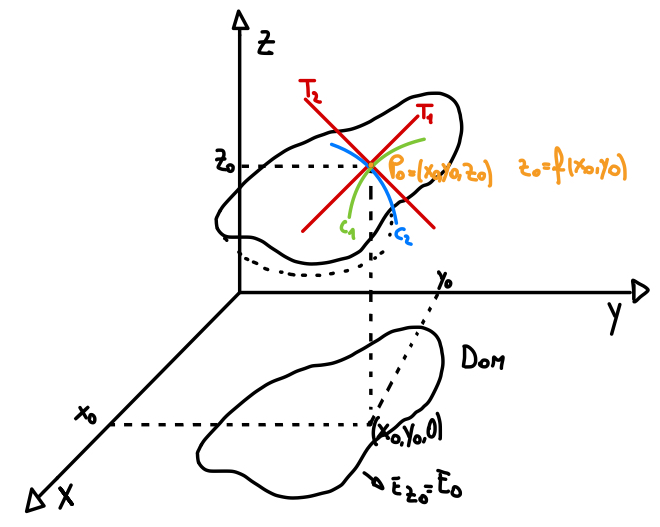
\includegraphics[width=0.65\textwidth]{Analisi2/figures/grafico_f_R3_osservazione.png}
    \caption{Grafico con rette tangenti.}\label{fig:grafico_f_R3_osservazione}
\end{figure}

\paragraph{Perché è introdotto tutto questo?} Per le funzioni di una variabile è noto che se una funzione è derivabile allora esiste ed è unica la retta tangente al grafico di $f$ passante per il punto. Inoltre, se una funzione in una variabile è derivabile allora è continua.\\
Per le funzioni in più variabili, la derivabilità non implica continuità. Quindi, per porter parlare di piano tangente, il quale fornisce una approssimazione lineare del grafico della funzione, è necessario il concetto di differenziabilità. Tutto questo perché il grafico di $f$ è in $\mathbb{R}^3$ ed è richiesta la differenziabilità per poter tracciare i piani tangente passanti per $P_0$ contenti le rette $T_1$ e $T_2$ determinate dalle sezioni.

\paragraph{Osservazioni su (\ref{eq:piano_tangente_due_variabili}):} 
\begin{enumerate}
	\item L'equazione (\ref{eq:piano_tangente_due_variabili}) si può scrivere ogni volta che $f$ è derivabile ed il piano che $f$ individua contiene le rette tangenti alle sezioni che il grafico di $f$ forma con i piani $x=x_0$ e $y=y_0$.
	\item Potrebbe venire la tentazione che l'equazione (\ref{eq:piano_tangente_due_variabili}) è l'equazione del piano tangente nella sola ipotesi che la funzione sia derivabile. In realtà è necessario che la funzione sia differenziabile affinché (\ref{eq:piano_tangente_due_variabili}) sia l'equazione del piano tangente.
	(\ref{eq:piano_tangente_due_variabili}) è la retta passante per il punto $P_0$ contenente le rette $T_1$ e $T_2$ (che altro non sono che il grafico delle sezioni della funzione).
	\item \textbf{La necessità di avere la condizione di differenziabilità è dovuta al fatto che $f$ può essere derivabile ma non continua in un punto.}
\end{enumerate}

\begin{example}[Piano tangente]\footnote{Slide 3 PDF 15.}
	Sia
	\begin{equation*}
		f(x,y)=z=x^2+y^2,
	\end{equation*}
	quindi $f:\mathbb{R}^2\rightarrow\mathbb{R}$. Le derivate di $f$ sono
	\begin{equation*}
		\frac{\partial f}{\partial x}(x,y) = 2x,\quad \frac{\partial f}{\partial y} (x,y) = 2y,
	\end{equation*}	
	quindi il gradiente è
	\begin{equation*}
		\triangledown f(x,y)=(2x,2y).
	\end{equation*}
	
	\begin{figure}[ht]
		\centering
		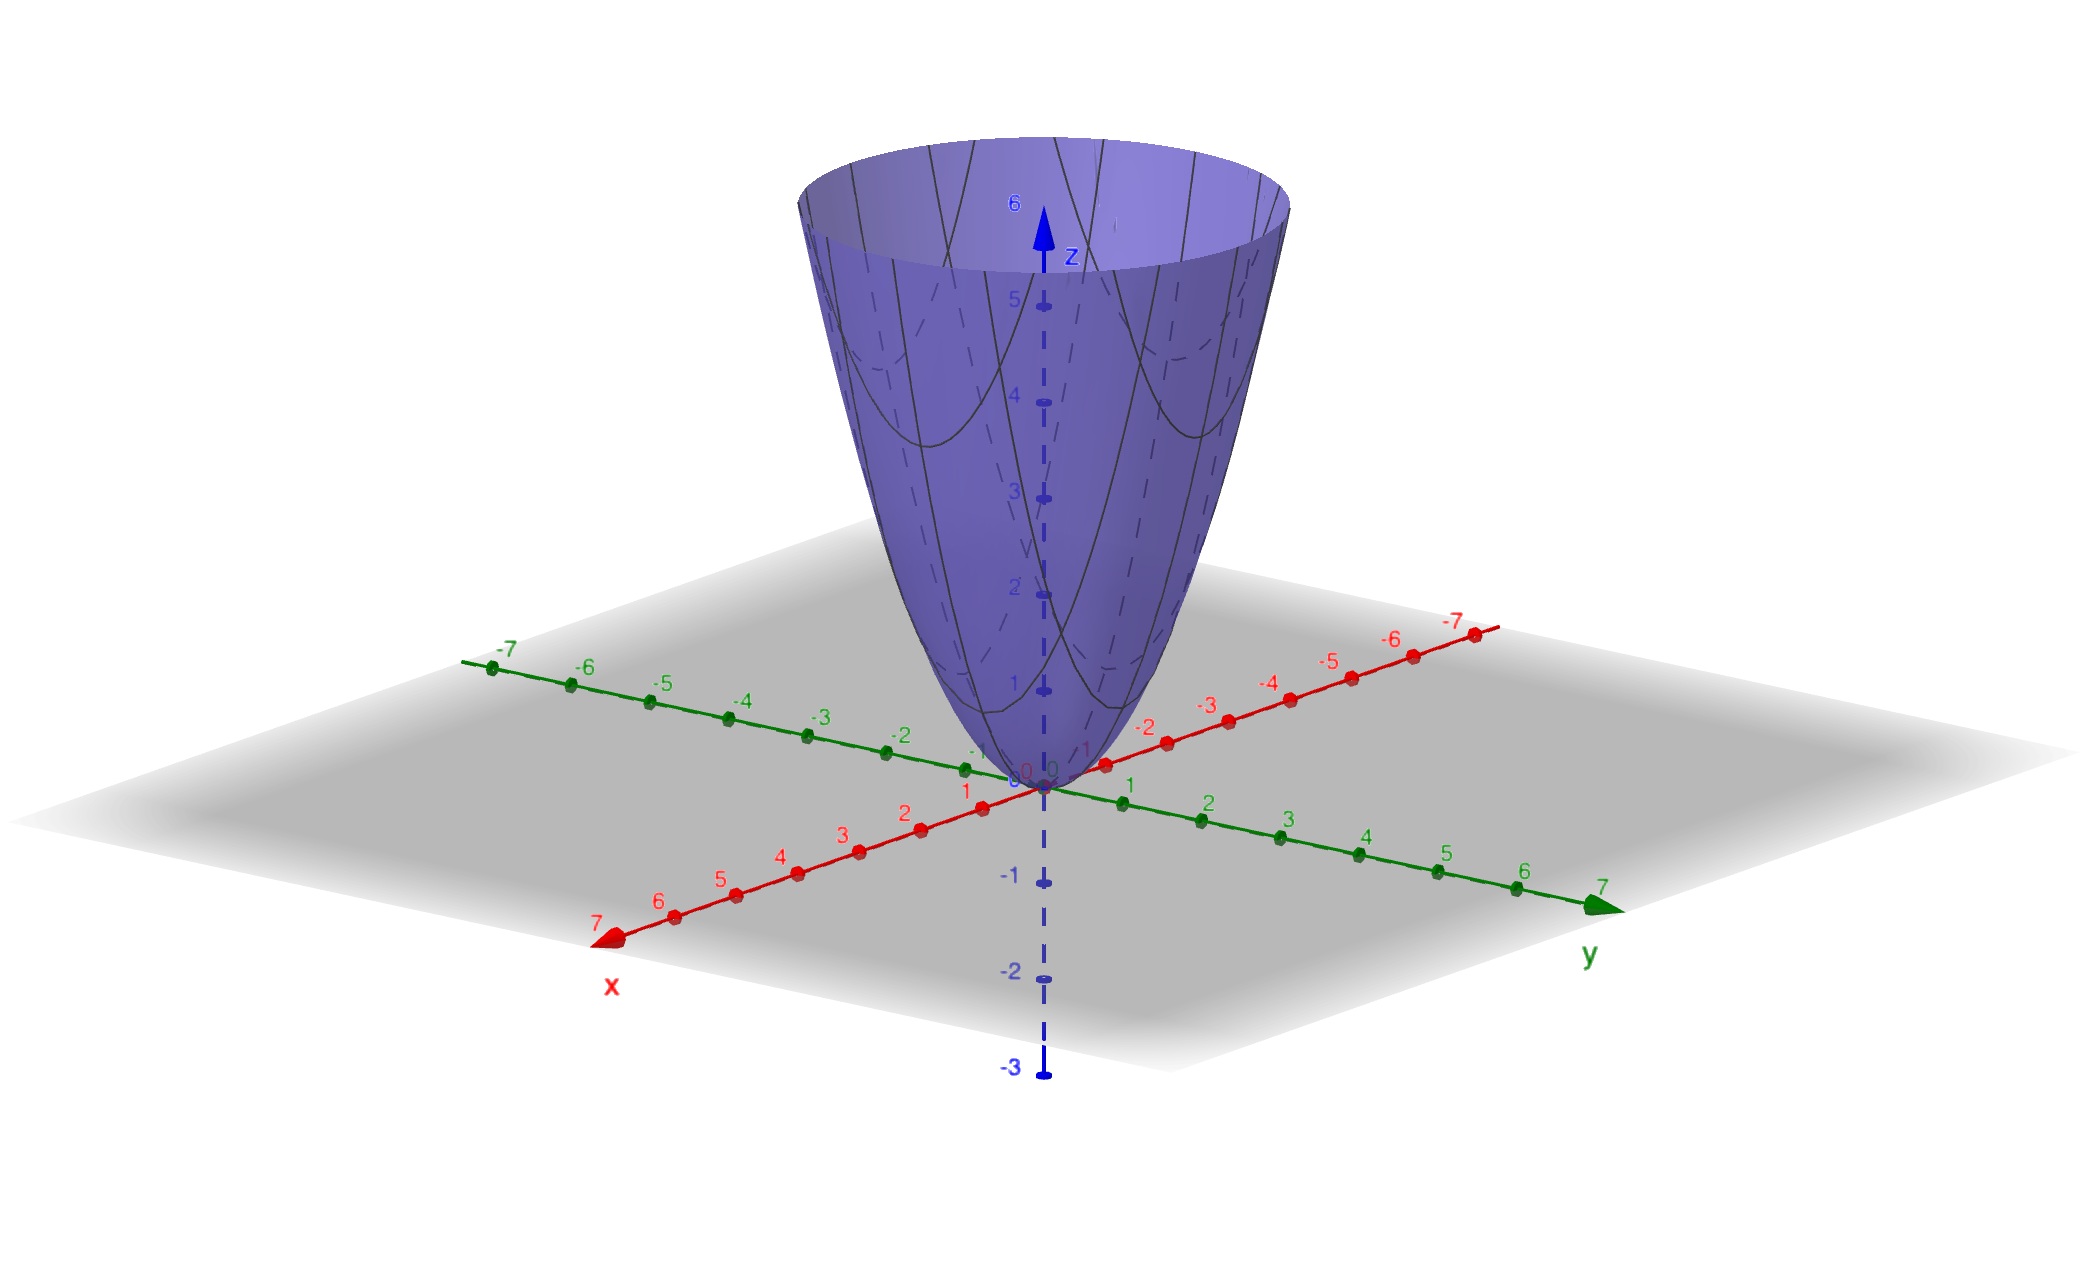
\includegraphics[width=0.65\textwidth]{Analisi2/figures/esercizio_piano_tangente.png}
		\caption{Grafico $f(x,y)=x^2+y^2$.}\label{fig:esercizio_piano_tangente}
	\end{figure}
	
	\noindent Sia $P_0=(x_0,y_0)=(0,0)$, allora
	\begin{equation*}
		\frac{\partial f}{\partial x}(P_0) = 0= \frac{\partial f}{\partial y} (P_0)
	\end{equation*}
	e quindi l'equazione del piano tangente (\ref{eq:piano_tangente_due_variabili}) passante per $P_0$ è
	\begin{equation*}
		z=f(0,0) + \frac{\partial f}{\partial x} (0,0) (x-0) + \frac{\partial f}{\partial x} (0,0) (y-0) = 0\quad (\text{ovvero il piano }(x,y)).
	\end{equation*}
	
	\paragraph{Osservazione:} Quindi, con $P_0$, il piano tangente al grafico di $f$ passante per $P_0$ è tutto $(x,y)$, ovvero il piano passante per $(0,0,0)$. Cambiando il punto (come segue) è determinato un altro piano. $\qed$
	
	\noindent Sia $P_0=(1,2)$, allora $f(1,2)=1^2+2^2=5$. Il piano tangente è
	\begin{equation*}
		z=5 + \frac{\partial f}{\partial x} (1,2) (x-1) + \frac{\partial f}{\partial x} (1,2) (y-2) = 2x + 4y - 5.
	\end{equation*}
	
\end{example}

\subsubsection{Curve in \texorpdfstring{$\boldsymbol{\mathbb R^n}$}{Rn}}\label{ssec:curve_Rn}\footnote{Slide 5 PDF 15.}
In matematica le curve sono delle applicazioni continue definite da un intervallo ad $\mathbb R^n$. In particolare, le curve piane sono delle applicazioni da un intervallo ad $\mathbb R^2$. Inoltre, il sostegno di una curva è l'immagine di una curva.
\begin{definition}[Curva in $\mathbb{R}^n$]
	\footnote{Slide 5 PDF 15.}
\end{definition}

\subsubsection{Differenziabilità}
La derivabilità di una funzione di più variabili non implica la sua continuità. Il concetto necessario da introdurre per un tipo di implicazione del genere è quello di differenziabilità (vedere Definizione (\ref{def:differenziabilita_funzione_piu_variabili})). Per le funzioni di più variabili la differenziabilità è una proprietà più forte della derivabilità perché richiede che la funzione sia derivabile e che abbia alcune proprietà legate all'approssimazione lineare ottenuta per una funzione di una variabile con l'utilizzo della derivata prima (retta tangente).

Vedere il Teorema (\ref{th:del_differenziale}) del differenziale per capire che la differenziabilità è una proprietà più forte della derivabilità.

\subsubsection{Derivate Successive}